\documentclass[10pt]{amsart}
\usepackage{A1andBox}
\usepackage{tikz-cd}
\usepackage[shortlabels]{enumitem}
\usepackage{array}
\usepackage{bbm}
\begin{document}
\title{$\A^1$-homotopy theory of log schemes}
\author{Doosung Park}
\address{Bergische Universit{\"a}t Wuppertal,
Fakult{\"a}t Mathematik und Naturwissenschaften
\\
Gau{\ss}strasse 20, 42119 Wuppertal, Germany}
\email{dpark@uni-wuppertal.de}
\subjclass[2020]{Primary 14F42; Secondary 14A21, 19E08}
\keywords{log schemes, motivic homotopy theory, localization property}
\begin{abstract}
We construct the $\A^1$-local stable motivic homotopy categories of fs log schemes.
For schemes with the trivial log structure, our construction is equivalent to the original construction of Morel-Voevodsky.
We prove the localization property.
As a consequence, we obtain the Grothendieck six functors formalism for strict morphisms of fs log schemes.
We extend $\A^1$-invariant cohomology theories of schemes to fs log schemes.
In particular, we define motivic cohomology, homotopy $K$-theory, and algebraic cobordism of fs log schemes.
For any fs log scheme log smooth over a scheme, we express cohomology of its boundary in terms of cohomology of schemes.
\end{abstract}
\maketitle


\section{Introduction}

The goal of \cite{logDM} and \cite{logSH} is to build a suitable framework of motivic homotopy theory of fs log schemes.
What makes their theory distinct from $\A^1$-homotopy theory of schemes \cite{MV} is that $\A^1$ is not inverted.
Instead, they use a new interval $\boxx:=(\P^1,\infty)$, which is the log scheme associated with the open immersion $\P^1-\{\infty\}\to \P^1$.
As a consequence, the $\infty$-category of logarithmic motives $\logDM(k)$ is constructed in \cite{logDM} for every field $k$, and the stable log motivic $\infty$-category $\logSH(S)$ is constructed in \cite{logSH} for every fs log scheme $S$.


One can incorporate various non $\A^1$-invariant cohomology theories in this setting.
For example, Hodge cohomology $H_{Zar}^p(-,\Omega^q)$ is representable in $\logDM(k)$  for every perfect field $k$ by \cite[Theorem 9.7.1]{logDM}, and topological Hochschild homology $\mathrm{THH}$ is representable in $\logSH(B)$ for every scheme $B$ by \cite{logSH}.
For the representability of Hochschild homology $\mathrm{HH}$, we refer to \cite{BLPO}.


Unfortunately, the Grothendieck six functors formalism is harder to be discovered in this non $\A^1$-invariant setting.
It seems that the localization property does not hold, which consists of the following two conditions for a strict closed immersion $i$ of fs log schemes with its open complement $j$:
\begin{itemize}
\item The induced sequence $j_\sharp j^*\to \id \to i_*i^*$ is a cofiber sequence,
\item $i_*$ is fully faithful.
\end{itemize}
If we have such a property, then $i^*$ has to be an equivalence whenever $i$ is a thickening.
However, Hodge cohomology is not nil-invariant, which is strong evidence against the localization property.
Without the localization property, the Grothendieck six functors formalism remains obscure.

The purpose of this paper is to initiate the study of Grothendieck's six functors formalism for fs log schemes after inverting $\A^1$.
Our construction of the stable motivic $\infty$-category $\SH(X)$ for fs log schemes $X$ is as follows.
We first consider the $\infty$-category of dividing Nisnevich sheaves \cite[Definition 3.1.5]{logDM} of pointed spaces on the category $\lSm/X$ of fs log schemes log smooth over $X$.
Then we apply $(\A^1\cup \ver)$-localization and $\P^1$-stabilization to construct $\SH(X)$.
The class $\ver$ consists of open immersions $j\colon U\to V$ in $\lSm/X$ such that the induced open immersion
\[
j'\colon U-\partial_X U\to V-\partial_X V
\]
is an isomorphism, where $\partial_X U$ denotes the collection of points of $U$ that are not vertical over $X$.
If $U$ is exact log smooth over $X$, then topologically, $\partial_X U$ is the relative boundary of $U$ over $X$ according to \cite[Theorem 3.7]{zbMATH05809283}.
Hence the collar neighborhood theorem ensures that inverting $j'$ is reasonable to consider at least in the case that $U$ and $V$ are exact log smooth over $X$.



What we have done in this paper are as follows:
\begin{itemize}
\item We prove that our $\SH(X)$ is equivalent to the original construction \cite[Definition 5.7]{zbMATH01194164} whenever $X$ is a scheme with the trivial log structure.
We also discuss the abelian variant $\DA(X,\Lambda)$  for any commutative ring $\Lambda$.
This is in Section 2.
\item We prove the localization property for $\SH(X)$ and $\DA(X,\Lambda)$.
As a consequence, we obtain the Grothendieck six functors formalism for strict morphisms of fs log schemes from the works of Ayoub \cite{Ayo07} and Cisinski-D\'eglise \cite{CD19}.
This consists of Section 3.
\item We provide a canonical long exact sequence of cohomology groups
\begin{align*}
\cdots
&\to
\E^{p,q}(\partial X)
\to
\E^{p,q}(X-\partial X)
\oplus
\E^{p,q}(\ul{\partial X})
\to
\E^{p,q}(\ul{X})
\\
&\to
\E^{p+1,q}(\partial X)
\to
\cdots
\end{align*}
for all base scheme $B$, object $\E\in \SH(B)$, fs log scheme $X$ log smooth over $B$, and integer $q$.
Here, $\partial X$ is the strict closed subscheme of $X$ with the reduced scheme structure consisting of the points with nontrivial log structures.
See Corollary \ref{coh.3} for the details.
\end{itemize}








Log geometry allows us to construct a refined version of the motivic tubular neighborhood. 
For example, consider the obvious immersions of fs log schemes over a field $k$ in the figure
\[
\begin{tikzpicture}
\filldraw[black!20] (0.6,0.6)--(0.6,-0.6)--(-0.6,-0.6)--(-0.6,0.6);
\filldraw[white] (0,0) circle (4pt);
\node at (0,-0.9) {$\G_m$};
\begin{scope}[shift={(3,1)}]
\filldraw[black!20]
(0.6,0.6)--(0.6,-0.6)--(-0.6,-0.6)--(-0.6,0.6);
\filldraw[ultra thick,fill=white] (0,0) circle (4pt);
\node at (0,-0.9) {$\A_\N$};
\end{scope}
\begin{scope}[shift={(3,-1)}]
\filldraw[black!20]
(0.6,0.6)--(0.6,-0.6)--(-0.6,-0.6)--(-0.6,0.6);
\node at (0,-0.9) {$\A^1$};
\end{scope}
\begin{scope}[shift={(6,1)}]
\draw[ultra thick] (0,0) circle (4pt);
\node at (0,-0.9) {$\pt_{\N}$};
\end{scope}
\begin{scope}[shift={(6,-1)}]
\filldraw (0,0) circle (2pt);
\node at (0,-0.9) {$\pt$};
\end{scope}
\draw[<-] (2.3,1)--(0.7,0.2);
\draw[<-] (2.3,-1)--(0.7,-0.2);
\draw[->] (5.6,1)--(3.7,1);
\draw[->] (5.6,-1)--(3.7,-1);
\node at (1.5,0.95) {$\widetilde{j}$};
\node at (1.5,-0.95) {$j$};
\node at (4.65,1.25) {$\widetilde{i}$};
\node at (4.65,-1.25) {$i$};
\end{tikzpicture}
\]
that also describes the Betti realizations when $k=\C$.
Levine considered the functor $i^*j_*$ in \cite{MR2302525}, which constructs the motivic punctured tubular neighborhood over $\pt$.
Dubouloz-D\'eglise-{\O}stv{\ae}r considered a similar notion, see \cite{2206.01564}.
An easy calculation shows
\[
i^*j_*\unit_{\G_m}\simeq \unit_{\pt} \oplus \Sigma^{-1,-1}\unit_{\pt},
\]
where $\unit_S$ denotes the monoidal unit in $\SH(S)$ for any fs log scheme $S$.
It is natural that $i^*j_*$ is not monoidal since this motivic tubular neighborhood is considered over the base $\pt$.
For $\cF\in \SH(\G_m)$, our refined \emph{motivic punctured tubular neighborhood of $\cF$ over $\pt_{\N}$} is defined to be $\widetilde{i}^*\widetilde{j}_*\cF$.
There is an equivalence
\[
\widetilde{i}^*\widetilde{j}_*\unit_{\G_m}\simeq \unit_{\pt_{\N}}
\]
by Proposition \ref{comp.6}.
This is an evidence that $\widetilde{i}^*\widetilde{j}_*$ is monoidal.
A systematic study of $\widetilde{i}^*\widetilde{j}_*$ requires the Grothendieck six functors formalism for fs log schemes, which we plan to establish in the forthcoming articles \cite{logGysin} and \cite{logsix}.




The $\A^1$-localization will expel various non $\A^1$-invariant cohomology theories of schemes.
Nevertheless, $\A^1$-invariant cohomology theories of schemes still remain, and our theory gives a natural way to extend such cohomology theories to fs log schemes.
In particular, we can define
\begin{itemize}
\item motivic cohomology $H_{\cM}^{p}(X,\Lambda(q))$,
\item homotopy $K$-theory $\mathrm{KH}_p(X)$,
\item and algebraic cobordism $\mathrm{MGL}^{p,q}(X)$
\end{itemize}
for all fs log scheme $X$, commutative ring $\Lambda$, and integers $p$ and $q$.

If $X$ is an fs log scheme proper and log smooth over a scheme, then our cohomology of $\partial X$ is equivalent to the cohomology of the stable homotopy type at infinity of $X-\partial X$ defined by Dubouloz-D\'eglise-{\O}stv{\ae}r, compare \cite[Remark 3.2.5]{2104.03222} and Theorem \ref{local.8}.
We also have a similar result with Wildeshaus' boundary motives, see \cite[Proposition 2.4]{zbMATH05042488}.
Hence our theory provides a logarithmic theoretical background for these notions.

This paper is a reboot of the author's thesis \cite{ParThesis} and \cite{1707.09435}.
Many classes of morphisms were inverted there for the purpose of the Grothendieck six functors formalism.
However, that makes the computation of cohomology harder.
Unlike this approach, we invert fewer morphisms that are enough to deduce the above results.



\vspace{0.1in}
\noindent \textbf{Notation and conventions.}
Every fs log scheme in this paper has a Zariski log structure.
Our standard reference for notation and terminology in log geometry is Ogus's book \cite{Ogu}.
We employ the following notation throughout the paper.

\begin{tabular}{l|l}
$\Sch$ & the category of separated noetherian schemes of finite Krull 
\\
& dimensions 
\\
$\lSch$ &  the category of separated noetherian fs log schemes  of finite
\\
& Krull dimensions
\\
$\Sm$ & the class of smooth morphisms in $\Sch$
\\
$\lSm$ & the class of log smooth morphisms in $\lSch$
\\
$\Spc$ & the $\infty$-category of spaces
\\
$\Spc_*$ & the $\infty$-category of pointed spaces
\\
$\Spt$ & the $\infty$-category of spectra
\\
$\Lambda$ & a commutative ring
\\
$\DLambda$ & the $\infty$-category of chain complexes of $\Lambda$-modules
\\
$\id\xrightarrow{ad}f_*f^*$ & the unit of an adjunction $(f^*,f_*)$
\\
$f^*f_*\xrightarrow{ad'}\id$ & the counit of an adjunction $(f^*,f_*)$
\end{tabular}


\vspace{0.1in}
\noindent \textbf{Acknowledgements.}
This research was conducted in the framework of the DFG-funded research training group GRK 2240: \emph{Algebro-Geometric Methods in Algebra, Arithmetic and Topology}.


\section{Construction of \texorpdfstring{$\SH$}{SH}}

After explaining the notation on $\infty$-categories in Subsection \ref{notation}, we review the construction of $\logSH$ in Subsection \ref{review}.
We study basic properties of vertical boundaries in Subsection \ref{vertical_boundaries}.
The notion of vertical boundaries will play an important role throughout this paper.
We also define a class of morphisms $\ver$, which we will often invert.

The purpose of Subsection \ref{removing} is to show that for $S\in \Sch$, if we invert $\A^1$ in $\logSH(S)$, then $\ver$ is inverted too.
In Subsection \ref{vertical_localizations}, we construct $\SH(S)$ for any $S\in \lSch$.
We also show that our $\SH(S)$ is equivalent to the original construction of Morel-Voevodsky if $S\in \Sch$.
The proof is done by giving an explicit description of the localization functor $L_{ver}$.
Furthermore, for $S\in \Sch$, we give an equivalence
\[
\SH(S)
\simeq
(\A^1)^{-1}\logSH(S)
\]








\subsection{Notation on \texorpdfstring{$\infty$-}{infinity }categories}
\label{notation}
\begin{df}
\label{shv.1}
Suppose $\cC$ is a presentable $\infty$-category and $\cS$ is a set of morphisms in $\cC$.
An object $X$ of $\cC$ is called \emph{$\cS$-local} if the induced map
\begin{equation}
\label{shv.1.1}
\Map_{\cC}(Y,X)\to \Map_{\cC}(Y',X)
\end{equation}
is an equivalence for every map $Y'\to Y$ in $\cS$.
A map $Y'\to Y$ is called an \emph{$\cS$-local equivalence} if \eqref{shv.1.1} is an equivalence for every $\cS$-local object $X$.

Let $\cS^{-1}\cC$ denote the full subcategory of $\cC$ consisting of $\cS$-local objects.
The inclusion functor $\cS^{-1}\cC\to \cC$ admits a left adjoint $L_{\cS}\colon \cC\to \cS^{-1}\cC$, which is called the \emph{$\cS$-localization functor}.
We refer to \cite[Section 5.5.4]{HTT} for the details.
\end{df}

\begin{const}
\label{shv.3}
Suppose $F\colon \cC\to \cC'$ is a colimit preserving functor of presentable $\infty$-categories and $\cS$ (resp.\ $\cS'$) is a set of morphisms in $\cC$ (resp.\ $\cC'$).
If $F(\cS)\subset \cS'$, then $F$ maps $\cS$-local equivalences to $\cS'$-local equivalences.
Apply \cite[Proposition 5.5.4.20]{HTT} to the composition $\cC\xrightarrow{F} \cC'\xrightarrow{L_{\cS}}\cS'^{-1}\cC'$ to obtain a canonical colimit preserving functor
\[
F\colon \cS^{-1}\cC\to \cS'^{-1}\cC'
\]
together with a commutative square
\begin{equation}
\label{shv.3.2}
\begin{tikzcd}
\cC\ar[r,"F"]\ar[d,"L_{\cS}"']&
\cC'\ar[d,"L_{\cS'}"]
\\
\cS^{-1}\cC\ar[r,"F"]&
\cS'^{-1}\cC'.
\end{tikzcd}
\end{equation}
\end{const}

\begin{df}
\label{shv.4}
For a category $\cC$ and an $\infty$-category $\cU$, we set
\[
\infPsh(\cC,\cU):=\Fun(\Nerve(\cC)^{op},\cU).
\]
This is the \emph{$\infty$-category of presheaves with values in $\cU$}.
If $\cC$ has a topology $t$, the \emph{$\infty$-category of hypercomplete $t$-sheaves with values in $\cU$} is defined to be
\[
\infShv_t(\cC,\cU):=H_t^{-1}\infPsh(\cC,\cU),
\]
where $H_t$ denotes the set of $t$-hypercovers.
\end{df}






\begin{df}
\label{shv.6}
Let $\cA$ be a class of objects of an $\infty$-category $\cC$.
We say that $\cA$ \emph{generates $\cC$} if the family of functors
\[
\Map_{\cC}(X,-)
\]
for all $X\in \cA$ is conservative.
\end{df}

\begin{lem}
\label{shv.5}
Let $F,F'\colon \cC\to \cD$ be colimit preserving functors of $\infty$-categories, and let $\cA$ be a class of objects of $\cC$ such that $\cA$ generates $\cC$.
If $\alpha\colon F\to F'$ is a natural transformation such that $\alpha(X)\colon F(X)\to F'(X)$ is an equivalence for all $X\in \cC$, then $\alpha$ is an equivalence.
\end{lem}
\begin{proof}
Let $G$ and $G'$ be right adjoints of $F$ and $F'$.
By adjunction, we only need to show that the induced map $G'(Y)\to G(Y)$ is an equivalence for all $Y\in \cD$.
Hence it suffices to show that the induced map
\[
\Map_{\cC}(X,G'(Y))\to \Map_{\cC}(X,G(Y))
\]
is an equivalence for all $X\in \cA$ and $Y\in \cD$.
By adjunction again, we finish the proof.
\end{proof}


\subsection{Review of the construction of \texorpdfstring{$\logSH$}{logSH}}
\label{review}

In this subsection, we review the construction of $\logSH$ in \cite{logSH}.
See also \cite{logDMCras}.

We begin with recalling the dividing Nisnevich topology.

\begin{df}
A morphism  in $\lSch$ is called a \emph{dividing cover} if it is a surjective proper log \'etale monomorphism.
\end{df}

Suppose $\cC$ has an initial object.
Recall from \cite[Definition 2.1]{Voe10a} that a \emph{cd-structure $P$ on $\cC$} is a collection of commutative squares
\begin{equation}
\label{top.0.1}
Q
:=
\begin{tikzcd}
Y'\ar[d]\ar[r]&
Y\ar[d]
\\
X'\ar[r]&
X
\end{tikzcd}
\end{equation}
that is closed under isomorphisms.
Such a square is called a \emph{$P$-distinguished square}.
We refer to \cite[Definitions 2.10]{Voe10a} and \cite[Definitions 3.3.22, 3.4.2]{logDM} for the definitions of regular, quasi-bounded, and squareable cd-structures.



\begin{exm}
Suppose $S\in \lSch$ and $Q$ is a commutative square in $\lSm/S$ of the form \eqref{top.0.1}.
\begin{enumerate}
\item[(i)] We say that $Q$ is a \emph{strict Nisnevich distinguished square} if every morphism in $Q$ is strict and the underlying square  $\ul{Q}$ of schemes is a Nisnevich distinguished square.
\item[(ii)] We say that $Q$ is a \emph{dividing distinguished square} if $X'=Y'=\emptyset$ and $Y\to X$ is a dividing cover.
\item[(iii)] We say that $Q$ is a \emph{dividing Nisnevich distinguished square} if $Q$ is either a strict Nisnevich or dividing distinguished square.
\end{enumerate}

The collections of such squares are called the \emph{strict Nisnevich, dividing,} and \emph{dividing Nisnevich cd-structures} respectively.
Their associated topologies are called the \emph{strict Nisnevich, dividing,} and \emph{dividing Nisnevich topologies}.

According to \cite[Proposition 3.3.30]{logDM}, the strict Nisnevich, dividing, and dividing Nisnevich cd-structures on $\lSm/S$ are quasi-bounded, regular, and squareable.
\end{exm}

\begin{df}
For every fan $\Sigma$, let $\T_\Sigma$ be the fs log scheme whose underlying scheme is the toric variety associated with $\Sigma$ and whose log structure is the compactifying log structure associated with the open immersion from the torus of the toric variety.

If $B\in \Sch$ and $P$ is an fs monoid, we set
\[
\G_{m,B}:=\G_m\times B,
\;
\A_{P,B}:=\A_P\times B,
\;
\T_{\Sigma,B}:=\T_{\Sigma}\times B.
\]
\end{df}


Next, we recall the definition of premotivic $\infty$-categories in \cite{logSH}, which is a direct generalization of premotivic triangulated categories in \cite{CD19}.



\begin{df}
\label{shv.7}
Suppose $\bC$ is a category with a class of morphisms $\cP$ that contains all isomorphisms and is closed under compositions and pullbacks.
Let
\[
\sT
\colon
\Nerve(\bC)^{op}
\to
\CAlg(\PrL)
\]
be a functor of $\infty$-categories.
For a morphism $f$ in $\bC$, we set $f^*:=\sT(f)$.
A right adjoint of $f^*$ is denoted by $f_*$.
We say that $\sT$ is a \emph{$\cP$-premotivic $\infty$-category over $\bC$} if the following conditions are satisfies:
\begin{enumerate}
\item[(i)]
For every morphism $f$ in $\cP$, $f^*$ admits a left adjoint $f_\sharp$.
\item[(ii)]
For every cartesian square
\[
\begin{tikzcd}
X'\ar[r,"g'"]\ar[d,"f'"']&
X\ar[d,"f"]
\\
S'\ar[r,"g"]&
S
\end{tikzcd}
\]
in $\bC$ such that $f\in \cP$, the Beck-Chevalley transformation
\[
Ex\colon f_\sharp' g'^* \to g^*f_\sharp
\]
is an equivalence.
\item[(iii)] For every morphism $f$ in $\cP$, the Beck-Chevalley transformation
\[
Ex\colon
f_\sharp((-)\otimes f^*(-))
\to
f_\sharp (-) \otimes (-)
\]
is an equivalence.
\end{enumerate}
For $S\in \bC$, let $\unit_S$ (or simply $\unit$) be the monoidal unit in $\sT(S)$.
If $f\colon X\to S$ is a morphism in $\cP$, then we set $M(X):=f_\sharp \unit_X$.

Let $\sT'$ be another $\cP$-premotivic $\infty$-category over $\bC$.
We say that a natural transformation $\varphi\colon \sT\to \sT'$ is a \emph{functor of $\cP$-premotivic $\infty$-categories} if the Beck-Chevalley transformation
\[
f_\sharp \varphi(Y)
\to
\varphi(X) f_\sharp
\]
is an equivalence for every $\cP$-morphism $f$.

Let $\Tri^{\otimes}$ denote the $2$-category of triangulated monoidal categories, where the $1$-morphisms are the symmetric monoidal triangulated functors, and the $2$-morphisms are the symmetric monoidal natural transformations.

The \emph{homotopy category of $\sT$}, denoted $\Ho(\sT)$, is a $2$-functor 
\[
\bC^{op}
\to
\Tri^{\otimes}
\]
obtained by taking the homotopy categories of $\sT(X)$ for all $X\in \bC$.
\end{df}


\begin{const}
\label{shv.8}
With the above notation, suppose that $\cA$ is a class of morphisms in $\sT(-)$ closed under $f^*$ for all morphisms $f$ in $\cC$, $f_\sharp$ for all morphisms $f$ in $\cP$, and $\otimes M(Y)$ for all $Y\in \cP/-$.
Then as in \cite[Section 9.1]{Robalothesis}, we can construct a $\cP$-premotivic $\infty$-category $\cA^{-1}\sT$.
Let us review the argument as follows.

Let $\cW\PrL$ the subcategory of the category $\cW\mathcal{C}\mathrm{at}_\infty$ in \cite[Construction 4.1.7.1]{HA} spanned by $(\cC,W)$ such that $\cC$ is a presentable $\infty$-category and $W$ satisfies the condition in the reference and maps $(\cC,W)\to (\cC',W')$ such that $\cC\to \cC'$ preserves colimits.
The forgetful functor
\[
for \colon \cW\PrL\to \PrL
\]
admits a fully faithful left adjoint $G$, which also admits a left adjoint $Loc^{pr}$.
We lift $\sT\colon \Nerve(\bC)\to \CAlg(\PrL)$ to form a commutative triangle
\[
\begin{tikzcd}
&
\CAlg(\mathcal{W}\PrL)\ar[d,"for"]
\\
\Nerve(\bC)\ar[r,"\sT"]\ar[ru,"\sT_{\cA}"]&
\CAlg(\PrL)
\end{tikzcd}
\]
as in \cite[Eq.\ 9.1.8]{Robalothesis}.
Compose $\sT_{\cA}$ with
\[
Loc^{pr} \colon \CAlg(\cW\PrL)\to \CAlg(\PrL)
\]
to obtain $\cA^{-1}\sT$ as in \cite[Eq.\ 9.1.10]{Robalothesis}.

The natural transformation given by the composite
\[
for \xrightarrow{ad} for\circ  G \circ Loc^{pr} \xrightarrow{\simeq} Loc^{pr}
\]
gives a functor of $\cP$-premotivic $\infty$-categories
\[
\sT \to \cA^{-1} \sT
\]
that is levelwise the $\cA$-localization.
\end{const}

\begin{df}
Let $\cC$ be a presentable symmetric monoidal $\infty$-category, and let $X$ be an object of $\cC$.
We set
\[
\Stab_X(\cC)
:=
\limit(\cdots \xrightarrow{\Omega_{X}} \cC\xrightarrow{\Omega_{X}} \cC),
\]
where $\Omega_{X}:=\ul{\Map}(-,X)$, and $\ul{\Map}$ denotes the internal mapping space.
See \cite[Section 2.2.1]{zbMATH06374152} for the details.

If the cyclic permutation $(123)$ on $X\otimes X\otimes X$ is equivalent to the identity map, then there exists a presentable symmetric monoidal $\infty$-category whose underlying $\infty$-category is $\Stab_X(\cC)$ by \cite[Corollary 2.22]{zbMATH06374152}.
\end{df}



\begin{df}
\label{logSH.1}
In $\A^1$-homotopy theory of schemes, we have the commutative diagram of $\Sm$-premotivic $\infty$-categories over $\Sch$
\[
\begin{tikzcd}
\cH \ar[r,"(-)_+"]&
\cH_* \ar[r,"\Sigma_{S^1}^\infty"]&
\SH_{S^1}\ar[r,"\Sigma_{\G_m}^\infty"]\ar[d,"{\Lambda^{(-)}}"']&
\SH\ar[d,"{\Lambda^{(-)}}"]
\\
&
&
\DAeff(-,\Lambda)\ar[r,"\Sigma_{\G_m}^\infty"]&
\DA(-,\Lambda),
\end{tikzcd}
\]
where
\begin{gather*}
\cH(S)
:=
(\A^1)^{-1}\infShv_{Nis}(\Sm/S,\Spc),
\\
\cH_*(S)
:=
(\A^1)^{-1}\infShv_{Nis}(\Sm/S,\Spc_*),
\\
\SH_{S^1}(S)
:=
(\A^1)^{-1}\infShv_{Nis}(\Sm/S,\Spt),
\\
\DAeff(S,\Lambda)
:=
(\A^1)^{-1}\infShv_{Nis}(\Sm/S,\DLambda),
\\
\SH(S)
:=
\Stab_{\G_m}(\SH_{S^1}(S)),
\;
\DA(S,\Lambda)
:=
\Stab_{\G_m}(\DAeff(S,\Lambda)).
\end{gather*}
For simplicity of notation, $\A^1$ denotes the class of projections $X\times \A^1\to X$ for $X\in \Sm/S$ (or $X\in \lSm/S$).
For a presheaf $\cF$ on $\Sm/S$ (or $\lSm/S$), let $\Lambda^{\cF}$ be the free presheaf of $\Lambda$-modules associated with $\cF$.
\end{df}

\begin{df}
Suppose $S\in \Sch$.
For $X\in \Sm/S$ with a strict normal crossing divisor $Z$ on $X$ over $S$ \cite[Definition 7.2.1]{logDM}, let $(X,Z)$ be the fs log scheme whose underlying scheme is $X$ and whose log structure is the compactifying log structure \cite[Definition III.1.6.1]{Ogu} associated with the open immersion $X-Z\to X$.
\end{df}


\begin{df}
We set $\Gmm:=(\P^1,0+\infty)$, where we regard $\P^1$ as a smooth scheme over $\Spec(\Z)$.
In \cite{logSH}, we have the commutative diagram of $\lSm$-premotivic $\infty$-categories over $\lSch$
\[
\begin{tikzcd}
\logH \ar[r,"(-)_+"]&
\logH_* \ar[r,"\Sigma_{S^1}^\infty"]&
\logSH_{S^1}\ar[r,"\Sigma_{\Gmm}^\infty"]\ar[d,"{\Lambda^{(-)}}"']&
\logSH\ar[d,"{\Lambda^{(-)}}"]
\\
&
&
\logDAeff(-,\Lambda)\ar[r,"\Sigma_{\Gmm}^\infty"]&
\logDA(-,\Lambda),
\end{tikzcd}
\]
where
\begin{gather*}
\logH(S)
:=
\boxx^{-1}\infShv_{dNis}(\lSm/S,\Spc),
\\
\logH_*(S)
:=
\boxx^{-1}\infShv_{dNis}(\lSm/S,\Spc_*),
\\
\logSH_{S^1}(S)
:=
\boxx^{-1}\infShv_{dNis}(\lSm/S,\Spt),
\\
\logDAeff(S,\Lambda)
:=
\boxx^{-1}\infShv_{dNis}(\lSm/S,\DLambda),
\\
\logSH(S)
:=
\Stab_{\Gmm}(\logSH_{S^1}(S)),
\;
\logDA(S,\Lambda)
:=
\Stab_{\Gmm}(\logDAeff(S,\Lambda)).
\end{gather*}
As before, $\boxx$ denotes the class of projections $X\times \boxx\to X$ for $X\in \lSm/S$.
There is an equivalence $\Gmm/1 \wedge S^1\simeq \P^1/1$ in $\logHpt(S)$, and hence we have an equivalence $\Sigma_{\Gmm}^\infty \Sigma_{S^1}^\infty \simeq \Sigma_{\P^1}^\infty$.

If $k$ is a field, we also have the $\infty$-category $\logDMeff(k)$, see \cite[Definition 5.2.1]{logDM}.
We set
\[
\logDM(k):=\Stab_{\Gmm}(\logDMeff(k)).
\]
For $X\in \lSm/k$, let $M(X)$ denote the associated motives in $\logDMeff(k)$ and $\logDM(k)$.
\end{df}

\subsection{Vertical boundaries}
\label{vertical_boundaries}

\begin{df}
According to \cite[Definition I.4.3.1, Remark I.4.3.2, Proposition I.4.3.3(3)]{Ogu}, a homomorphism $\theta\colon P\to Q$ of saturated monoids is called \emph{vertical} if one of the following equivalent conditions are satisfied:
\begin{enumerate}
\item[(i)] The cokernel of $\theta$ computed in the category of saturated monoids is a group.
\item[(ii)] The face of $Q$ generated by $\theta(P)$ is $Q$.
\end{enumerate}
\end{df}

\begin{prop}
\label{vert.3}
Let $\theta\colon P\to Q$ and $\eta\colon Q\to R$ be homomorphisms of saturated monoids.
\begin{enumerate}
\item[{\rm (1)}]
$\theta$ is vertical if and only if $\overline{\theta}$ is vertical.
\item[{\rm (2)}]
If $\theta$ is vertical and $G$ is a face of $Q$, then the induced homomorphism $P_{\theta^{-1}(G)}\to Q_G$ is vertical.
\item[{\rm (3)}]
If $\theta$ and $\eta$ are vertical, then $\eta\theta$ is vertical.
\item[{\rm (4)}]
If $\eta\theta$ is vertical, then $\eta$ is vertical.
\item[{\rm (5)}]
If $\eta$ is exact and $\eta\theta$ is vertical, then $\theta$ is vertical.
\end{enumerate}
\end{prop}
\begin{proof}
In \cite[Proposition I.4.3.3]{Ogu}, (1)--(4) are proven.
For (5), let $G$ be the face of $Q$ generated by $\theta(P)$.
By \cite[Proposition I.4.2.2]{Ogu}, there exists a face $H$ of $R$ such that $\eta^{-1}(H)=G$.
This implies that the face generated by $\eta\theta(P)$ is contained in $H$.
Since $\eta\theta$ is vertical, $H=R$.
Hence $G=Q$, i.e., $\theta$ is vertical.
\end{proof}

\begin{prop}
\label{vert.10}
Let
\[
\begin{tikzcd}
P\ar[d,"\theta"']\ar[r]&
P'\ar[d,"\theta'"]
\\
Q\ar[r]&
Q'
\end{tikzcd}
\]
be a cocartesian square of saturated monoids.
Then $\theta$ is vertical if and only if $\theta'$ is vertical.
\end{prop}
\begin{proof}
This follows from the fact that the cokernels of $\theta$ and $\theta'$ are isomorphic.
\end{proof}

\begin{df}
Suppose $X$ is an fs log scheme.
The \emph{boundary of $X$}, denoted $\partial X$, is the set of points of $X$ whose log structure is nontrivial.
\end{df}

\begin{df}
\label{vert.1}
Suppose $f\colon X\to S$ is a morphism of fs log schemes.
The \emph{vertical boundary of $X$ over $S$}, denoted $\partial_S X$, is the set of points $x$ of $X$ such that $\cM_{S,f(x)}\to \cM_{X,x}$ is not vertical.
We say that $f$ is \emph{vertical} if $\partial_S X=\emptyset$.
If $S=\Spec(\Z)$, then we have $\partial_{S}X = \partial X$.
\end{df}



\begin{prop}
\label{vert.7}
Let $f\colon X\to S$ be a morphism of fs log schemes.
Then $f$ is vertical if and only if $f$ admits a vertical chart $\theta\colon P\to Q$ Zariski locally on $S$ and $X$.
\end{prop}
\begin{proof}
Let $x$ be a point of $X$.
Suppose $f$ is vertical.
We can find a chart $\theta\colon P\to Q$ near $x$ and $f(x)$ such that $\ol{P}\to \ol{Q}$ is isomorphic to $\ol{\cM}_{S,f(x)}\to \ol{\cM}_{X,x}$ by \cite[Remark II.2.3.2]{Ogu}.
Use Proposition \ref{vert.3}(1) to deduce that $\theta$ is vertical.

Suppose $f$ admits a vertical chart $\theta\colon P\to Q$.
The homomorphism
$\ol{\cM}_{S,f(x)}\to \ol{\cM}_{X,x}$ is isomorphic to the induced homomorphism $P/\theta^{-1}(G)\to Q/G$ for some face $G$ of $Q$, which is vertical by Proposition \ref{vert.3}(1),(2).
\end{proof}



\begin{prop}
\label{vert.2}
Let $f\colon X\to S$ be a morphism of fs log schemes.
Then $\partial_S X$ is a closed subset of $X$.
\end{prop}
\begin{proof}
Suppose $x\in X-\partial_S X$.
Proposition \ref{vert.7} implies that there exists a neighborhood $U$ of $x$ such that the induced morphism $f\colon U\to S$ is vertical.
This shows that $X-\partial_S X$ is an open subset of $X$.
\end{proof}

As a consequence, we can regard $X-\partial_S X$ as an open subscheme of $X$.
We impose the reduced scheme structure to consider $\partial_S X$ as a strict closed subscheme of $X$.


\begin{prop}
\label{vert.9}
Let $f\colon X\to S$ and $g\colon Y\to X$ be morphisms of fs log schemes.
\begin{enumerate}
\item[{\rm (1)}]
If $f$ and $g$ are vertical, then $gf$ is vertical.
\item[{\rm (2)}]
If $gf$ is vertical, then $g$ is vertical.
\item[{\rm (3)}]
If $g$ is exact and $gf$ is vertical, then $f$ is vertical.
\item[{\rm (4)}]
If $f$ is vertical, then $Y-\partial_X Y$ is an open subscheme of $Y-\partial_S Y$.
\item[{\rm (5)}]
$Y-\partial_S Y$ is an open subscheme of $Y-\partial_X Y$.
\item[{\rm (6)}] If $g$ is exact, then $g$ maps $Y-\partial_S Y$ into $X-\partial_S X$.
\end{enumerate}
\end{prop}
\begin{proof}
Let $y$ be a point of $y$.
Apply Proposition \ref{vert.3}(3)--(5) to the induced homomorphisms
\[
\cM_{Y,y}
\to
\cM_{X,g(y)}
\to
\cM_{S,f(g(y))}
\]
to show (1)--(3).
These immediately imply (4)--(6).
\end{proof}












\begin{prop}
\label{vert.5}
Let
\[
\begin{tikzcd}
X'\ar[d,"f'"']\ar[r,"g'"]&
X\ar[d,"f"]
\\
S'\ar[r,"g"]&
S
\end{tikzcd}
\]
be a cartesian square of fs log schemes.
Then
\[
(X-\partial_S X)\times_S S'
\simeq
X'-\partial_{S'}X'.
\]
\end{prop}
\begin{proof}
Let $x'$ be a point of $X'$, and we set $x:=g'(x')$, $s':=f'(x')$, and $s:=f(x)$.
We need to show that $\cM_{S,s}\to \cM_{X,x}$ is vertical if and only if $\cM_{S',s'}\to \cM_{X',x'}$ is vertical.

The question is Zariski local on $S$, $S'$, and $X$.
Hence by \cite[Remark II.2.3.2]{Ogu}, we may assume that $f$ and $g$ admit charts $P\to Q$ and $P\to P'$ such that $\ol{P}\to \ol{Q}$ is isomorphic to $\ol{\cM}_{S,s}\to \ol{\cM}_{X,x}$ and $\ol{P}\to \ol{P'}$ is isomorphic to $\ol{\cM}_{S,s}\to \ol{\cM}_{S',s'}$.
For some face $F$ of $Q':=P'\oplus_P Q$ whose inverse images in $P'$ and $Q$ are $P'^*$ and $Q^*$, we have $\ol{\cM}_{X',x'}\simeq Q'/F$.
Use \cite[Corollaries I.2.3.8, I.4.2.16]{Ogu} to have $F=Q'^*$.
Hence $\cM_{S,s}\to \cM_{X,x}$ is vertical if and only if $P\to Q$ is vertical, and $\cM_{S's'}\to \cM_{X',x'}$ is vertical if and only if $P'\to Q'$ is vertical by Proposition \ref{vert.3}(1).
Apply Proposition \ref{vert.10} to the cocartesian square
\[
\begin{tikzcd}
P\ar[d]\ar[r]&
P'\ar[d]
\\
Q\ar[r]&
Q'
\end{tikzcd}
\]
to finish the proof.
\end{proof}



\begin{prop}
\label{vert.8}
Let $f\colon X\to S$ be a log unramified morphism of fs log schemes.
Then $f$ is vertical.
\end{prop}
\begin{proof}
Combine \cite[Proposition IV.3.4.1]{Ogu} and \cite[Lemma 5.6(1)]{zbMATH05809283}.
\end{proof}


\begin{df}
For an fs monoid $P$ such that $P^\gp$ is torsion free, let $\Spec(P)$ be the fan associated with the dual monoid of $P$ in $P^\gp$.
\end{df}



\begin{df}
\label{vert.11}
Suppose $\theta\colon \Sigma\to \Delta$ is a morphism of fans.
Let $\Sigma-\partial_{\Delta}\Sigma$ be the subfan of $\Sigma$ consisting of $\sigma\in \Sigma$ such that $\theta$ maps every nontrivial faces of $\sigma$ to a nontrivial cone of $\Delta$.
Equivalently, $\Sigma-\partial_{\Delta}\Sigma$ is the largest subfan of $\Sigma$ such that for every cone $\sigma\in \Sigma-\partial_{\Delta}\Sigma$ with $\theta(\sigma)=0$, we have $\sigma=0$.
\end{df}

\begin{prop}
Suppose $\theta\colon \Sigma\to \Delta$ is a morphism of fans.
Then there is a canonical isomorphism
\[
\T_\Sigma-\partial_{\T_\Delta}\T_\Sigma
\simeq
\T_{\Sigma-\partial_\Delta \Sigma}.
\]
\end{prop}
\begin{proof}
A homomorphism $\eta\colon P\to Q$ of fine monoids is vertical if and only if for every face $F$ of $Q$ with $\eta^{-1}(F)=P$, we have $F=Q$.
From the duality theory of cones \cite[Theorem I.2.3.12(4)]{Ogu}, we deduce the following:
$\T_\theta$ is vertical if and only if for every cone $\sigma\in \Sigma$ with $\theta(\sigma)=0$, we have $\sigma=0$.
This shows that $\T_{\Sigma-\partial_{\Delta}\Sigma}$ is the largest open subscheme of $\T_{\Sigma}$ that is vertical over $\T_\Delta$.
\end{proof}

\subsection{Removing boundaries}
\label{removing}

Throughout this subsection, we fix $B\in \Sch$ and a stable symmetric monoidal $\infty$-category $\cC$ with a functor
\[
M
\colon
\Nerve(\lSm/B) \to \cC
\]
satisfying the following properties:
\begin{itemize}
\item If $X,Y\in \lSm/B$, there exists a canonical equivalence
\[
M(X)\otimes M(Y)
\simeq
M(X\times_B Y).
\]
\item ($\A^1$-invariance) For every $X\in \lSm/B$, the map
\[
M(X\times \A^1)\to M(X)
\]
induced by the projection $X\times \A^1\to X$ is an equivalence.
\item ($\boxx$-invariance) For every $X\in \lSm/B$, the map
\[
M(X\times \boxx)\to M(X)
\]
induced by the projection $X\times \boxx\to X$ is an equivalence.
\item (Dividing Nisnevich descent) For every dividing Nisnevich distinguished triangle $Q$ in $\lSm/B$, $M(Q)$ is cocartesian.
\end{itemize}

\begin{exm}
\label{2.4}
We have the following examples of $\cC$
\begin{gather*}
(\A^1)^{-1}\logSH_{S^1}(B),
\;
(\A^1)^{-1}\logSH(B),
\;
(\A^1)^{-1}\logDAeff(B,\Lambda),
\\
(\A^1)^{-1}\logDA(B,\Lambda),
\;
(\A^1)^{-1}\logDMeff(k,\Lambda),
\;
(\A^1)^{-1}\logDM(k,\Lambda),
\end{gather*}
where $k$ is a field in the fifth and sixth ones.
\end{exm}






\begin{lem}
\label{2.2}
Suppose $r\geq 1$ is an integer and $Z_1,\ldots,Z_r$ are the axes divisors of $\A^r$.
If we set $Y:=(\A^r,Z_1+\cdots+Z_r)$ and $W:=Z_1\cap \cdots \cap Z_r$, then the induced map
\[
M(Y-W)
\to
M(Y)
\]
is an equivalence.
\end{lem}
\begin{proof}
We set $\ol{Y}:=(\P^r,Z_1+\cdots+Z_r)$, and we view $\A^r$ as the open subscheme of $\P^r$ excluding the hyperplane at $\infty$.
The square
\[
\begin{tikzcd}
Y-W\ar[d]\ar[r]&
Y\ar[d]
\\
\ol{Y}-W\ar[r]&
\ol{Y}
\end{tikzcd}
\]
is a strict Nisnevich distinguished square.
Hence we need to show that the induced map
\[
M(\ol{Y}-W)\to M(\ol{Y})
\]
is an equivalence.
Since $\ol{Y}\simeq \boxx^r$, it remains to show $M(\ol{Y}-W)\simeq M(\pt)$.

For any nonempty subset $I=\{i_1,\ldots,i_s\}\subset \{1,\ldots,r\}$, we set $Z_I:=Z_{i_1}+ \cdots + Z_{i_s}$.
Since $\ol{Y}-W=(\ol{Y}-Z_1)\cup \cdots \cup (\ol{Y}-Z_r)$, it suffices to show $M_S(\ol{Y}-Z_I)\simeq M(\pt)$ for all $I$ by dividing Nisnevich descent.
This follows from $\ol{Y}-Z_I\simeq \A^s \times \boxx^{r-s}$.
\end{proof}

\begin{prop}
\label{2.3}
For every $Y\in \lSm/B$, the induced map
\[
M(Y-\partial Y)
\to
M(Y)
\]
is an equivalence.
\end{prop}
\begin{proof}
The question is Zariski local on $Y$.
Hence we may assume that $Y$ admits a chart $P$ such that $P$ is sharp by \cite[Proposition II.2.3.7]{Ogu}.
There exists a dividing cover $Y'\to Y$ such that $\partial Y'$ is a strict normal crossing divisor by toric resolution of singularities \cite[Theorem 11.1.9]{CLStoric}.
Furthermore, the induced morphism $Y'-\partial Y'\to Y-\partial Y$ is an isomorphism.
Owing to dividing Nisnevich descent, it suffices to show that the induced map $M(Y'-\partial Y')\to M(Y')$ is an equivalence.
In other words, we reduce to the case when $\partial Y$ is a strict normal crossing divisor.

Let $Z_1,\ldots,Z_r$ be the irreducible components of $\partial Y$.
We proceed by induction on the maximum codimension $d$ of the nonempty intersections of $Z_1,\ldots,Z_r$ in $Y$.
If $d=0$, there is nothing to prove.
Hence assume $d>0$.

The question is strict Nisnevich local on $Y$.
Hence we may assume that there exists a cartesian square
\[
\begin{tikzcd}
\ul{\partial Y}\ar[d]\ar[r]&
B\times \Spec(\Z[x_1,\ldots,x_n]/(x_1\cdots x_r))\ar[d]
\\
\ul{Y}\ar[r]&
B\times \Spec(\Z[x_1,\ldots,x_n])
\end{tikzcd}
\]
such that the horizontal morphisms are \'etale and the vertical morphisms are the obvious closed immersions.

We set $W:=Z_1\cap \cdots\cap Z_r$.
In this setting, \cite[Construction 7.2.8]{logDM} gives a commutative diagram
\[
\begin{tikzcd}
W\ar[d]\ar[r,leftarrow]&
W\ar[d]\ar[r]&
W\ar[d]
\\
X\ar[r,leftarrow]&
X''\ar[r]&
X'
\end{tikzcd}
\]
such that each square is cartesian, the horizontal morphisms are \'etale, and the right vertical morphism can be identified with the obvious closed immersion
\[
W\times \Spec(\Z[v_1,\ldots,v_r]/(v_1,\ldots,v_r))
\to
W\times \Spec(\Z[v_1,\ldots,v_r]).
\]

We set $Z_i':=W\times \Spec(\Z[v_1,\ldots,v_r]/(v_i))$, $Z_i'':=Z_i\times_X X''$, $Y':=(X',Z_1'+\cdots+Z_r')$, and $Y'':=(X'',Z_1''+\cdots+Z_r'')$.
The squares
\[
\begin{tikzcd}
Y''-W\ar[r]\ar[d]&
Y''\ar[d]
\\
Y-W\ar[r]&
Y,
\end{tikzcd}
\;\;
\begin{tikzcd}
Y''-W\ar[r]\ar[d]&
Y''\ar[d]
\\
Y'-W'\ar[r]&
Y'
\end{tikzcd}
\]
are strict Nisnevich distinguished squares.
Hence the squares
\[
\begin{tikzcd}
M(Y''-W)\ar[r]\ar[d]&
M(Y'')\ar[d]
\\
M(Y-W)\ar[r]&
M(Y),
\end{tikzcd}
\;\;
\begin{tikzcd}
M(Y''-W)\ar[r]\ar[d]&
M(Y'')\ar[d]
\\
M(Y'-W')\ar[r]&
M(Y')
\end{tikzcd}
\]
are cocartesian.
By Lemma \ref{2.2}, the map $M(Y'-W)\to M(Y')$ is an equivalence.
It follows that the map $M(Y-W)\to M(Y)$ is an equivalence too.

By induction, the map $M((Y-W)-\partial (Y-W))\to M(Y-W)$ is an equivalence.
To conclude, observe that the induced morphism $(Y-W)-\partial (Y-W)\to Y-\partial Y$ is an isomorphism.
\end{proof}




\subsection{Vertical localizations}
\label{vertical_localizations}

\begin{df}
Suppose $S\in \lSch$.
Let $\ver_S$ (or $\ver$ for short) be the class of morphisms in $\lSm/S$ consisting of open immersions $U\to V$ such that $U-\partial_S U\to V-\partial_S V$ is an isomorphism.
\end{df}

\begin{prop}
\label{comp.4}
Let $f\colon S'\to S$ be a morphism in $\lSch$.
If $V\to U$ is a morphism in $\ver_S$, then the pullback $V\times_S S'\to U\times_S S'$ is a morphism in $\ver_{S'}$.
If $f$ is in $\lSm$ and $V'\to U'$ is a morphism in $\ver_{S'}$, then $V'\to U'$ is a morphism in $\ver_S$.
\end{prop}
\begin{proof}
The first claim follows from Proposition \ref{vert.5}.
For the second claim, we set $W':=V'-\partial_{S'}V'\simeq U'-\partial_{S'}U'$.
Since $W'$ is an open subscheme of $V'$, $W'-\partial_S W'$ is an open subscheme of $V'-\partial_S V'$.
On the other hand, $V'-\partial_S V'$ is an open subscheme of $W$ by Proposition \ref{vert.9}(5), so $V'-\partial_S V'$ is an open subscheme of $W-\partial_S V'$.
Hence we have $V'-\partial_S V'\simeq W'-\partial_S W'$.
We similarly have $U'-\partial_S U'\simeq W'-\partial_S W'$.
\end{proof}

Together with Construction \ref{shv.8}, we obtain an $\lSm$-premotivic $\infty$-category over $\lSch$
\[
(\A^1\cup \ver)^{-1}\infShv_{dNis}(\lSm/-,\Spc).
\]
Since $\boxx-\partial \boxx\simeq \A^1$, $\boxx$ is already inverted here.
On the other hand, $\A^1$ is already inverted in $\ver^{-1}\logH$.
Hence we have the localization functor
\begin{equation}
L_{\ver}
\colon
\logH \to (\A^1\cup \ver)^{-1}\infShv_{dNis}(\lSm/-,\Spc).
\end{equation}

\begin{rmk}
Suppose $S\in \lSch$.
Let $\ver'$ be the class of morphisms in $\lSm/S$ consisting of the open immersions $U-\partial_S U\to U$ for all $U\in \lSm/S$.
Then $\ver'$ is a subclass of $\ver$, and there is a canonical equivalence
\[
(\A^1\cup \ver')^{-1}\infShv_{dNis}(\lSm/S,\Spc)
\simeq
(\A^1\cup \ver)^{-1}\infShv_{dNis}(\lSm/S,\Spc).
\]
However, $\ver'$ does not satisfy the second claim in Proposition \ref{comp.4}.
For example, if $f\colon S'\to S$ is a morphism in $\lSm$ that is not vertical, then the identity morphism $S'\to S'$ is not in $\ver_{S}$ even though it is in $\ver_{S'}$.
\end{rmk}



\begin{const}
\label{comp.5}
Suppose $S\in \Sch$.
Let $\lambda\colon \Sm/S\to \lSm/S$ be the functor sending $X\in \Sm/S$ to $X$, and let $\omega\colon \lSm/S\to \Sm/S$ be the functor sending $Y\in \lSm/S$ to $Y-\partial Y$.
Since $\lambda$ is a left adjoint of $\omega$, we have adjoint functors
\begin{equation}
\omega^\sharp
:
\infPsh(\Sm/S,\Spc)
\rightleftarrows
\infPsh(\lSm/S,\Spc)
:
\omega_\sharp
\end{equation}
where $\omega^\sharp$ is left adjoint to $\omega_\sharp$, $\omega^\sharp (X)\simeq \lambda(X)$ for $X\in \Sm/S$, and $\omega_\sharp (X)\simeq \omega(X)$.
Since $\lambda$ and $\omega$ preserve products, $\omega^\sharp$ and $\omega_\sharp$ are monoidal.

The functor $\lambda$ maps $\A^1$ to $\A^1$ and Nisnevich distinguished squares to strict Nisnevich distinguished squares.
The functor $\omega$ maps $\A^1$ to $\A^1$ and strict Nisnevich distinguished squares to Nisnevich distinguished squares.
By Construction \ref{shv.3}, we have induced adjoint functors
\begin{equation}
\label{comp.5.1}
\omega^\sharp
:
\cH(S)
\rightleftarrows
(\A^1)^{-1}\infShv_{sNis}(\lSm/S,\Spc)
:
\omega_\sharp
\end{equation}
such that both preserve colimits.
Let $\omega^*$ be a right adjoint of $\omega_\sharp$.

For $X\in \Sm/S$, we have an equivalence $\omega_\sharp \omega^\sharp (X) \simeq X$.
Hence $\omega_\sharp \omega^\sharp \simeq \id$, so $\omega^\sharp$ and $\omega^*$ are fully faithful.

For $\cF\in (\A^1)^{-1}\infShv_{sNis}(\lSm/S,\Spc)$ and $Y\in \lSm/S$, we have an equivalence
\[
\omega^*\omega_\sharp \cF(Y)
\simeq
\cF(Y-\partial Y)=\cF(\omega(Y)).
\]
This means that $\omega^*\omega_\sharp \cF$ is $\ver$-local.
Since $\omega$ maps dividing Nisnevich distinguished squares to Nisnevich distinguished squares, $\omega^*\omega_\sharp \cF(Y)$ is $dNis$-local.
Hence
\[
\omega^*\omega_\sharp \cF(Y)\in (\A^1\cup \ver)^{-1}\infShv_{dNis}(\lSm/S,\Spc).
\]
On the other hand, if $\cF\in (\A^1\cup \ver)^{-1}\infShv_{dNis}(\lSm/S,\Spc)$, then $\omega^*\omega_\sharp \cF\simeq \cF$ since the open immersion $Y-\partial Y\to Y$ belongs to $\ver$.
It follows that the essential image of $\omega^*\omega_\sharp$ is equivalent to $(\A^1\cup \ver)^{-1}\infShv_{dNis}(\lSm/S,\Spc)$.
In summary, the localization functor
\[
L_{dNis\cup \ver}
\colon
(\A^1)^{-1}\infShv_{sNis}(\lSm/S,\Spc)
\to
(\A^1\cup \ver)^{-1}\infShv_{dNis}(\lSm/S,\Spc)
\]
satisfies
\begin{equation}
\label{comp.5.2}
L_{dNis\cup \ver}\cF(Y)
\simeq
\cF(Y-\partial Y).
\end{equation}
Furthermore, we have a canonical equivalence
\begin{equation}
\label{comp.5.3}
\cH(S)
\simeq
(\A^1\cup \ver)^{-1}\infShv_{dNis}(\lSm/S,\Spc).
\end{equation}
\end{const}




\begin{df}
\label{comp.3}
For $S\in \lSch$, we define
\begin{gather*}
\cH(S)
:=
(\A^1\cup \ver)^{-1}\infShv_{dNis}(\lSm/S,\Spc),
\\
\cH_*(S)
:=
(\A^1\cup \ver)^{-1}\infShv_{dNis}(\lSm/S,\Spc_*),
\\
\SH_{S^1}(S)
:=
(\A^1\cup \ver)^{-1}\infShv_{dNis}(\lSm/S,\Spt),
\\
\DAeff(S,\Lambda)
:=
(\A^1\cup \ver)^{-1}\infShv_{dNis}(\lSm/S,\DLambda),
\\
\SH(S)
:=
\Stab_{\G_m}(\SH_{S^1}(S)),
\;
\DA(S,\Lambda)
:=
\Stab_{\G_m}(\DAeff(S,\Lambda)).
\end{gather*}
Let $\cV$ be one of $\Spt$ and $\DLambda$.
For abbreviation, we also set
\begin{gather*}
\SH_{S^1}(S,\cV)
:=
(\A^1\cup \ver)^{-1}\infShv_{dNis}(\Sm/S,\cV),
\\
\SH(S,\cV)
:=
\Stab_{\G_m}(\SH_{S^1}(S,\cV)).
\end{gather*}
\end{df}

\begin{rmk}
When $S\in \Sch$, our definition of $\cH(S)$ is equivalent to that in \eqref{logSH.1} due to \eqref{comp.5.3}.
We can prove similar results for the other five categories, where we need to use the fact that both $\lambda$ and $\omega$ map $\G_m$ to $\G_m$ for $\SH$ and $\DA$.
We similarly have \eqref{comp.5.2} for these categories too.

Proposition \ref{comp.4} allows us to make the above categories into $\lSm$-premotivic $\infty$-categories over $\lSch$.
Furthermore, there is a commutative diagram of $\lSm$-premotivic $\infty$-categories over $\lSch$
\begin{equation}
\begin{tikzcd}[column sep=tiny, row sep=small]
\logH\ar[rr,"(-)_+"]\ar[dd,"L_{\ver}"']&&
\logH_*\ar[r,"\Sigma_{S^1}^\infty"]\ar[dd,"L_{\ver}"']&
\logSH_{S^1}\ar[rr,"\Sigma_{\Gmm}^\infty"]\ar[dd,"L_{\ver}"']\ar[rd,"\Lambda^{(-)}"']&
&
\logSH\ar[dd,"L_{\ver}",near end]\ar[rd,"\Lambda^{(-)}"]
\\
&
&
&
&
\logDAeff(-,\Lambda)\ar[rr,"\Sigma_{\Gmm}^\infty",near start,crossing over]&
&
\logDA(-,\Lambda)\ar[dd,"L_{\ver}"]
\\
\cH\ar[rr,"(-)_+"]&&
\cH_*\ar[r,"\Sigma_{S^1}^\infty"]&
\SH_{S^1}\ar[rr,"\Sigma_{\G_m}^\infty",near start]\ar[rd,"\Lambda^{(-)}"']&
&
\SH\ar[rd,"\Lambda^{(-)}"]
\\
&
&
&
&
\DAeff(-,\Lambda)\ar[rr,"\Sigma_{\G_m}^\infty"]\ar[uu,leftarrow,"L_{\ver}"',crossing over,near start]&
&
\DA(-,\Lambda).
\end{tikzcd}
\end{equation}
\end{rmk}

\begin{prop}
Suppose $B\in \Sch$ and $k$ is a field.
Then there are equivalences
\begin{gather*}
\SH_{S^1}(B)
\simeq
(\A^1)^{-1}\logSH_{S^1}(B),
\;
\SH(B)
\simeq
(\A^1)^{-1}\logSH(B),
\\
\DAeff(B,\Lambda)
\simeq
(\A^1)^{-1}\logDAeff(B,\Lambda),
\;
\DA(B,\Lambda)
\simeq
(\A^1)^{-1}\logDA(B,\Lambda),
\\
\DMeff(k,\Lambda)
\simeq
(\A^1)^{-1}\logDMeff(k,\Lambda),
\;
\DM(k,\Lambda)
\simeq
(\A^1)^{-1}\logDM(k,\Lambda).
\end{gather*}
\end{prop}
\begin{proof}
Immediate from Proposition \ref{2.3}.
\end{proof}

The equivalence $\DMeff(k,\Lambda)
\simeq
(\A^1)^{-1}\logDMeff(k,\Lambda)$ was proven in \cite[Theorem 8.2.16]{logDM} assuming resolution of singularities.


\begin{rmk}
Let $P$ be the submonoid of $\N^2$ generated by $(2,0)$, $(1,1)$, and $(0,2)$, and let $\theta \colon \N\to P$ the homomorphism sending $1$ to $(2,0)$.
Then $\A_P\to \A_{\N}$ is log smooth.
However, it is unclear whether the open immersion
\[
\A_{P}-\partial_{\A_{\N}}\A_P\to \A_P
\]
is inverted in $(\A^1)^{-1}\logSH(\A_{\N})$ or not.
Hence unlike Theorem \ref{local.5}, we do \emph{not} know how to express
\[
\map_{(\A^1)^{-1}\logSH(\A_{\N})}(M(\A_P),M(\G_m))
\]
as a mapping space in $\SH(\A^1)$.
In particular, we do \emph{not} know whether there is an equivalence
\[
(\A^1)^{-1}\logSH(\A_{\N})
\simeq
\SH(\A_{\N})
\]
or not.
This is the reason why we invert $\ver$ instead of $\boxx$ for our definition of $\SH(S)$.
\end{rmk}

\begin{prop}
\label{comp.6}
Suppose $B\in \Sch$.
Let $f\colon \A_{\N,B}\to B$ be the projection, and let $j\colon \G_{m,B} \to \A_{\N,B}$ be the obvious open immersion.
Then the natural transformation
\[
f^*\xrightarrow{ad} j_*j^* f^*
\]
is an equivalence for the $\lSm$-premotivic categories in \textup{Definition \ref{comp.3}}.
\end{prop}
\begin{proof}
Suppose $X\in \lSm/\A_{\N,B}$.
The open immersion
\[
X\times_{\A_{\N}}\G_m \to X
\]
is in $\ver_{B}$ by Proposition \ref{vert.9}(6) since $X$ is exact over $\A_{\N,B}$ by \cite[Proposition I.4.2.1(4)]{Ogu}.
Hence the morphism
\[
f_\sharp j_\sharp j^*M(X)
\to
f_\sharp M(X) 
\]
is an isomorphism.
This implies that the natural transformation $f_\sharp j_\sharp j^* \xrightarrow{ad'} f_\sharp$ is an isomorphism.
By adjunction, we get the desired natural transformation.
\end{proof}


\section{Localization property}



In this section, we prove a logarithmic analog of the localization property of Morel-Voevodsky \cite[Theorem 2.21, p.\ 114]{MV}.
See also \cite[Th\'er\`eme 4.5.36]{Ayo07} for the generalization to the setting of presheaves with values in certain model categories.

The content of Subsections \ref{preliminary} and \ref{study} is to adopt their proof in our setting.
Then we show that inverting $\A^1$ and working with the strict Nisnevich topology are enough to deduce the localization property, see Theorem \ref{loc.8}.
Based on this, we prove the localization property for our categories $\cH_*$, $\SH_{S^1}$, $\SH$, $\DAeff(-,\Lambda)$, and $\DA(-,\Lambda)$.
In Subsection \ref{consequences}, we show that the localization property implies the Grothendieck six functors formalism for strict morphisms.


\subsection{Preliminary lemmas}
\label{preliminary}
Throughout this subsection, $\cU$ is one of $\Spc$, $\Spc_*$, and $\Spt$, and $\DLambda$.

Consider the $\lSm$-premotivic $\infty$-category $\infPsh(\lSm/-,\cU)$ over $\lSch$.
Suppose $\cS$ and $\cS'$ are classes of morphisms in $\lSm$ closed under isomorphisms, compositions, and pullbacks.
If $\cS$ is contained in $\cS'$, then we have the localization functor
\[
L_{\cS'}
\colon
\cS^{-1}\infPsh(\lSm/-,\cU)
\to
\cS'^{-1}\infPsh(\lSm/-,\cU)
\]
of $\lSm$-premotivic $\infty$-categories.

\begin{df}
A \emph{henselian local fs log scheme} $X$ is an fs log scheme such that $\ul{X}$ is a henselian local scheme.
A \emph{henselization of an fs log scheme $Y$} is the fiber product $Y\times_{\ul{Y}}U$ for some henselization $U$ of $\ul{Y}$.
\end{df}


\begin{lem}
\label{loc.1}
Let $f\colon X\to S$ be a strict finite morphism in $\lSch$.
Then
\begin{equation}
\label{loc.1.2}
f_*\colon \infPsh(\lSm/X,\cU)\to \infPsh(\lSm/S,\cU)
\end{equation}
sends $sNis$-local equivalences to $sNis$-local equivalences.
\end{lem}
\begin{proof}
We argue as in \cite[Proposition 1.27, p.\ 105]{MV}.
Suppose $\cF\to \cG$ is an $sNis$-local equivalence in $\infPsh(\lSm/X,\cU)$.
For every henselization $U$ of an fs log scheme in $\lSm/S$, we need to show that the induced map
\[
f_*\cF(U)\to f_*\cG(U)
\]
is an equivalence, i.e., the map $\cF(U\times_S X)\to \cG(U\times_S X)$ is an equivalence.
This follows from the fact that $U\times_S X$ is a disjoint union of henselian local fs log schemes since $U\times_S X\to U$ is finite.
\end{proof}

Suppose $f$ is as above.
Since \eqref{loc.1.2} preserves colimits, the functor
\begin{equation}
\label{loc.1.1}
f_*\colon \infShv_{sNis}(\lSm/X,\cU)\to \infShv_{sNis}(\lSm/S,\cU)
\end{equation}
preserves colimits by Construction \ref{shv.3} and Lemma \ref{loc.1}.

For any morphism $p\colon Y\to X$ in $\lSm$, recall that we use the notation $M(Y)$ for the object $p_\sharp \unit$ in an $\lSm$-premotivic $\infty$-category.

\begin{lem}
\label{loc.2}
Suppose $f$ is as above.
Then \eqref{loc.1.1} sends $\A^1$-local equivalences to $\A^1$-local equivalences.
\end{lem}
\begin{proof}
Suppose $\cF\in \infShv_{sNis}(\lSm/X,\cU)$.
Let $p\colon \cF\otimes M(\A_X^1)\to \cF$ and $i\colon \cF\to \cF\otimes M(\A_X^1)$ be the maps induced by the structure map $\A^1\to \pt$ and the $0$-section $\pt\to \A^1$.
We need to show that 
\[
f_*(p)\colon f_*(\cF\otimes M(\A_X^1))\to f_*(\cF)
\]
is an $\A^1$-local equivalence.
Observe that $f_*$ is lax monoidal since $f^*$ is monoidal.
Consider the composition
\begin{align*}
f_*(\cF\otimes M(\A_X^1))\otimes M(\A_S^1)
&\to
f_*(\cF\otimes M(\A_X^1))\otimes f_*M(\A_X^1)
\\
&\to
f_*(\cF\otimes M(\A_X^1)\otimes M(\A_X^1))
\to
f_*(\cF\otimes M(\A_X^1)),
\end{align*}
where the first map is induced by the unit $M(\A_S^1)\to f_*f^*M(\A_S^1)\simeq f_*M(\A_X^1)$, the second map is obtained by the lax monoidality of $f_*$, and the third map is induced by the multiplication morphism $\A^1\times \A^1\to \A^1$.
Compose this with the two maps
\[
f_*(\cF\otimes M(\A_X^1))\rightrightarrows f_*(\cF\otimes M(\A_X^1))\otimes M(\A_S^1)
\]
induced by the 0-section and 1-section to obtain an $\A^1$-local equivalence $f_*(i)f_*(p)\simeq \id$.
Since we have an equivalence $f_*(p)f_*(i)\simeq \id$, we deduce that $f_*(p)$ is an $\A^1$-local equivalence.
\end{proof}

Suppose $f$ is as above.
Since \eqref{loc.1.1} preserves colimits, the functor
\begin{equation}
\label{loc.2.1}
f_*\colon (\A^1)^{-1}\infShv_{sNis}(\lSm/X,\cU)\to (\A^1)^{-1}\infShv_{sNis}(\lSm/S,\cU)
\end{equation}
preserves colimits by Construction \ref{shv.3} and Lemma \ref{loc.2}.


\begin{lem}
\label{loc.3}
Let $f\colon X\to S$ be a strict Nisnevich cover in $\lSch$.
Then
\[
f^*\colon \infPsh(\lSm/S,\cU)
\to
\infPsh(\lSm/X,\cU)
\]
detects $(sNis\cup \A^1)$-local equivalences.
\end{lem}
\begin{proof}
Suppose $\alpha\colon \cF\to \cG$ is a morphism in $\infPsh(\lSm/S,\cU)$ such that $f^*(\alpha)$ is an $(sNis\cup \A^1)$-local equivalence.
Let $\sX$ be the \v{C}ech nerve associated with $f$.
For every integer $n\geq 0$, the projection $p_n\colon \sX_n\to S$ factors through $f$.
It follows that $p_n^*(\alpha)$ is an $(sNis\cup \A^1)$-local equivalence.
Apply $p_{n\sharp}$ to obtain an $(sNis\cup \A^1)$-local equivalence
\[
\cF\otimes M(\sX_n)
\simeq
\cG\otimes M(\sX_n).
\]
Hence we obtain $(sNis\cup \A^1)$-local equivalences
\[
\cF
\simeq
\cF\otimes \colimit_{n\in \Delta}M(\sX_n)
\simeq
\cG\otimes \colimit_{n\in \Delta}M(\sX_n)
\simeq
\cG,
\]
where $\Delta$ denotes the simplex category.
\end{proof}

\begin{lem}
\label{loc.12}
Suppose
\[
\begin{tikzcd}
&Y\ar[d,"f"]
\\
Z\ar[ru,"s"]\ar[r,"i"]&
X
\end{tikzcd}
\]
is a commutative triangle of fs log schemes such that $i$ is a strict closed immersion, $f$ is log \'etale, and $\ul{X}$ is henselian.
Then there exists a unique section $X\to Y$ of $f$ extending $s$.
\end{lem}
\begin{proof}
The graph morphism $\Gamma_s\colon Z\to Z\times_X Y$ is a section of the projection $Z\times_X Y\to Z$.
Hence $\Gamma_s$ is an open immersion by \cite[Lemma A.11.2]{logDM}.
Since $i$ is a strict closed immersion, so is the projection $Z\times_X Y\to Y$.
It follows that $s$ is a strict immersion.
There exists a maximal open subscheme $U$ of $Y$ that is strict over $X$ by \cite[Lemma A.4.4]{logDM}.
Since $s$ is a strict immersion, $U$ contains the image of $s$.

If $X\to Y$ is a section of $f$, then it is an open immersion by \cite[Lemma A.11.2]{logDM} again.
Hence we need to show the claim for the commutative triangle
\[
\begin{tikzcd}
&U\ar[d]
\\
Z\ar[ru]\ar[r,"i"]&
X.
\end{tikzcd}
\]
In other words, we may assume that $f$ is strict.
In this case, $f$ is strict \'etale.
Use \cite[Th\'eor\`eme IV.18.5.11(b)]{EGA} to conclude.
\end{proof}

\begin{lem}
\label{loc.21}
Suppose $f\colon X\to S$ be a morphism of fs log schemes admitting a chart $\theta\colon P\to Q$.
Then Zariski locally on $X$, $f$ admits a chart $\eta\colon P\to R$ such that $\eta$ is injective and the cokernel of $\eta^\gp$ is torsion free.
\end{lem}
\begin{proof}
Let $\beta\colon Q\to \Gamma(X,\cM_X)$ be the given chart, and let $x$ be a point of $X$.
By \cite[Proposition II.2.3.7]{Ogu}, we may assume that there exists a chart $\beta'\colon Q'\to \Gamma(X,\cM_X)$ neat at $x$.
Note that $Q'$ is sharp.
Owing to \cite[Proposition II.2.3.9]{Ogu}, there exists homomorphisms $\kappa \colon Q\to Q'$ and $\gamma \colon Q \to \Gamma(X,\cM_X^*)$ such that $\beta=\beta'\circ \kappa+\gamma$.

Now let $\eta\colon P\to P^\gp \oplus Q'$ be the homomorphism given by $p\mapsto (p,\kappa(\theta(p)))$, and let $\delta\colon P^\gp \oplus Q'\to \Gamma(X,\cM_X)$ be the chart given by $(p,q)\mapsto \gamma^\gp( \theta^\gp(p)) + \beta'(q)$.
Then we have
\[
\delta(\eta(p))
=
\gamma(\theta(p)) + \beta'(\kappa(\theta(p)))
=
\beta(\theta(p))
\]
for $p\in P$, which implies that $\delta$ is a chart.
Since $Q'$ is sharp and saturated, $Q'^\gp$ is torsion free.
It follows that the cokernel of $\eta^\gp$ is torsion free.
\end{proof}

\begin{lem}
\label{loc.14}
Suppose $i\colon Z\to S$ is a strict closed immersion and $V\in \lSm/Z$.
Zariski locally on $V$, there exists $X\in \lSm/S$ such that $X\times_S Z\simeq V$.
\end{lem}
\begin{proof}
The question is Zariski local on $S$ and $V$, so we may assume that $V\to S$ admits a chart $\theta \colon P\to Q$ such that $\theta$ is injective and the cokernel of $\theta^\gp$ is torsion free by Lemma \ref{loc.21}.
We may also assume that $\Spec(R):=Z$, $\Spec(R'):=S$, and $V$ are affine.

Let $v$ be a point of $V$.
There exists a strict closed immersion $V\to W:=Z\times_{\A_P} \A_Q \times \A^n$ over $Z$ for some integer $n\geq 0$.
Observe that $W$ is log smooth over $Z$ by \cite[Theorem IV.3.1.8]{Ogu}.
We set $\Spec(A):=W$, and let $I$ be the ideal of $A$ such that $V\simeq \Spec(A/I)$.
By \cite[Theorem IV.3.2.2]{Ogu}, the homomorphism
\begin{equation}
\label{loc.14.1}
d\colon I/I^2 \otimes k(v)\to \Omega_{A/R}^1\otimes k(v)
\end{equation}
is injective and admits a retraction.
Use Nakayama's lemma to choose generators $a_1,\ldots,a_n$ of $I$ such that $da_1,\ldots,da_n$ are linearly independent in $\Omega_{A/R}^1\otimes k(v)$.

We set $\Spec(A'):=Y:=S\times_{\A_P}\A_Q \times \A^n$.
Choose any lifts $a_1',\ldots,a_n'$ of $a_1,\ldots,a_n$ to $A'$, and let $I'$ be the ideal of $A'$ generated by $a_1',\ldots,a_n'$.
We also set $X:=\Spec(A'/I')$.
The homomorphism
\[
d\colon I'/I'^2\otimes k(v)
\to
\Omega_{A'/R'}^1\otimes k(v)
\]
is isomorphic to \eqref{loc.14.1}, which is injective and admits a retraction.
Hence the homomorphism $d\colon I'/ I'^2\to \Omega_{A'/R'}^1$ is injective and admits a retraction on an open neighborhood $U$ of $v$ in $Y$.
By \cite[Theorem IV.3.1.8]{Ogu}, $Y$ is log smooth over $S$.
Together with \cite[Theorem IV.3.2.2]{Ogu}, we deduce that $U\times_Y X$ is log smooth over $S$.
\end{proof}

\begin{lem}
\label{loc.15}
Suppose $\cF\in \Psh(\lSm/S)$.
Then there exists a simplicial presheaf $\sX$ and a projective trivial fibration $\sX\to \cF$ such that $\sX_n$ is a coproduct of representable presheaves for all integer $n\geq 0$.
\end{lem}
\begin{proof}
A special case of \cite[Lemma 1.16, p.\ 52]{MV}.
\end{proof}

Recall that colimits commute with pullbacks in the category of sheaves by \cite[Proposition II.4.3(1)]{SGA4}.

\begin{lem}
\label{loc.13}
Suppose $S\in \lSch$ and $p\colon X\to S$ is a morphism in $\lSm$.
Consider the functor
\begin{equation}
\label{loc.13.1}
p_\sharp \colon \infPsh(\lSm/X,\Spc)\to \infPsh(\lSm/S,\Spc).
\end{equation}
For every morphism $\cF\to X$ in $\Psh(\lSm/S)$, there is a canonical equivalence
\[
p_\sharp (p^*\cF\times_{p^* X}X)\simeq \cF
\]
in $\infPsh(\lSm/S,\Spc)$, where $p^*\cF\times_{p^*X } X$ is the fiber product in $\Psh(\lSm/X)$, and the morphism $X\to p^*X$ is a right adjoint of $p_\sharp X\xrightarrow{\simeq} X$.
\end{lem}
\begin{proof}
Consider the morphism $\sX\to \cF$ in Lemma \ref{loc.15}.
Since $\sX\simeq \colimit_{n\in \Delta}\sX_n$, we reduce to the case when $\cF$ is a coproduct of representable presheaves.
We further reduce to the case when $\cF$ is representable by $Y\in \lSm/S$.
Use the isomorphism $(Y\times_S X)\times_{X\times_S X}X \simeq Y$ to conclude.
\end{proof}


\begin{lem}
\label{loc.7}
Let $f\colon \cG\to \cF$ be a morphism in $\Psh(\lSm/S)$.
Suppose for every morphism $u\colon X\to \cF$ in $\Psh(\lSm/S)$ with $X\in \lSm/S$, the induced morphism
\begin{equation}
\label{loc.7.1}
p^*\cG\times_{p^*\cF}X
\to
X
\end{equation}
in $\Psh(\lSm/X)$ is an $(sNis\cup\A^1)$-local equivalence in $\infPsh(\lSm/S,\Spc)$.
Here, the morphism $p\colon X\to S$ is the structure morphism, and the morphism $X\to p^*\cF$ used in the fiber product is a right adjoint of $p_\sharp X\simeq X\xrightarrow{u}\cF$.
Then $f$ is an $(sNis\cup \A^1)$-local equivalence in $\infPsh(\lSm/S,\Spc)$.
\end{lem}
\begin{proof}
By considering the morphism $\sX\to \cF$ in Lemma \ref{loc.15}, we reduce to showing that the projection
\[
\cG\times_{\cF}X\to X
\]
in $\Psh(\lSm/S)$ is an $(sNis\cup \A^1)$-local equivalence in $\infPsh(\lSm/S,\Spc)$.
There are equivalences
\[
p_\sharp(p^*\cG\times_{p^*\cF}X)
\simeq
p_\sharp(p^*\cG\times_{p^*\cF}p^*X\times_{p^*X}X)
\simeq
p_\sharp(p^*(\cG\times_{\cF}X)\times_{p^*X}X)
\simeq
\cG\times_{\cF}X,
\]
where we use Lemma \ref{loc.13} for the last equivalence.
Since the functor \eqref{loc.13.1} preserves $(sNis\cup \A^1)$-local equivalences, we finish the proof by the assumption that \eqref{loc.7.1} is an $(sNis\cup \A^1)$-local equivalence.
\end{proof}

\subsection{Study of \texorpdfstring{$\Psi_{X,s}$}{PsiXs}}
\label{study}
Throughout this subsection, we fix a commutative triangle
\[
\begin{tikzcd}
&X\ar[d,"f"]
\\
Z\ar[ru,"s"]\ar[r,"i"]&
S
\end{tikzcd}
\]
in $\lSch$ such that $i$ is a strict closed immersion and $f$ is log smooth.
Let $\Psi_{X,s}$ be the presheaf on $\lSm/S$ given by
\[
\Psi_{X,s}(Y)
:=
\left\{
\begin{array}{ll}
\Hom_S(Y,X)\times_{\Hom_Z(Y\times_S Z,Y\times_S X)}*&\text{if }Y\times_S Z\neq \emptyset
\\
* &\text{if }Y\times_S Z= \emptyset,
\end{array}
\right.
\]
for $Y\in \lSm/S$, where the morphism $*\to \Hom_Z(Y\times_S Z,Y\times_S X)$ appeared in the formulation is given by the composite
\[
Y\times_S Z \to Z \xrightarrow{\Gamma_s} X\times_S Z,
\]
and the first (resp.\ second) morphism is the projection (resp.\ graph morphism).



\begin{lem}
\label{loc.5}
Suppose
\[
\begin{tikzcd}
&X'\arrow[d,"g"]\\
Z\arrow[ru,"s'"]\arrow[r,"s"]&X
\end{tikzcd}
\]
is a commutative triangle such that $g$ is log \'etale.
Then the evident morphism
\[
\Psi_{X',s'}\rightarrow \Psi_{X,s}
\]
becomes an isomorphism after strict Nisnevich sheafifications. 
\end{lem}
\begin{proof}
We will construct the inverse of
\begin{equation}
\label{loc.5.1}
\Psi_{X',s'}(Y)\rightarrow \Psi_{X,s}(Y)
\end{equation}
for any henselization $Y$ of an fs log scheme in $\lSm/S$.
Suppose $h\colon Y\to X$ is a morphism of saturated log schemes over $S$ giving an element of $\Psi_{X,s}(Y)$.
The diagram
\[
\begin{tikzcd}
Y\times_S Z\ar[r,"q_2"]\ar[dd,"q_1"']\ar[rrd,"h\times \id"',bend right]&
Z\ar[r,"\Gamma_{s'}"]\ar[rd,"\Gamma_s"']&
X'\times_S Z\ar[r,"p_2'"]\ar[d,"g\times \id"]&
X'\ar[dd,"g"]
\\
&
&
X\times_S Z\ar[rd,"p_2"]
\\
Y\ar[rrr,"h"]&
&
&
X
\end{tikzcd}
\]
commutes, where $p_2$, $p_2'$, $q_1$, and $q_2$ are the projections.
The outer of this diagram produces a morphism $u\colon Y\times_S Z\to Y\times_X X'$.
Furthermore, the triangle
\[
\begin{tikzcd}
&
Y\times_X X'\ar[d,"r_1"]
\\
Y\times_S Z\ar[ru,"u"]\ar[r,"q_1"]&
Y
\end{tikzcd}
\]
commutes, where $r_1$ is the projection.
By Lemma \ref{loc.12}, there exists a unique section $v\colon Y\to Y\times_X X'$ of $r_1$ extending $u$.
The composite morphism $Y\xrightarrow{v} Y\times_X X'\to X'$ gives a section of $\Psi_{X',s'}(Y)$, where the second morphism is the projection.
One can readily verify that this association gives the inverse of \eqref{loc.5.1}.
\end{proof}



\begin{lem}
\label{loc.6}
The morphism
\[
\Psi_{X,s}\to S
\]
is an $(sNis\cup \A^1)$-local equivalence in $\infPsh(\lSm/S,\Spc)$.
\end{lem}
\begin{proof}
(I) \emph{Locality on $S$}.
Suppose $\{p_i\colon S_i\to S\}_{i\in I}$ is a strict Nisnevich cover.
By Lemma \ref{loc.3}, it suffices to show that $p_i^*\Psi_{X,s}\to S_i$ is an $(sNis\cup \A^1)$-local equivalence.
There is a canonical isomorphism $p_i^*\Psi_{X,s}\simeq \Psi_{X_i,s_i}$ if $X_i:=X\times_S S_i$ and $s_i$ is the pullback of $s$.
Hence the question is strict Nisnevich local.
In particular, we may assume that $S$ has a chart.
\\[5pt]
(II) \emph{Locality on $X$}.
Suppose $\{X_i\to X\}_{i\in I}$ is a Zariski cover.
We set $Z_i:=Z\times_X X_i$ and $S_i:=S-(Z-Z_i)$.
Then $Z_i\simeq Z\times_S S_i$.
We have the induced commutative diagram
\begin{equation}
\label{loc.6.2}
\begin{tikzcd}
Z_i\ar[d,"t_i''"']\ar[rd,"t_i'"']\ar[rrd,"t_i"]
\\
X_i\times_S S_i\ar[r]&
X\times_S S_i\ar[r]&
S_i.
\end{tikzcd}
\end{equation}
We reduce to the case
\[
(S,X,Z,s)=(S_i,X\times_S S_i,Z_i,t_i')
\]
by (I).
Furthermore, we reduce to the case
\begin{equation}
\label{loc.6.1}
(S,X,Z,s)=(S_i,X_i\times_S S_i,Z_i,t_i'')
\end{equation}
by Lemma \ref{loc.5}.
\\[5pt]
(III) Choose a Zariski cover $\{X_i\to X\}_{i\in I}$ such that each composition $X_i\to S$ has a chart.
The same is true for the projection $X_i\times_S S_i\to S_i$ in \eqref{loc.6.2}.
By the reduction \eqref{loc.6.1}, we may assume that $Z\to X\to S$ has a chart $P\xrightarrow{\theta} Q\xrightarrow{\eta} P'$ such that the induced morphism $X\to S\times_{\A_P} \A_Q$ is strict \'etale, $\theta$ is injective, and the cokernel of $\theta^{\gp}$ is finite and invertible in $\cO_X$.
\\[5pt]
(IV)
By \cite[Proposition I.4.2.17]{Ogu}, $\eta$ admits a factorization
\[
Q\xrightarrow{\eta'} Q'\xrightarrow{\eta''} P'
\]
such that $\eta'^\gp$ is an isomorphism and $\eta''$ is exact.
We set $X':=X\times_{\A_Q}\A_{Q'}$.
The projection $g\colon X'\to X$ is atlas log \'etale.
Since $\overline{\eta''}$ is surjective, \cite[Proposition I.4.2.1(3),(5)]{Ogu} implies that $\overline{\eta''}$ is an isomorphism.
It follows that we have an induced commutative triangle
\[
\begin{tikzcd}
&X'\arrow[d,"g"]\\
Z\arrow[r,"s"]\arrow[ru,"s'"]&X
\end{tikzcd}
\]
in $\lSch$ such that $s'$ is strict closed immersion.
Together with \cite[Lemma A.11.2]{logDM}, we can choose a maximal open subscheme $U$ of $X'$ that is strict over $S$.
Since $i$ is strict, $U$ contains $Z$.
Hence there is a commutative triangle
\[
\begin{tikzcd}
&U\arrow[d]\\
Z\arrow[r,"s"]\arrow[ru]&X
\end{tikzcd}
\]
such that the vertical morphism is strict \'etale.
By Lemma \ref{loc.5}, we can replace $X$ by $U$.
Hence we reduce to the case when $X$ is strict over $S$.
In this case, $X$ is strict smooth over $S$.
\\[5pt]
(V) By \cite[Corollarie IV.17.12.2(d)]{EGA}, we can choose a Zariski cover $\{X_i\to X\}_{i\in I}$ such that each $X_i\to S$ has a factorization
\[
X_i\xrightarrow{u_i} \A_S^n \to S
\]
such that $u_i$ is strict \'etale, the second morphism is the projection and the induced morphism $Z\times_X X_i\to \A_S^n$ factors through the zero section $S\to \A_S^n$.
The projection $X_i\times_S S_i \to S_i$ in \eqref{loc.6.2} has a factorization
\[
X_i\times_S S_i \to \A_{S_i}^n \to S_i.
\]
By the reduction \eqref{loc.6.1}, we reduce to the case when $f$ has a factorization
\[
X\xrightarrow{u}\A_S^n\to S
\]
such that $u$ is strict \'etale, the second morphism is the projection, and $us\colon Z\to \A_S^n$ is the zero section.
\\[5pt]
(VI)
By Lemma \ref{loc.5} again, we may assume $(X,s)=(\mathbb{A}_S^n,s_0)$, where $s_0\colon Z\rightarrow \mathbb{A}_S^n$ is the zero section.
We have a morphism
\begin{equation}
\label{loc.6.3}
\Psi_{\mathbb{A}_S^n,0}\times\mathbb{A}_S^1
\to
\Psi_{\mathbb{A}_S^n,0}
\end{equation}
of presheaves that maps $(f,t)\in \Psi_{\mathbb{A}_S^n,0}(Y)\times\mathbb{A}_S^1(Y)$ for $Y\in \lSm/S$ to the composite
\[
\begin{tikzcd}
Y\arrow{r}&\mathbb{A}_S^n
\times_S\mathbb{A}_S^1\arrow{rrrr}{(x_1,\ldots,x_n,t)\mapsto
(tx_1,\ldots,tx_n)}&&&&\mathbb{A}_S^n
\end{tikzcd}
\]
Use this $\A^1$-homotopy to complete the proof.
\end{proof}

\subsection{Proof of the localization property}
\label{proof}

In this subsection, we fix a strict closed immersion $i\colon Z\to S$ in $\lSch$, and let $j\colon U \to S$ be its open complement.



\begin{thm}
\label{loc.8}
For every $\cF\in (\A^1)^{-1}\infShv_{sNis}(\lSm/S,\Spc)$, the commutative square
\begin{equation}
\label{loc.8.1}
\begin{tikzcd}
j_\sharp j^* \cF\ar[d]\ar[r]&
\cF\ar[d]
\\
U\ar[r]&
i_*i^*\cF
\end{tikzcd}
\end{equation}
is cocartesian in $(\A^1)^{-1}\infShv_{sNis}(\lSm/S,\Spc)$, where the lower horizontal map is given by a unique object in $\Map(U,i_*i^*\cF)\simeq \Map(\emptyset,i^*\cF)$.
\end{thm}
\begin{proof}
Recall that $i_*$ preserves colimits.
Apply Lemma \ref{shv.5} to the natural transformation
\[
\colimit\left(
\begin{tikzcd}[column sep=tiny, row sep=small]
j_\sharp j^* \ar[d]\ar[r]&
\id
\\
U&
\end{tikzcd}
\right)
\to
i_*i^*
\]
to reduce to the case when $\cF=X$ for some $X\in \lSm/S$.

In this case, we need to show that the morphism
\[
X\amalg_{X\times_S U} U \to i_*(X\times_S Z)
\]
is an $(sNis\cup \A^1)$-local equivalence.
Owing to Lemma \ref{loc.7}, it suffices to show that for any morphism $p\colon V\to S$ in $\lSm/S$ with a morphism $s\colon V\to i_*(X\times_S Z)$, the induced morphism
\[
\Psi_{X,V,s}:=p^*(X\amalg_{X\times_S U} U)\times_{p^*i_*(X\times_S Z)}V \to V
\]
is an $(sNis\cup \A^1)$-local equivalence.
The morphism $s\colon V\to i_*(X\times_S Z)$ gives a morphism
\[
s\colon V\times_S Z \to X\times_S Z.
\]

For $Y\in \lSm/V$, we have
\begin{align*}
\Hom_S(Y,X\amalg_{X\times_S U}U)
&\simeq
\left\{
\begin{array}{ll}
\Hom_S(Y,X)&\text{if }Y\times_S Z\neq \emptyset,
\\
* & \text{if }Y\times_S Z=\emptyset.
\end{array}
\right.
\end{align*}
As a consequence, we have
\[
\Psi_{X,V,s}(T)
\simeq
\left\{
\begin{array}{ll}
\Hom_S(Y,X)\times_{\Hom_Z(Y\times_S Z,X\times_S Z)}* &\text{if }Y\times_S Z\neq \emptyset,
\\
* & \text{if }Y\times_S Z=\emptyset,
\end{array}
\right.
\]
where the map $*\to \Hom_Z(Y\times_S Z,X\times_S Z)$ in this formulation is given by
\[
Y\times_S Z
\to
V\times_S Z
\xrightarrow{s}
X\times_S Z.
\]
From this formulation, we have an isomorphism
\[
\Psi_{X,V,s} \simeq \Psi_{V\times_S X,V,s_V},
\]
where $s_V$ is the morphism $(\id, s)\colon V\times_S Z\to (V\times_S Z)\times_Z (X\times_S Z)\simeq V\times_S X\times_S Z$.
We need to show that $\Psi_{V\times_S X,V,s_V}\to V$ is an $(sNis\cup \A^1)$-local equivalence, which is done in Lemma \ref{loc.6} by arranging notation.
\end{proof}



\begin{lem}
\label{loc.20}
For $X\in \lSm/S$, there is a cofiber sequence
\begin{equation}
\label{loc.20.1}
U_+
\to
(i_*(X\times_S Z))_+
\to
i_*((X\times_S Z)_+)
\end{equation}
in $(\A^1)^{-1}\infShv_{sNis}(\lSm/S,\Spc_*)$.
We have similar results for $\Spt$ and $\DLambda$.
\end{lem}
\begin{proof}
We focus on the case of $\Spc_*$ since the proofs are similar.

Let $t_\emptyset$ be the smallest topology on $\lSm/S$ containing the empty cover of $\emptyset$.
A presheaf $\cF$ of sets is a $t_\emptyset$-sheaf if and only if $\cF(\emptyset)=\emptyset$.
Suppose $Y\in \lSm/S$.
For this topology, we have direct computations
\begin{gather*}
U_+(Y)
\simeq
\left\{
\begin{array}{ll}
*\amalg * & \text{if } Y\times_S Z = \emptyset,
\\
*& \text{if } Y\times_S Z \neq  \emptyset,
\end{array}
\right.
\\
(i_*(X\times_S Z))_+(Y)
\simeq
*\amalg \Hom_Z(Y\times_S Z,X\times_S Z),
\\
i_*((X\times_S Z)_+)(Y)
\simeq
\left\{
\begin{array}{ll}
* & \text{if } Y\times_S Z=\emptyset,
\\
*\amalg \Hom_Z(Y\times_S Z,X\times_S Z) & \text{if } Y\times_S Z\neq \emptyset.
\end{array}
\right.
\end{gather*}
From this, we obtain the cofiber sequence \eqref{loc.20.1} in $\infShv_{t_\emptyset}(\lSm/S,\Spc_*)$.

Argue as in the proof of Lemma \ref{loc.1} to see that the functor
\[
i_*\colon \infShv_{t_\emptyset}(\lSm/Z,\Spc_*)\to \infShv_{t_\emptyset}(\lSm/X,\Spc_*)
\]
preserves colimits.
Apply $L_{\A^1}L_{sNis}$ to this, and use Lemma \ref{loc.2} to obtain the cofiber sequence \eqref{loc.20.1} in $(\A^1)^{-1}\infShv_{sNis}(\lSm/S,\Spc_*)$.
\end{proof}


\begin{thm}
\label{loc.17}
For every $\cF\in (\A^1)^{-1}\infShv_{sNis}(\lSm/S,\Spc_*)$, the sequence
\begin{equation}
\label{loc.17.1}
\begin{tikzcd}
j_\sharp j^* \cF
\xrightarrow{ad'}
\cF
\xrightarrow{ad}
i_*i^*\cF
\end{tikzcd}
\end{equation}
is a cofiber sequence in $(\A^1)^{-1}\infShv_{sNis}(\lSm/S,\Spc_*)$.
Similar results hold for $\Spt$ and $\DLambda$ too.
\end{thm}
\begin{proof}
We focus on the case of $(\A^1)^{-1}\infShv_{sNis}(\lSm/S,\Spc_*)$ since the proofs are similar.
Recall that $i_*$ preserves colimits.
Apply Lemma \ref{shv.5} to the natural transformation
\[
\cofib(j_\sharp j^*\xrightarrow{ad'}\id)
\to
i_*i^*
\]
to reduce to the case when $\cF=X_+$ for some $X\in \lSm/S$.
Then apply the colimit preserving functor $(-)_+$ to \eqref{loc.8.1} and use Lemma \ref{loc.20} to conclude.
\end{proof}




\begin{lem}
\label{loc.9}
The functor
\[
i_*
\colon
(\A^1)^{-1}\infShv_{sNis}(Z,\Spc)
\to
(\A^1)^{-1}\infShv_{sNis}(S,\Spc)
\]
sends $(dNis\cup\ver)$-local equivalences to $(dNis\cup\ver)$-local equivalences.
Similar results hold for $\Spc_*$, $\Spt$, and $\DLambda$ too.
\end{lem}
\begin{proof}
We first treat the case of $\Spc$.
Suppose $Y\in \lSm/Z$.
To show that $i_*$ preserves $\ver$-local equivalences, we need to show that
\begin{equation}
\label{loc.9.1}
i_*(Y-\partial_Z Y)\to i_*Y
\end{equation}
is a $\ver$-local equivalence.
This question is strict Nisnevich local on $Y$, so we may assume that there exists $X\in \lSm/S$ such that $X\times_S Z\simeq Y$ by Lemma \ref{loc.14}.

In this case, we have $i^*X\simeq Y$ and $i^*(X-\partial_S X)\simeq Y-\partial_Z X$.
Theorem \ref{loc.8} gives cocartesian squares
\[
\begin{tikzcd}
X\times_S U\ar[d]\ar[r]&
X\ar[d]
\\
U\ar[r]&
i_*i^*X,
\end{tikzcd}
\quad
\begin{tikzcd}
(X-\partial_S X)\times_S U\ar[d]\ar[r]&
X-\partial_S X\ar[d]
\\
U\ar[r]&
i_*i^*(X-\partial_S X).
\end{tikzcd}
\]
Compare these two to deduce that \eqref{loc.9.1} is a $\ver$-local equivalence.

Suppose $Y'\to Y$ is a dividing cover in $\lSm/Z$.
We need to show that
\begin{equation}
\label{loc.9.2}
i_*Y'\to i_*Y
\end{equation}
is a $dNis$-local equivalence.
This question is strict Nisnevich local on $Y$ too, so we may assume that $Y$ admits a chart $P$.
By \cite[Proposition A.11.5]{logDM}, there exists a subdivision $\Sigma$ of $\Spec(P)$ such that 
\[
Y'':=Y'\times_{\A_P}\T_\Sigma
\simeq
Y\times_{\A_P}\T_\Sigma.
\]
We only need to show that the two induced maps $i_*Y''\to i_*Y$ and $i_*Y''\to i_*Y'$ are equivalences.
Replace $(Y,Y')$ by $(Y,Y'')$ and $(Y',Y'')$ to reduce to the case when $Y$ admits a morphism $Y\to \A_P$ with an fs monoid $P$ and $Y'=Y\times_{\A_P}\A_\Sigma$ for some subdivision $\Sigma$ of $\Spec(P)$.

We may further assume that there exists $X\in \lSm/S$ with $X\times_S Z\simeq Y$ by Lemma \ref{loc.14}.
We set $X':=X\times_{\A_P}\T_\Sigma$, then we have $Y'\simeq X'\times_S Z$.
Theorem \ref{loc.8} gives cocartesian squares
\[
\begin{tikzcd}
X\times_S U\ar[d]\ar[r]&
X\ar[d]
\\
U\ar[r]&
i_*i^*X,
\end{tikzcd}
\quad
\begin{tikzcd}
X'\times_S U\ar[d]\ar[r]&
X'\ar[d]
\\
U\ar[r]&
i_*i^*X'.
\end{tikzcd}
\]
Compare these two to deduce that \eqref{loc.9.2} is a $dNis$-local equivalence.

For the cases of $\Spc_*$ and $\DLambda$, use Theorem \ref{loc.17} instead of Theorem \ref{loc.8}.
\end{proof}

Since \eqref{loc.2.1} preserves colimits, we have a colimit preserving functor
\begin{equation}
\label{loc.9.3}
i_*\colon \cH(Z)\to \cH(S)
\end{equation}
by Construction \ref{shv.3} and Lemma \ref{loc.9}.

\begin{thm}
\label{loc.10}
For every  $\cF\in \cH(S)$, the square
\[
\begin{tikzcd}
j_\sharp j^*\cF\ar[d]\ar[r]&
\cF\ar[d]
\\
U\ar[r]&
i_*i^*\cF
\end{tikzcd}
\]
is cocartesian in $\cH(S)$.
\end{thm}
\begin{proof}
Apply $L_{dNis\cup\boxx}$ to \eqref{loc.8.1}, and use Construction \ref{shv.3} and Lemma \ref{loc.9}.
\end{proof}

\begin{thm}
\label{loc.11}
For every $\cF\in \Hpt(S)$, the sequence
\[
\begin{tikzcd}
j_\sharp j^* \cF
\xrightarrow{ad'}
\cF
\xrightarrow{ad}
i_*i^*\cF
\end{tikzcd}
\]
is a cofiber sequence in $\Hpt(S)$.
We have similar results for $\SH_{S^1}$ and $\DAeff(-,\Lambda)$ too.
\end{thm}
\begin{proof}
Apply $L_{dNis\cup\boxx}$ to \eqref{loc.17.1}, and use Construction \ref{shv.3} and Lemma \ref{loc.9}.
\end{proof}

\begin{lem}
\label{loc.18}
For every $\cF\in \SH_{S^1}(Z)$, the canonical map
\[
\Sigma_{\Gmm}i_*\cF
\to
i_*\Sigma_{\Gmm}\cF
\]
is an equivalence.
A similar result holds for $\DAeff(-,\Lambda)$ too.
\end{lem}
\begin{proof}
We focus on the case of $\SH_{S^1}$ since the proofs are similar.
Recall that $i_*$ preserves colimits.
Use Lemma \ref{shv.5} to reduce to the case when $\cF=\Sigma_{S^1}^\infty X_+$ for some $X\in \lSm/S$.

The question is Zariski local on $X$.
Hence by Lemma \ref{loc.14}, we reduce to the case when $X\simeq V\times_X Z$ for some $V\in \lSm/S$.
We set $\cG:=\Sigma_{S^1}^\infty V_+$ for simplicity of notation.

Consider the induced commutative diagram
\[
\begin{tikzcd}
\Sigma_{\Gmm}j_\sharp j^* \cG\ar[d]\ar[r]&
\Sigma_{\Gmm}\cG\ar[d,"\id"]\ar[r]&
\Sigma_{\Gmm}i_*i^*\cG\ar[d]
\\
j_\sharp j^* \Sigma_{\Gmm}\cG\ar[r]&
\Sigma_{\Gmm}\cG\ar[r]&
i_*i^*\Sigma_{\Gmm}\cG
\end{tikzcd}
\]
whose rows are cofiber sequences by Theorem \ref{loc.11}.
To conclude, observe that $j_\sharp$, $j^*$, and $i^*$ commute with $\Sigma_{\Gmm}$.
\end{proof}

\begin{lem}
\label{loc.19}
In $\PrL$, there are commutative squares
\[
\begin{tikzcd}
\SH_{S^1}(Z)\ar[d,"i_*"']\ar[r,"\Sigma_{\Gmm}^\infty"]&
\SH(Z)\ar[d,"i_*"]
\\
\SH_{S^1}(S)\ar[r,"\Sigma_{\Gmm}^\infty"]&
\SH(S),
\end{tikzcd}
\quad
\begin{tikzcd}
\DAeff(Z,\Lambda)\ar[d,"i_*"']\ar[r,"\Sigma_{\Gmm}^\infty"]&
\DA(Z,\Lambda)\ar[d,"i_*"]
\\
\DAeff(S,\Lambda)\ar[r,"\Sigma_{\Gmm}^\infty"]&
\DA(S,\Lambda).
\end{tikzcd}
\]
\end{lem}
\begin{proof}
We focus on the left square since the proofs are similar.
By Lemma \ref{loc.19}, we have a commutative diagram
\[
\begin{tikzcd}
\SH_{S^1}(Z)\ar[d,"i_*"']\ar[r,"\Sigma_{\Gmm}"]&
\SH_{S^1}(Z)\ar[d,"i_*"']\ar[r,"\Sigma_{\Gmm}"]&
\cdots
\\
\SH_{S^1}(S)\ar[r,"\Sigma_{\Gmm}"]&
\SH_{S^1}(Z)\ar[r,"\Sigma_{\Gmm}"]&
\cdots.
\end{tikzcd}
\]
Take colimits in $\PrL$ along the rows to obtain the desired diagram.
\end{proof}


\begin{thm}
\label{loc.16}
For every $\cF\in \SH(S)$, the sequence
\begin{equation}
\label{loc.16.1}
\begin{tikzcd}
j_\sharp j^* \cF
\xrightarrow{ad'}
\cF
\xrightarrow{ad}
i_*i^*\cF
\end{tikzcd}
\end{equation}
is a cofiber sequence in $\SH(S)$.
A similar result holds for $\DA(-,\Lambda)$ too.
\end{thm}
\begin{proof}
We focus on $\SH(S)$ since the proofs are similar.
By Lemma \ref{loc.19}, $i_*$ preserves colimits.
Apply Lemma \ref{shv.5} to the natural transformation
\[
\cofib(j_\sharp j^*\xrightarrow{ad'}\id)
\to
i_*i^*
\]
to reduce to the case when $\cF=\Sigma_{\P^1}^\infty X_+$ for some $X\in \lSm/S$.

Since $\Sigma_{\P^1}^\infty$ is a functor of premotivic $\infty$-categories, $\Sigma_{\P^1}^\infty$ commutes with $j_\sharp$, $j^*$, and $i^*$.
Together with Lemma \ref{loc.19}, we reduce to showing that the sequence
\[
\Sigma_{\P^1}^\infty j_\sharp j^* X_+
\to
\Sigma_{\P^1}^\infty  X_+
\to
\Sigma_{\P^1}^\infty i_*i^* X_+
\]
is a cofiber sequence.
This follows from Theorem \ref{loc.11}.
\end{proof}

\begin{prop}
For every $\cF\in \Hpt(Z)$, the map
\[
i^*i_*\cF \xrightarrow{ad'} \cF
\]
is an equivalence.
Similar results hold for $\SH_{S^1}$, $\SH$, $\DAeff(-,\Lambda)$, and $\DA(-,\Lambda)$ too.
\end{prop}
\begin{proof}
We focus on the case of $\Hpt(Z)$ since the proofs are similar.
Recall that $i_*$ preserves colimits.
By Lemma \ref{shv.5}, we reduce to the case when $\cF=X_+$ for some $X\in \lSm/S$.
Then the question is Zariski local on $X$.
Hence by Lemma \ref{loc.14}, we reduce to the case when $X\simeq V\times_S Z$ for some $V\in \lSm/S$.
We need to show that the map
\[
i^*i_*i^*V_+\xrightarrow{ad'} i^*V_+
\]
is an equivalence.
We can alternatively show that the map
\[
i^*V_+\xrightarrow{ad} i^*i_*i^*V_+
\]
is an equivalence.
This is a consequence of Theorem \ref{loc.17}.
\end{proof}

\subsection{Consequences of the localization property}
\label{consequences}


Throughout this subsection, we fix a base $B\in \Sch$ and an $\sSm$-premotivic $\infty$-category $\sT$ over $\lFt/B$, where $\sSm$ denotes the class of strict smooth morphisms, and $\lFt$ denotes the class of morphisms of finite type in $\lSch$.
We assume that the following conditions for $\sT$:
\begin{itemize}
\item (Localization property) For every strict closed immersion $i$ in $\lFt/B$ with its open complement $j$, the sequence
\[
j_\sharp j^*\xrightarrow{ad'} \id \xrightarrow{ad} i_*i^*
\]
is a cofiber sequence, and $i_*$ is fully faithful.
\item ($\A^1$-invariance) Suppose $X\in \lFt/B$.
Then $p^*$ is fully faithful, where $p\colon X\times \A^1\to X$ is the projection.
\item ($\P^1$-stability) Suppose $X\in \lFt/B$.
Then the functor
\[
(-)\otimes M(\P^1/1) \colon \sT(X)\to \sT(X)
\]
is an equivalence, where $M(\P^1/1):=\cofib(M(\{1\})\to M(\P^1))$.
\end{itemize}
For example, $\SH$ and $\DA(-,\Lambda)$ satisfy these conditions.

\begin{df}
For $X\in \lFt/B$, recall from \cite[Definition 7.1.2]{logDM} that a \emph{vector bundle over $X$} is a strict morphism $\xi\colon \cE\to X$ such that $\ul{\xi}\colon \ul{\cE}\to \ul{X}$ is a vector bundle over $\ul{X}$.
In this case, we set
\[
MTh(\cE)
:=
\cofib(M(\cE-Z) \to M(\cE)),
\]
where $Z$ is the zero section of $\cE$.
\end{df}


\begin{thm}
\label{consq.1}
The homotopy category $\Ho(\sT)$ enjoys the following properties.
\begin{enumerate}
\item[{\rm (1)}]
There exists a covariant $2$-functor $f\mapsto f_!$ on the subcategory of $\lFt/B$ whose objects are the same as $\lFt/B$ and whose morphisms are the strict morphisms.
If $f$ is strict proper, then $f_!\simeq f_*$.
If $f$ is an open immersion, then $f_!\simeq f_\sharp$.
\item[{\rm (2)}]
Suppose $f$ is a strict smooth morphism in $\lFt/B$.
There exists a natural isomorphism
\[
f_\sharp
\xrightarrow{\simeq}
f_! (MTh(T_f)\otimes -),
\]
where $T_f$ is the tangent bundle of $f$.
Furthermore, $MTh(-T_f)$ is the $\otimes$-inverse of $MTh(T_f)$.
\item[{\rm (3)}]
Suppose
\[
\begin{tikzcd}
Y'\ar[d,"f'"']\ar[r,"g'"]&
Y\ar[d,"f"]
\\
X'\ar[r,"g"]&
X
\end{tikzcd}
\]
is a cartesian square in $\lFt/B$.
If $f$ and $g$ are strict, then there exists a natural isomorphism
\[
Ex\colon g^*f_! \xrightarrow{\simeq} f_!'g'^*.
\]
\item[{\rm (4)}]
Suppose $f$ is a strict morphism in $\lFt/B$.
Then there exists a natural isomorphism
\[
Ex\colon f_!(-) \otimes (-) \xrightarrow{\simeq} f_!((-)\otimes f^*(-)).
\]
\end{enumerate}
\end{thm}
\begin{proof}
For every $X\in \lFt/B$, the restriction of $\Ho(\sT)$ to $\sFt/X\simeq \Ft/\ul{X}$ is a motivic triangulated category in the sense of \cite[Definition 2.4.45]{CD19}, where $\Ft$ (resp.\ $\sFt$) denotes the class of morphisms (resp.\ strict morphisms) of finite type in $\Sch$ (resp.\ $\lSch$).
Note that the condition \cite[Remark 2.4.47(1)]{CD19} is automatic in our setting due to \cite{zbMATH02242854}.
Use \cite[Theorem 2.4.50]{CD19} for varying $X$ to conclude.
\end{proof}

Let us explain Theorem \ref{consq.1}(1) in more detail.
Suppose
\[
\begin{tikzcd}
U'\ar[r,"j'"]\ar[d,"p'"']&
X'\ar[d,"p"]
\\
U\ar[r,"j"]&
X
\end{tikzcd}
\]
is a cartesian square in $\lFt/B$ such that $j$ is an open immersion and $p$ is proper.
Then we have the natural transformation
\begin{equation}
\label{consq.1.1}
Ex\colon j_\sharp p_*' \to p_*j_\sharp'
\end{equation}
given by the composition
\[
Ex\colon j_\sharp p_*'
\xrightarrow{ad}
p_*p^*j_\sharp p_*'
\xrightarrow{Ex^{-1}}
p_*j_\sharp' p'^* p_*'
\xrightarrow{ad'}
p_*j_\sharp'.
\]
If $p$ is strict proper, then the composition
\[
j_\sharp p_*' \xrightarrow{\simeq} j_!p_!'\xrightarrow{\simeq} p_!j_!' \xrightarrow{\simeq} p_*j_\sharp'
\]
is given by \eqref{consq.1.1} according to \cite[Section 2.2.a]{CD19}.





\section{Cohomology of boundaries}

The main result of this section is Theorem \ref{local.5}, which expresses
\begin{equation}
\label{boundary.0.1}
\map_{\SH(\A_{\N,B})}
(M(X)(d),M(C))
\end{equation}
in terms of a mapping spectrum in $\SH(\ul{X-\partial_{\A_{\N,B}}X})$ for $B\in \Sch$, open subscheme $C$ of $\G_{m,B}$, $X\in \lSm/\A_{\N,B}$, and integer $d$.
The outline of the proof is as follows.
We will introduce the \emph{dividing vertical localization} $L_{dver}$ in Subsection \ref{localization}.
We will have an explicit description of
\[
L_{dver}L_{div}L_{\A^1}L_{sNis}\Sigma_{\P^1}^\infty C_+.
\]
Using the result of Subsection \ref{key}, we will show that this is $\ver$-local.
This explicit description will allow us to conclude.

The reason for taking this strategy is that we do not know an explicit description of $L_{ver}$ unlike $L_{dver}$.
The following illustrates the scheme of the proof of Theorem \ref{local.5}.
\[
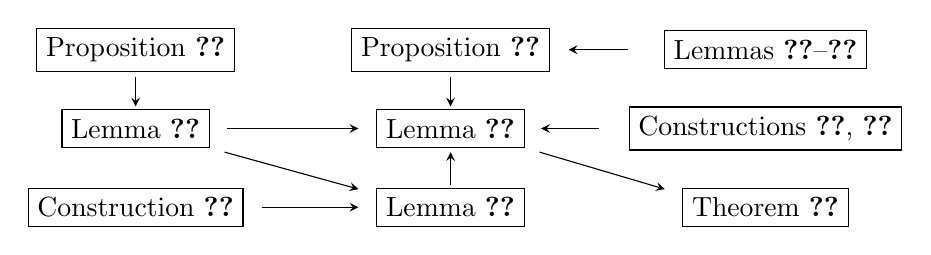
\begin{tikzpicture}
\node[draw,align=center] at (0,0)
{Proposition \ref{divlocal.9}};
\node[draw,align=center] at (4,0)
{Proposition \ref{lemma.7}};
\node[draw,align=center] at (8,0)
{Lemmas \ref{lemma.17}--\ref{lemma.12}};
\node[draw,align=center] at (0,-1)
{Lemma \ref{local.2}};
\node[draw,align=center] at (4,-1)
{Lemma \ref{local.4}};
\node[draw,align=center] at (8,-1)
{Constructions \ref{divlocal.2}, \ref{divlocal.11}};
\node[draw,align=center] at (0,-2)
{Construction \ref{divlocal.7}};
\node[draw,align=center] at (4,-2)
{Lemma \ref{local.3}};
\node[draw,align=center] at (8,-2)
{Theorem \ref{local.5}};
\draw [-stealth](0,-0.35) -- (0,-0.72);
\draw [-stealth](4,-0.35) -- (4,-0.72);
\draw [-stealth](4,-1.72) -- (4,-1.3);
\draw [-stealth](6.25,0) -- (5.5,0);
\draw [-stealth](5.88,-1) -- (5.15,-1);
\draw [-stealth](1.16,-1) -- (2.83,-1);
\draw [-stealth](1.6,-2) -- (2.83,-2);
\draw [-stealth](1.13,-1.3) -- (2.83,-1.77);
\draw [-stealth](5.13,-1.3) -- (6.72,-1.77);
\end{tikzpicture}
\]

In Subsection \ref{cohomology}, we explain how we extend cohomology theories of schemes to fs log schemes.


\subsection{Key comparison}
\label{key}
Throughout this subsection, we fix $B\in \Sch$ and an open subscheme $C$ of $\G_{m,B}$.
We also fix a motivic $\infty$-category $\sT$, i.e., an $\Sm$-premotivic $\infty$-category over $\Sch/B$ whose homotopy category is a motivic triangulated category in the sense of \cite[Definition 2.4.45]{CD19}.
For a stable $\infty$-category $\cC$, let $\map_{\cC}(-,-)$ denote the mapping spectrum.



If $P$ is a sharp saturated monoid, then $P^{\gp}$ is torsion free by \cite[Proposition I.1.3.5(2)]{Ogu}.

\begin{lem}
\label{mono.1}
Let $P$ be an fs monoid.
Then there is a non-canonical decomposition
\[
P
\simeq
P^*\oplus \ol{P}.
\]
\end{lem}
\begin{proof}
Let $\theta\colon P\to \ol{P}$ be the quotient homomorphism.
Since $\ol{P}^{\gp}$ is torsion free, there exists a section $\eta\colon \ol{P}^\gp\to P^\gp$ of $\theta^\gp$.
Let $p$ be an element of $\ol{P}$, and choose an element $p'\in P$ such that $\theta(p')=p$.
Then
\[
\theta^\gp\eta(p)=p=\theta^\gp(p'),
\]
so $\eta(p)-p'\in \ker \theta^\gp=P^*$.
Thus $\eta(p)\in P$.
This means $\eta(\ol{P})\subset P$, so $\eta$ induces a section of $\theta$.
Let
\[
\lambda\colon P^*\oplus \ol{P}\to P
\]
be the homomorphism sending $(x,y)\in P^*\oplus \ol{P}$ to $x+\eta(y)$.

If $\lambda(x,y)=\lambda(x',y')$, then $\eta(y)-\eta(y')\in P^*$.
This means $y-y'=\theta(\eta(y))-\theta(\eta(y'))=0$.
Hence we have $x=x'$, which shows that $\lambda$ is injective.
If $q\in P$, then $q-\eta(\theta(q))\in P^*$, and $\lambda$ maps $(q-\eta(\theta(q)),\theta(q))$ to $q$.
Hence $\lambda$ is surjective.
\end{proof}

\begin{df}
For an fs monoid $P$, let $P^\tor$ be the torsion subgroup of $P^*$.
We set $P^\tf:=P/P^\tor$.
Lemma \ref{mono.1} gives a non-canonical decomposition
\begin{equation}
P
\simeq
P^\tf \oplus P^\tor.
\end{equation}
\end{df}


\begin{lem}
\label{lemma.10}
Suppose $f\colon Y'\to Y$ is a dividing cover in $\lSm/X$, where $X\in \lSch$.
For all open immersions $U\to Y$ and $V\to Y-\partial Y$, there is a canonical equivalence
\[
\map_{\sT(\ul{U})}
(M(\ul{U}),M(V))
\simeq
\map_{\sT(\ul{U\times_Y Y'})}
(M(\ul{U\times_Y Y'}),M(V\times_Y Y')).
\]
\end{lem}
\begin{proof}
Let $g\colon \ul{U\times_Y Y'}\to \ul{U}$ be the projection.
Consider the induced cartesian square
\[
\begin{tikzcd}
V\times_Y Y'\ar[d,"\simeq"']\ar[r]&
\ul{U\times_Y Y'}\ar[d,"g"]
\\
V\ar[r]&
\ul{U}.
\end{tikzcd}
\]
We have equivalences
\[
g_*g^*M(V)
\simeq
g_*M(V\times_Y Y')
\simeq
M(V),
\]
where we use Theorem \ref{consq.1}(1) for the second equivalence.
By adjunction, we obtain the desired equivalence.
\end{proof}

\begin{const}
\label{lemma.11}
Recall that $C$ is an open subscheme of $\G_{m,B}$.
For $Y\in \lSch/\A_{\N,B}$ and integer $d$, we set
\[
\Phi_d(Y)
:=
\map_{\sT(\ul{Y})}
(M(\ul{Y})(d),M(Y\times_{\A_{\N,B}}C))
\in
\Ho(\Spt),
\]
which defines a functor $\Phi_d \colon (\lSch/\A_{\N,B})^{op}\to \Ho(\Spt)$.
We also set
\[
\Theta_d(Y)
:=
\Phi_d(Y-\partial_{\A_{\N,B}}Y).
\]
If $Y$ is vertical over $\A_{\N,B}$, then $\Theta_d(Y)\simeq \Phi_d(Y)$.

Suppose $f\colon Y'\to Y$ is a dividing cover in $\lSm/\A_{\N,B}$.
Lemma \ref{lemma.10} shows that $\Phi_d(f)$ is an isomorphism.
By Propositions \ref{vert.9}(1) and \ref{vert.8}, $(Y-\partial_{\A_{\N,B}}Y)\times_Y Y'$ is vertical over $\A_{\N,B}$.
In other words, we have the open immersion
\begin{equation}
\label{lemma.11.1}
(Y-\partial_{\A_{\N,B}}Y)\times_Y Y'
\hookrightarrow
Y'-\partial_{\A_{\N,B}} Y'.
\end{equation}
Hence we obtain a morphism
\begin{equation}
\label{lemma.11.2}
\Theta_d(f)\colon \Theta_d(Y')\to \Theta_d(Y)
\end{equation}
given by the composition
\[
\Phi_d(Y'-\partial_{\A_{\N,B}}Y')
\to 
\Phi_d((Y-\partial_{\A_{\N,B}}Y)\times_Y Y')
\simeq 
\Phi_d(Y-\partial_{\A_{\N,B}}Y).
\]
If $g\colon Y''\to Y'$ is another dividing cover, then use the commutative diagram
\[
\begin{tikzcd}[column sep=small, row sep=small]
(Y-\partial_{\A_{\N,B}}Y)\times_Y Y''\ar[r,hookrightarrow]\ar[d]&
(Y'-\partial_{\A_{\N,B}} Y')\times_{Y'}Y''\ar[r,hookrightarrow]\ar[d]&
Y''
\\
(Y-\partial_{\A_{\N,B}}Y)\times_Y Y'\ar[r,hookrightarrow]\ar[d]&
Y'-\partial_{\A_{\N,B}} Y'
\\
Y-\partial_{\A_{\N,B}}Y
\end{tikzcd}
\]
to show $\Theta_d(g)\Theta_d(f)\simeq \Theta_d(gf)$.
Hence $\Theta_d$ is covariant for dividing covers.
On the other hand, $\Theta_d$ is contravariant for open immersions.
\end{const}

\begin{prop}
\label{lemma.7}
For all dividing cover $p$ in $\lSm/\A_{\N,B}$ and integer $d$, $\Theta_d(p)$ is an isomorphism.
\end{prop}

Lemmas \ref{lemma.17}--\ref{lemma.12} are the steps of the proof.
We only write the case of $d=0$ for notational ease, and we set $\Phi:=\Phi_0$ and $\Theta:=\Theta_0$.
We finish the proof at the end of this section.

For an fs monoid $P$ and its ideal $I$, let $\A_{(P,I)}$ be the strict closed subscheme of $\A_P$ whose underlying scheme is given by $\Spec(\Z[P]/(I))$.
We set
\[
\A_{(P,I),B}:=\A_{(P,I)}\times B,
\;
\pt_{\N}:=\A_{(\N,\N^+)},
\;
\pt_{\N,B}:=\pt_{\N}\times B.
\]



\begin{lem}
\label{lemma.17}
Let $\theta\colon \N\to P$ be a vertical homomorphism of fs monoids.
Assume that $\ol{P}\simeq \N^n$ for some  integer $n\geq 1$.
If $F$ is a face of $P$ with $F\neq P$, then we have an isomorphism
\[
\Phi(\A_{P_F,B})
\simeq
\Phi(\A_{P,B}).
\]
\end{lem}
\begin{proof}
Replace $(P,B)$ by $(\ol{P},\A_{P^*,B})$ to reduce to the case when $P\simeq \N^n$.
We proceed by induction on $n$.
The claim is trivial for $n=1$.
Assume $n>1$.
By induction, we only need to consider the case when the rank of $F^\gp$ is $n-1$.
Let $\{e_1,\ldots,e_n\}$ be the standard coordinate in $\Z^n$.
Without loss of generality, we may assume that $F$ is generated by $e_2,\ldots,e_n$.


We express $\theta(1)$ as $(a_1,\ldots,a_n)$ with $a_1,\ldots,a_n >0$.
Let $L$ be the lattice for $\Spec(P)$.
We set
\begin{gather*}
Q:=((a_1e_1+a_2e_2)\Q\oplus (-e_1)\Q \oplus e_3\Q\cdots \oplus e_n \Q)\cap L^\vee,
\\
Q':=((a_1e_1+a_2e_2)\Q\oplus e_2\Q\oplus e_3\Q\cdots \oplus e_n \Q)\cap L^\vee.
\end{gather*}
We have the homomorphisms $\N\to Q,Q'$ induced by $\theta$.
The dual cones are
\begin{gather*}
\Spec(Q)=((-a_2e_1+a_1e_2)\Q \oplus e_2 \Q \oplus \cdots \oplus e_n \Q)\cap L,
\\
\Spec(Q')=((-a_2e_1+a_1e_2)\Q \oplus e_1 \Q\oplus e_3\Q\oplus \cdots \oplus e_n \Q)\cap L.
\end{gather*}
We have the face $G:=((a_1e_1+a_2e_2)\Q\oplus e_3\Q\cdots \oplus e_n \Q)\cap L^\vee$ of $Q$ and $Q'$.




By \cite[Proposition I.2.2.1]{Ogu}, there exists a homomorphism $\eta\colon Q\to \N$ such that $\eta^{-1}(0)=G$.
Consider the homomorphism $\mu\colon Q\to Q\oplus \N$ sending $\sigma\in Q$ to $(\sigma,\eta(\sigma))$, which induces a homomorphism
\[
h\colon \Z[Q]\to \Z[Q\oplus \N].
\]
The zero and one sections $\Spec(\Z)\rightrightarrows \A^1$ induce homomorphisms
\[
a_0,a_1\colon \Z[Q\oplus \N]
\to
\Z[Q].
\]
Consider the log structure homomorphism $\gamma\colon Q\oplus \N \to \Z[Q\oplus \N]$.
We set $x^\sigma:=\gamma(\sigma,0)$ for $\sigma\in Q$ and $t:=\gamma(0,1)$.
Then $a_1h=\id$ and
\[
a_0 h(x^\sigma)=a_0(x^\sigma t^{\eta(\sigma)})
=
\left\{
\begin{array}{ll}
0 & \text{if }\sigma\in Q-G,
\\
x^\sigma & \text{if }\sigma\in G.
\end{array}
\right.
\]
This shows that the induced morphism
\[
m\colon \ul{\A_Q}\times \A^1\to \ul{\A_Q}.
\]
is an elementary $\A^1$-homotopy between $ip$ and $\id$ over $\ul{\A_\N}$, where $p\colon \ul{\A_Q}\to \ul{\A_{G}}$ is the morphism induced by the inclusion $G\to Q$, and $i\colon \ul{\A_G}\simeq \ul{\A_{(Q,Q-G)}}\to \ul{\A_Q}$ is the obvious closed immersion.




Use $m$ to obtain an isomorphism
\begin{equation}
\label{lemma.17.1}
\Phi(\A_{Q,B})
\simeq
\Phi(\A_{G,B}).
\end{equation}
We can similarly show
\begin{equation}
\label{lemma.17.2}
\Phi(\A_{Q',B})
\simeq
\Phi(\A_{G,B}).
\end{equation}
Let $\Delta$ be the fan in $L$ whose maximal cones are $\Spec(P)$ and $\Spec(Q)$.
Then $\Delta$ is a subdivision of $\Spec(Q')$.
Hence we have
\begin{equation}
\label{lemma.17.3}
\Phi(\T_{\Delta,B})\simeq \Phi(\A_{Q',B}).
\end{equation}
The intersection of the cones $\Spec(P)$ and $\Spec(Q)$ is $\Spec(P_F)$.
By Zariski descent, the induced square
\[
\begin{tikzcd}
\Phi(\T_{\Delta,B})\ar[d]\ar[r]&
\Phi(\A_{Q,B})\ar[d]
\\
\Phi(\A_{P,B})\ar[r]&
\Phi(\A_{P_F,B})
\end{tikzcd}
\]
is cartesian.
Combine with \eqref{lemma.17.1}, \eqref{lemma.17.2}, and \eqref{lemma.17.3} to finish the proof.
\end{proof}

For every fan $\Sigma$ in a lattice $L$, let $|\Sigma|_{\R}$ denote the closure of the support $|\Sigma|$ in $\R\otimes_{\Q} L$.
The origin of $|\Sigma|_{\R}$ is denoted by $0$.

\begin{lem}
\label{lemma.16}
Let $\theta\colon \N\to P$ be a nontrivial homomorphism of fs monoids.
If $P^\gp$ is torsion tree and $P^+\neq 0$, then the topological space
\[
|\Spec(P)-\partial_{\Spec(\N)}\Spec(P)|_{\R}-\{0\}
\]
is acyclic.
\end{lem}
\begin{proof}
If $\theta$ is vertical, then
$|\Spec(P)-\partial_{\Spec(\N)}\Spec(P)|_{\R}-\{0\}=|\Spec(P)|_{\R}-\{0\}$ is contractible since $|\Spec(P)|_{\R}-\{0\}$ is convex.

Assume $\theta$ is not vertical.
Let $f\colon |\Spec(P)|_{\R}\to |\Spec(\N)|_{\R}\simeq \R_{\geq 0}$ be the map induced by $\theta$.
Choose any homomorphism $\eta\colon \N\to P$ such that $\eta(1)$ is not contained in any proper face of $P$.
This induces a map $h\colon |\Spec(P)|_{\R}\to \R_{\geq 0}$ such that $h^{-1}(0)=0$.
We set
\[
V:=f^{-1}(0)\cap h^{-1}(1)
\text{ and }
W:=|\Spec(P)-\partial_{\Spec(\N)}\Spec(P)|_{\R}\cap h^{-1}(1).
\]
For a cone $\sigma\in \Spec(P)$, we have $\sigma\in \Spec(P)-\partial_{\Spec(\N)}\Spec(P)$ if and only if $\sigma$ does not contain a ray $r$ with $f(r)=0$. 
Hence $f(x)>0$ for all $x\in |\Spec(P)-\partial_{\Spec(\N)}\Spec(P)|_{\R}-\{0\}$, so we have $V\cap W=\emptyset$.
There is a homeomorphism
\[
|\Spec(P)-\partial_{\Spec(\N)}\Spec(P)|_{\R}-\{0\}
\simeq
W\times \R_{>0}.
\]
Hence it suffices to show that $W$ is acyclic.

Let $X$ be the boundary of $h^{-1}(1)$.
Since $h^{-1}(1)$ is a convex polytope, $X$ is homeomorphic to $S^{n-2}$, where $n$ is the rank of $\ol{P}^\gp$.
We assumed that $\theta$ is not vertical, so we have $W\subset X$.
By the Alexander duality
\[
\tilde{H}_q(X-W)
\simeq
\tilde{H}^{n-q-3}(W)
\]
for all integer $q\geq 0$, we only need to show that $U:=X-W$ is acyclic.

Let $\Gamma$ be the set of cones $\sigma$ of $\Spec(P)$ such that there exists two rays $r_1$ and $r_2$ of $\sigma$ with $f(r_1)=0$ and $f(r_2)\neq 0$.
Equivalently, $|\sigma|_{\R}\cap V,|\sigma|_{\R}\cap W\neq \emptyset$.
We set $u(\sigma):=|\sigma|_{\R}\cap U$.
Let $\{\sigma_1,\ldots,\sigma_m\}$ be the set of elements of $\Gamma$.
Suppose $I:=\{i_1,\ldots,i_r\}$ is a nonempty subset of $\{1,\ldots,m\}$, and we set $\sigma_I:=\sigma_{i_1}\cap \cdots \cap \sigma_{i_r}$.
If $u(\sigma_I)=\emptyset$, then $u(\sigma_I)\cap V=\emptyset$.
On the other hand, if $u(\sigma_I)\neq \emptyset$, then $\sigma_I$ contains a ray $r$ with $f(r)=0$.
Hence we have $u(\sigma_I)\cap V\neq \emptyset$.
Since $u(\sigma_I)$ and $u(\sigma_I)\cap V$ are convex, they are contractible.
Hence the inclusion
\[
u(\sigma_I)\cap V
\to
u(\sigma_I)
\]
is a homotopy equivalence.

Since 
$\{u(\sigma_1),\ldots,u(\sigma_m),V\}$ (resp.\ $\{u(\sigma_1)\cap V,\ldots,u(\sigma_m)\cap V,V\}$) is a closed cover of $U$ (resp.\ $V$), the homomorphism of singular cohomology groups $H_*(V)\to H_*(U)$ induced by the inclusion $V\to U$ is an isomorphism by 
Mayer-Vietoris.
The assumption that $\theta$ is nontrivial implies that $V$ is not empty.
Furthermore, $V$ is convex, so $V$ is contractible.
It follows that $U$ is acyclic.
\end{proof}

\begin{exm}
Let us give a specific example for Lemma \ref{lemma.16} to help the readers to understand its proof.
Suppose $P$ is the submonoid of $\Z^3$ generated by $(1,0,0)$, $(0,1,0)$, $(1,0,1)$, $(0,1,1)$.
Then $|\Spec(P)|_{\R}$ is generated by $(1,0,0)$, $(0,1,0)$, $(0,0,1)$, and $(1,1,-1)$.
Suppose $\theta\colon \N\to P$ (resp.\ $\eta\colon \N\to P$) is the homomorphism sending $1$ to $(1,1,0)$ (resp.\ $(1,1,1)$).
Then $f$ (resp.\ $h$) sends $(x,y,z)$ to $x+y$ (resp.\ $x+y+z$).
The following figure illustrates several topological spaces appearing in the proof of Lemma \ref{lemma.16}.
\[
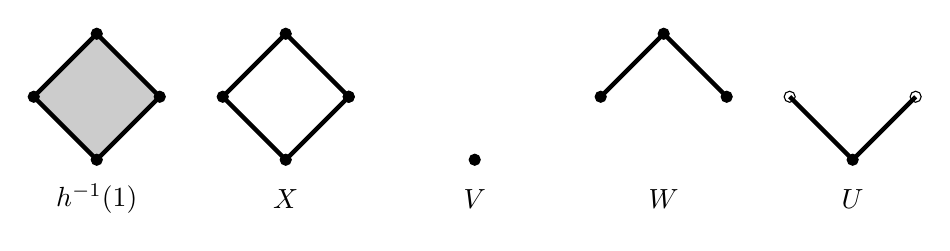
\begin{tikzpicture}
\fill[black!20] (0.8,0)--(0,0.8)--(-0.8,0)--(0,-0.8);
\draw[ultra thick] (0.8,0)--(0,0.8)--(-0.8,0)--(0,-0.8)--(0.8,0);
\filldraw (0.8,0) circle (2pt);
\filldraw (0,0.8) circle (2pt);
\filldraw (-0.8,0) circle (2pt);
\filldraw (0,-0.8) circle (2pt);
\node at (0,-1.3) {$h^{-1}(1)$};
\draw[ultra thick] (3.2,0)--(2.4,0.8)--(1.6,0)--(2.4,-0.8)--(3.2,0);
\filldraw (3.2,0) circle (2pt);
\filldraw (2.4,0.8) circle (2pt);
\filldraw (1.6,0) circle (2pt);
\filldraw (2.4,-0.8) circle (2pt);
\filldraw (3.2,0) circle (2pt);
\node at (2.4,-1.3) {$X$};
\filldraw (4.8,-0.8) circle (2pt);
\node at (4.8,-1.3) {$V$};
\draw[ultra thick] (8,0)--(7.2,0.8)--(6.4,0);
\filldraw (8,0) circle (2pt);
\filldraw (7.2,0.8) circle (2pt);
\filldraw (6.4,0) circle (2pt);
\node at (7.2,-1.3) {$W$};
\draw[ultra thick] (10.4,0)--(9.6,-0.8)--(8.8,0);
\draw (10.4,0) circle (2pt);
\filldraw (9.6,-0.8) circle (2pt);
\draw (8.8,0) circle (2pt);
\node at (9.6,-1.3) {$U$};
\end{tikzpicture}
\]

\end{exm}

\begin{lem}
\label{lemma.15}
Let $f\colon \Delta\to \Spec(\N)$ be a vertical morphism of fans, and let $\sigma$ be any nontrivial cone of $\Delta$.
If the topological space $|\Delta|_{\R}-\{0\}$ is acyclic, then there is an isomorphism $\Phi(\T_{\sigma,B})\simeq \Phi(\T_{\Delta,B})$.
\end{lem}
\begin{proof}
Since $\Phi$ is invariant for dividing covers, we may assume that every cone of $\Delta$ is smooth by \cite[Theorem 11.1.9]{CLStoric}.
For a cone $\delta$ of $\Delta$, we set
\[
\Phi(\delta)
:=
\Phi(\T_{\delta,B}).
\]
Observe that $\Phi$ is contravariant for the inclusions of cones.

There exists a colimit preserving functor
\[
\alpha\colon \Spt \to \sT(S)
\]
sending the sphere spectrum $\mathbb{S}$ to $\unit$ by \cite[Corollary 1.4.4.6]{HA}.
For a space $V$, we set
\[
\epsilon(V)
:=
\alpha(\map_{\Spt}(\Sigma^\infty V,\mathbb{S})).
\]
If $V$ is contractible, then $\epsilon(V)\simeq \unit$.
If $V$ is empty, then $\epsilon(V)\simeq 0$.

If $\delta'\subset \delta$ are nontrivial cones of $\Delta$, then Lemma \ref{lemma.17} shows $\Phi(\delta')\simeq \Phi(\delta)$.
Together with the connectivity of $|\delta|_{\R}-\{0\}$, we have
\[
\Phi(\delta)\simeq \Phi(\sigma).
\]
Observe also that $|\delta|_{\R}-\{0\}$ is contractible since it is convex.
On the other hand, $\Phi(\delta)=\Phi(0)$ if $\delta=0$.
These two formulas for $\Phi$ can be combined into a single functorial isomorphism
\begin{equation}
\label{lemma.15.3}
\Phi(\delta)
\simeq
\Phi(\sigma)\otimes \epsilon(|\delta|_{\R}-\{0\})
\oplus
\Phi(0)\otimes \fib(\unit \to \epsilon(|\delta|_{\R}-\{0\}))
\end{equation}
for all cone $\delta$ of $\Delta$.

Let $\delta_1,\ldots,\delta_m$ be all the maximal cones of $\Delta$.
If $v$ is an object of the simplicial set $I:=(\Delta^1)^m-\{(1,\ldots,1)\}$, we set
\[
\delta_v:=\delta_{i_1}\cap \cdots \cap \delta_{i_r},
\]
where the $i$-th coordinate of $v$ is $0$ if and only if $i\in \{i_1,\ldots,i_r\}$.
If $v\to w$ is a morphism in $I$, then we have the morphism $\delta_v\to \delta_w$ given by the inclusion of the cones.
Hence we can take limits on both sides of \eqref{lemma.15.3} to obtain an equivalence
\begin{equation}
\label{lemma.15.2}
\limit_{v\in I} \Phi(\delta)
\simeq
\limit_{v\in I}
\big(
\Phi(\sigma)\otimes \epsilon(|\delta|_{\R}-\{0\})
\oplus
\Phi(0)\otimes \fib(\unit \to \epsilon(|\delta|_{\R}-\{0\}))
\big).
\end{equation}
The left hand side of \eqref{lemma.15.2} is equivalent to $\Phi(\T_{\Delta,B})$ by Zariski descent.
Since $\{|\delta_1|_{\R}-\{0\},\ldots,|\delta_m|_{\R}-\{0\}\}$ is a closed cover of $|\Delta|_{\R}-\{0\}$, the right hand side of \eqref{lemma.15.2} is equivalent to
\[
\Phi(\sigma)\otimes \epsilon(|\Delta|_{\R}-\{0\})
\oplus
\Phi(0)\otimes \fib(\unit \to \epsilon(|\Delta|_{\R}-\{0\}))
\]
by Mayer-Vietoris, which is equivalent to $\Phi(\sigma)$ since $|\Delta|_{\R}-\{0\}$ is acyclic.
\end{proof}

We refer to \cite[Section 11.1]{CLStoric} for the definition of a star subdivision of a fan.

\begin{lem}
\label{lemma.1}
Let $\theta\colon \N\to Q$ be a homomorphism of fs monoids, and let $\Sigma$ be a star subdivision of $\Spec(P)$ with $P:=Q^\tf$.
Then $\Theta(p)$ is an isomorphism, where $p\colon \A_{Q,B}\times_{\A_P}\T_{\Sigma}\to \A_{Q,B}$ is the projection.
\end{lem}
\begin{proof}
Replace $(Q,B)$ by $(P,\A_{Q^\tor,B})$ to reduce to the case when $Q^\gp$ is torsion free, i.e., $P=Q$.

If $\theta$ is trivial, then
\[
\A_{P,B}-\partial_{\A_{\N,B}}\A_{P,B}
\simeq
\A_{P,B}-\partial\A_{P,B}
\simeq 
\T_{\Sigma,B}-\partial_{\A_{\N,B}}\T_{\Sigma,B}
\simeq
\T_{\Sigma,B}-\partial\T_{\Sigma,B}.
\]
Hence $\Theta(p)$ is an isomorphism.

Assume $\theta$ is nontrivial.
Let $N$ be the dual lattice of $P^\gp$, and let $v$ be the point of $|\Spec(P)|\cap N$ such that $\Sigma$ is the star subdivision of $\Spec(P)$ at $v$.
If $f(v)=0$, then $\Sigma-\partial_{\Spec(\N)}\Sigma\simeq \Spec(P)-\partial_{\Spec(\N)}\Spec(P)$.
Hence we are done.

Assume $f(v)\neq 0$.
For every $x\in |\Sigma-\partial_{\Spec(\N)}\Sigma|_{\R}$, the segment whose two ends are $x$ and $v$ is contained in $|\Sigma-\partial_{\Spec(\N)}\Sigma|_{\R}$.
It follows that $|\Sigma-\partial_{\Spec(\N)}\Sigma|_{\R}-\{0\}$ is contractible.
Together with Lemmas \ref{lemma.16} and \ref{lemma.15}, we obtain $\Theta(\A_P)\simeq \Theta(\T_\Sigma)$.
\end{proof}




\begin{lem}
\label{lemma.8}
Let $\theta\colon \N\to Q$ be a homomorphism of fs monoids, let $X\to \A_{Q,B}$ be a strict \'etale morphism in $\lSch$, and let $\Sigma$ be a star subdivision of $\Spec(P)$ with $P:=Q^\tf$.
Then $\Theta(p)$ is an isomorphism, where $p\colon X':=X\times_{\A_P}\T_{\Sigma}\to X$ is the projection.
\end{lem}
\begin{proof}
We proceed by induction on $m:=\rank(\ol{P}^\gp)$.
If $m=0,1$, then there is no nontrivial star subdivision of $\Spec(P)$.
Hence the claim is trivial.

Assume $m\geq 2$.
Let $i\colon \A_{(P,P^+),B}\to \A_{P,B}$ be the obvious closed immersion, let $j$ be its open complement, and let $q\colon \T_\Sigma\to \A_P$ be the projection.
We have the induced commutative diagram with cartesian squares
\begin{equation}
\label{lemma.8.1}
\begin{tikzcd}
\A_{(P,P^+),B}\times_{\A_P}\T_{\Sigma,B}\ar[d]\ar[r,"i'"]&
\T_{\Sigma,B}\ar[d,"q"]\ar[r,leftarrow,"j'"]&
(\A_{P,B}-\A_{(P,P^+),B})\times_{\A_P}\T_\Sigma\ar[d]
\\
\A_{(P,P^+),B}\ar[r,"i"]&
\A_{P,B}\ar[r,leftarrow,"j"]&
\A_{P,B}-\A_{(P,P^+),B}.
\end{tikzcd}
\end{equation}

Consider the morphism $\A_{P,B}\to \ul{ \A_{(P,P^+),B}}\simeq \A_{P^*,B}$ induced by the inclusion $P^*\to P$.
We set
\[
Y:=\ul{X\times_{\A_{P,B}} \A_{(P,P^+),B}}\times_{\ul{\A_{(P,P^+),B}}}\A_{P,B},
\;
Y':=\ul{X\times_{\A_{P,B}} \A_{(P,P^+),B}}\times_{\ul{\A_{(P,P^+),B}}}\T_{\Sigma,B}.
\]
Since $X$ is strict smooth over $\A_{P,B}$, $Y$ (resp.\ $Y'$) is strict smooth over $\A_{P,B}$ (resp.\ $\T_{\Sigma,B}$).
There is a commutative diagram with cartesian squares
\begin{equation}
\label{lemma.8.2}
\begin{tikzcd}[column sep=small, row sep=small]
X'\ar[r,leftarrow]\ar[d]&
X'\times_{\A_{P,B}}\A_{(P,P^+),B}\ar[r]\ar[d]&
Y'\ar[d]
\\
X\ar[r,leftarrow]\ar[d]&
X\times_{\A_{P,B}}\A_{(P,P^+),B}\ar[d]\ar[r]&
Y\ar[d]
\\
\A_{P,B}\ar[r,leftarrow,"i"]&
\A_{(P,P^+),B}\ar[r,"i"]&
\A_{P,B}.
\end{tikzcd}
\end{equation}


For simplicity of notation, we set $U:=C\times_{\A_{\N}}\A_P$ and $U':=U\times_{\A_P}\T_{\Sigma}\simeq U$.
By Theorem \ref{consq.1}, we have an equivalence $\ul{q}_*M(U')\simeq M(U)$.
Since $q$ is log smooth, there is a commutative diagram
\begin{equation}
\label{lemma.2.3}
\begin{tikzcd}
\ul{q}^*\ul{j}_\sharp \ul{j}^*\ar[r,"ad'"]\ar[d,"\simeq"']&
\ul{q}^*\ar[r,"ad"]\ar[d,"\simeq"]&
\ul{q}^*\ul{i}_*\ul{i}^*\ar[d,"\simeq"]
\\
\ul{j}_\sharp'\ul{j}'^*\ul{q}^*\ar[r,"ad'"]&
\ul{q}'^*\ar[r,"ad"]&
\ul{i}_*'\ul{i}'^*\ul{q}^*
\end{tikzcd}
\end{equation}
whose rows are cofiber sequences and vertical maps are equivalences.
We set $Y'':=(Y-\partial_{\A_{\N,B}}Y)\times_Y Y'$.
From \eqref{lemma.2.3}, we obtain a commutative diagram
\[
\begin{tikzcd}[row sep=small, column sep=tiny]
\map_{\sT(\ul{\T_{\Sigma,B}})}(\ul{i}_*'\ul{i}'^*M(\ul{Y''}),M(U'))\ar[d]\ar[r,"\simeq"]&
\map_{\sT(\ul{\A_{P,B}})}(\ul{i}_*\ul{i}^*M(\ul{Y-\partial_{\A_{\N,B}}Y}),M(U))\ar[d]
\\
\map_{\sT(\ul{\T_{\Sigma,B}})}(M(\ul{Y''}),M(U'))\ar[d]\ar[r,"\simeq"]&
\map_{\sT(\ul{\A_{P,B}})}(M(\ul{Y-\partial_{\A_{\N,B}}Y}),M(U))\ar[d]
\\
\map_{\sT(\ul{\T_{\Sigma,B}})}(\ul{j}_\sharp' \ul{j}'^*M(\ul{Y''}),M(U'))\ar[r,"\simeq"]&
\map_{\sT(\ul{\A_{P,B}})}(\ul{j}_\sharp\ul{j}^*M(\ul{Y-\partial_{\A_{\N,B}}Y}),M(U))
\end{tikzcd}
\]
whose columns are fiber sequences.
Together with the open immersion $Y''\hookrightarrow Y'-\partial_{\A_{\N,B}}Y'$, we obtain a commutative diagram
\begin{equation}
\label{lemma.2.1}
\begin{tikzpicture}[baseline= (a).base]
\node[scale=.9] (a) at (0,0)
{
\begin{tikzcd}[row sep=small, column sep=tiny]
\map_{\sT(\ul{\T_{\Sigma,B}})}(\ul{i}_*'\ul{i}'^*M(\ul{Y'-\partial_{\A_{\N,B}}Y'}),M(U'))\ar[d]\ar[r]&
\map_{\sT(\ul{\A_{P,B}})}(\ul{i}_*\ul{i}^*M(\ul{Y-\partial_{\A_{\N,B}}Y}),M(U))\ar[d]
\\
\map_{\sT(\ul{\T_{\Sigma,B}})}(M(\ul{Y'-\partial_{\A_{\N,B}}Y'}),M(U'))\ar[d]\ar[r]&
\map_{\sT(\ul{\A_{P,B}})}(M(\ul{Y-\partial_{\A_{\N,B}}Y}),M(U))\ar[d]
\\
\map_{\sT(\ul{\T_{\Sigma,B}})}(\ul{j}_\sharp' \ul{j}'^*M(\ul{Y'-\partial_{\A_{\N,B}}Y'}),M(U'))\ar[r]&
\map_{\sT(\ul{\A_{P,B}})}(\ul{j}_\sharp\ul{j}^*M(\ul{Y-\partial_{\A_{\N,B}}Y}),M(U))
\end{tikzcd}
};
\end{tikzpicture}
\end{equation}
whose columns are fiber sequences.

The fs log scheme $\A_{P,B}-\A_{(P,P^+),B}$ admits a Zariski cover
\[
\{\A_{P_F,B}:
F\text{ is a nonzero face of }P\}.
\]
By induction, the morphism $\Theta(Y'\times_{\A_P}\A_{P_F})\to \Theta(Y\times_{\A_P}\A_{P_F})$ is an isomorphism.
Hence by Zariski descent and adjunction, the third row of \eqref{lemma.2.1} is an equivalence.

Lemma \ref{mono.1} gives isomorphisms
\[
Y:=\ul{X\times_{\A_{P,B}} \A_{(P,P^+),B}}\times \A_{\ol{P},B},
\;
Y':=\ul{X\times_{\A_{P,B}} \A_{(P,P^+),B}}\times \T_{\Sigma',B},
\]
where $\Sigma':=\Sigma\times_{\Spec(P)}\Spec(\ol{P})$ is a star subdivision of $\Spec(\ol{P})$.
Replace $B$ by $\ul{X\times_{\A_{P,B}} \A_{(P,P^+),B}}$ and use Lemma \ref{lemma.1} to deduce that the second row of \eqref{lemma.2.1} is an equivalence.
It follows that the first row of \eqref{lemma.2.1} is an equivalence too.




We also have a commutative diagram
\begin{equation}
\label{lemma.2.2}
\begin{tikzpicture}[baseline= (a).base]
\node[scale=.9] (a) at (0,0)
{
\begin{tikzcd}[row sep=small, column sep=tiny]
\map_{\sT(\ul{\T_{\Sigma,B}})}(\ul{i}_*'\ul{i}'^*M(\ul{X'-\partial_{\A_{\N,B}}X'}),M(U'))\ar[d]\ar[r]&
\map_{\sT(\ul{\A_{P,B}})}(\ul{i}_*\ul{i}^*M(\ul{X-\partial_{\A_{\N,B}}X}),M(U))\ar[d]
\\
\map_{\sT(\ul{\T_{\Sigma,B}})}(M(\ul{X'-\partial_{\A_{\N,B}}X'}),M(U'))\ar[d]\ar[r]&
\map_{\sT(\ul{\A_{P,B}})}(M(\ul{X-\partial_{\A_{\N,B}}X}),M(U))\ar[d]
\\
\map_{\sT(\ul{\T_{\Sigma,B}})}(\ul{j}_\sharp' \ul{j}'^*M(\ul{X'-\partial_{\A_{\N,B}}X'}),M(U'))\ar[r]&
\map_{\sT(\ul{\A_{P,B}})}(\ul{j}_\sharp\ul{j}^*M(\ul{X-\partial_{\A_{\N,B}}X}),M(U))
\end{tikzcd}
};
\end{tikzpicture}
\end{equation}
whose rows are fiber sequences.
From \eqref{lemma.8.2}, we see that the first rows of \eqref{lemma.2.1} and \eqref{lemma.2.2} are equivalent.
By induction, the morphism $\Theta(X'\times_{\A_P}\A_{P_F})\to \Theta(X\times_{\A_P}\A_{P_F})$ is an isomorphism for every nonzero face $F$ of $P$.
Hence by Zariski descent and adjunction, the third row of \eqref{lemma.2.2} is an equivalence.
It follows that the second row of \eqref{lemma.2.2} is an equivalence too.
By adjunction, we obtain the desired equivalence.
\end{proof}



\begin{lem}
\label{lemma.14}
Let $\theta\colon \N\to Q$ be a homomorphism of fs monoids, let $X\to \A_{Q,B}$ be a strict \'etale morphism, let $\Sigma$ be a subdivision of $\Spec(P)$ with $P:=Q^\tf$, and let $\Delta$ be a subdivision of $\Sigma$ obtained by finite successions of star subdivisions.
Then $\Theta(q)$ is an isomorphism, where $q\colon X\times_{\A_{P}}\T_{\Delta}\to X\times_{\A_{P}}\T_{\Sigma}$ be the induced morphism.
\end{lem}
\begin{proof}
We only need to show the claim when $\Delta$ is a star subdivision of $\Sigma$.
By Zariski descent, we reduce to the case when $\Sigma= \Spec(R)$ for an fs monoid $R$.
Then $X\times_{\A_P}\A_R\simeq X\times_{\A_Q}\A_{R\oplus Q^\tor}$ is strict \'etale over $\A_{R\oplus Q^\tor,B}$.
We can use Lemma \ref{lemma.8} in this situation.
\end{proof}

\begin{lem}
\label{lemma.13}
Let $\theta\colon \N\to Q$ be a homomorphism of fs monoids, let $X\to \A_{Q,B}$ be a strict \'etale morphism in $\lSch$, and let $\Sigma$ be a subdivision of $\Spec(P)$ with $P:=Q^\tf$.
Then $\Theta(p)$ is an isomorphism, where $p\colon X\times_{\A_{P}}\T_{\Sigma}\to X$ is the projection.
\end{lem}
\begin{proof}
Let $\cB$ be the category of subdivisions of $\Spec(P)$, and let $\cA$ be the class of morphisms in $\cA$ that are obtained by finite successions of star subdivisions relative to two dimensional cones.
By \cite[Lemma A.3.15]{logDM}, $\cA$ admits a calculus of right fractions in $\cB$.

Consider the functor
\[
F\colon \cB\to \Ho(\Spt).
\]
sending $\Sigma\in \cB$ to $\Theta(X\times_{\A_{P}}\T_{\Sigma})$.
By Lemma \ref{lemma.14}, $\Theta$ sends every morphism in $\cA$ to an isomorphism.
Together with \cite[Lemmas A.3.15, C.2.1]{logDM}, we deduce that $\Theta$ sends every morphism in $\cB$ to an isomorphism.
\end{proof}


\begin{lem}
\label{lemma.12}
Let $\N\to Q$ be a homomorphism of fs monoids, let $X\to \A_{Q,B}$ be a strict \'etale morphism in $\lSch$, let $X'\to X$ be a log \'etale monomorphism, and let $\Sigma$ be a subdivision of $\Spec(P)$ with $P:=Q^\tf$.
Then $\Theta(p)$ is an isomorphism, where $p\colon X'\times_{\A_{P}}\T_{\Sigma}\to X'$ is the projection.
\end{lem}
\begin{proof}
The question is Zariski local on $X$.
Hence by \cite[Lemma A.11.3]{logDM}, we may assume that there exists a homomorphism $\theta\colon P\to P'$ such that $\theta^\gp$ is an isomorphism and the induced morphism $X'\to X\times_{\A_P}\A_{P'}$ is an open immersion.
This means that the induced morphism $X'\to \A_{P'\oplus Q^{\tor},B}$ is strict \'etale.

We set $\Sigma':=\Spec(P')\times_{\Spec(P)}\Sigma$, which is a subdivision of $\Spec(P')$.
Then $X'\times_{\A_{P}}\T_{\Sigma}\simeq X'\times_{\A_{P'}}\T_{\Sigma'}$, and use Lemma \ref{lemma.13} to conclude.
\end{proof}




\begin{proof}[Proof of Proposition \ref{lemma.7}]
Let $f\colon X'\to X$ be a dividing cover in $\lSm/\A_{\N,B}$, and let $x$ be a point of $X$.
The question is Zariski local on $X$.
Since $X\in \lSm/B$, we may assume that there exists a neat chart $P$ of $X$ at $x$ such that the induced morphism $X\to \A_{P,B}$ is strict smooth by \cite[Lemma A.5.9]{logDM}.
We may also assume that this factors through a strict \'etale morphism $X\to \A_{P\oplus \Z^n,B}$ for some integer $n\geq 0$ by \cite[Corollaire IV.17.11.4]{SGA4}.
The morphism $X\to \A_{\N,B}$ induces a homomorphism $\eta\colon \N \to \ol{\cM}_{X,x}\simeq P$.
We set $Q:=P\oplus \Z^n$, and let $\theta\colon \N\to Q$ be the homomorphism given by $a\mapsto (\eta(a),0)$.

Due to \cite[Proposition A.11.5]{logDM}, there exists a subdivision $\Sigma$ of $\Spec(Q)$ such that the pullback
\[
r\colon X'\times_{\A_Q}\T_{\Sigma}\to X\times_{\A_Q}\T_{\Sigma}
\]
is an isomorphism.
Let $p\colon X\times_{\A_Q}\T_\Sigma\to X$ and $p'\colon X'\times_{\A_Q}\T_\Sigma\to X'$ be the projections.
By Lemma \ref{lemma.12}, $\Theta(p)$ and $\Theta(p')$ are isomorphisms.
Since $\Theta(r)\Theta(p)=\Theta(p')\Theta(f)$, $\Theta(f)$ is an isomorphism.
\end{proof}

\subsection{Localization functors}
\label{localization}

Throughout this subsection, $S\in \lSch$.
Furthermore, $\cV$ is either $\Spt$ or $\DLambda$.

Suppose $\cC$ is a category.
We set
\[
h(X)
:=
\left\{
\begin{array}{ll}
\Sigma_{S^1}^\infty X_+ & \text{if }\cV=\Spt,
\\
\Lambda^X[0] & \text{if }\cV=\DLambda
\end{array}
\right.
\]
for $X\in \cC$, which is an object of $\infPsh(\cC,\cV)$.
We set $h_t(X):=L_t h(x)$.
This defines a functor
\[
h_t\colon \Nerve(\cC) \to \infShv_t(\cC,\cV).
\]








\begin{df}
A \emph{fan chart} of an fs log scheme $X$ is a strict morphism $X\to \T_{\Sigma}$, where $\Sigma$ is a fan.
Let $\lFan$ denote the full subcategory of $\lSch$ consisting of disjoint unions $\amalg_{i\in I} X_i$ such that each $X_i$ has a fan chart.
Let $\lSmFan$ be the class of smooth morphisms $Y\to X$ with $Y\in \lFan$. 

For $X\in \lSch$, let $X_{div}$ be the full subcategory of $\lSch$ consisting of $Y$ such that $Y\to X$ is a dividing cover.

For a fan $\Sigma$, let $\Sigma_{div}$ be the category of subdivisions of $\Sigma$.
\end{df}

Every $X\in \lSm/S$ admits a Zariski cover $Y\to X$ with $Y\in \lSmFan/S$ according to \cite[Proposition II.2.3.7]{Ogu}.
Hence for every topology $t$ finer than the Zariski topology, we have an equivalence of topoi
\[
\Shv_t(\lSm/S)
\simeq
\Shv_t(\lSmFan/S)
\]
by the implication (i)$\Rightarrow$(ii) in \cite[Th\'eor\`eme III.4.1]{SGA4}.
This implies that we have an equivalence of $\infty$-categories
\begin{equation}
\infShv_t(\lSm/S,\cU)
\simeq
\infShv_t(\lSmFan/S,\cU)
\end{equation}
for $\cU=\Spc,\Spc_*,\Spt,\DLambda$.

\begin{lem}
\label{divlocal.10}
Suppose $X\in \lSch$.
\begin{enumerate}
\item[{\rm (1)}]
$X_{div}$ is filtered.
\item[{\rm (2)}]
If $X$ admits a fan chart $\Sigma$, then the functor
\[
\Sigma_{div}\to X_{div}
\]
sending $\Sigma'\in \Sigma_{div}$ to $X\times_{\T_\Sigma}\T_{\Sigma'}$ is final.
\item[{\rm (3)}]
For every dividing cover $f\colon Y\to X$ in $\lSch$, the functor $f^*\colon X_{div}\to Y_{div}$ is final.
\end{enumerate}
\end{lem}
\begin{proof}
By \cite[Proposition A.11.14]{logDM}, we have (1).
Use \cite[Proposition A.11.5]{logDM} to show (2).
For (3), suppose $Y'\in Y_{div}$.
Then $Y'\times_X Y\simeq Y'$ since $Y\to X$ is a monomorphism.
This shows that $f^*$ is final.
\end{proof}

\begin{prop}
\label{divlocal.12}
Let $f\colon Y\to X$ be a quasi-compact morphism in $\lSch$.
If $X$ admits a fan chart $\Sigma$, then there exists a subdivision $\Sigma'$ of $\Sigma$ such that the pullback
\[
f_\Sigma\colon Y\times_{\T_\Sigma}\T_{\Sigma'}\to X\times_{\T_\Sigma}\T_{\Sigma'}
\]
is exact.
\end{prop}
\begin{proof}
Choose a Zariski cover $Y_1\amalg \cdots \amalg Y_n$ of $Y$ such that each $Y_i\to X$ admits a fan chart $\Delta_i\to \Sigma$.
According to the proof of \cite[Theorem III.2.6.7]{Ogu} and the implication (1)$\Rightarrow$(2) in \cite[Theorem III.2.2.7]{Ogu}, there exists a subdivision $\Sigma_i$ of $\Sigma$ such that the pullback
\[
Y_i\times_{\T_{\Sigma}}\T_{\Sigma_i}
\to
X\times_{\T_{\Sigma}}\T_{\Sigma_i}
\]
is exact.
We set
\[
\Sigma'
:=
\{\sigma_1\cap \cdots \cap \sigma_n
:
\sigma_1\in \Sigma_1,\ldots,\sigma_n\in \Sigma_n\},
\]
which is a common subdivision of $\Sigma_1,\ldots,\Sigma_n$.
Then the pullback $Y_i\times_{\T_{\Sigma}}\T_{\Sigma'}\to X\times_{\T_{\Sigma}}\T_{\Sigma'}$ is exact for all $1\leq i\leq n$.
This implies that $f'$ is exact.
\end{proof}

\begin{prop}
\label{divlocal.8}
Suppose $\cF\in \infShv_{sNis}(\lSm/S,\cV)$.
Then $\cF$ is $dNis$-local if and only if $\cF(X)\to \cF(X')$ is an equivalence for all dividing cover $X'\to X$ in $\lSmFan/S$.
\end{prop}
\begin{proof}
Suppose $\cV=\DLambda$.
Then $\cF$ is $dNis$-local if and only if $\cF(X)\to \cF(X')$ is an equivalence for all dividing cover $X'\to X$ in $\lSm/S$ by \cite[Proposition 3.3.30, Corollary 3.4.11]{logDM}.
We conclude by Zariski descent.

If $\cV=\Spt$, argue similarly, but replace the reference \cite[Theorem 3.7]{MR2415380} in the proof of \cite[Corollary 3.4.11]{logDM} by \cite[Theorem 3.4]{MR2415380}.
\end{proof}


\begin{const}
\label{divlocal.7}
Consider the functor
\[
G_{div}\colon \infPsh(\lSmFan/S,\cV)
\to
\infPsh(\lSmFan/S,\cV)
\]
given by
\begin{equation}
\label{divlocal.7.1}
G_{div}\cF(X)
:=
\colimit_{X'\in X_{div}}\cF(X').
\end{equation}
If $X$ admits a fan chart $\Sigma$, then
\begin{equation}
G_{div}\cF(X)
\simeq
\colimit_{\Sigma'\in \Sigma_{div}}\cF(X_{\Sigma'})
\end{equation}
by Lemma \ref{divlocal.10}(2), where $X_{\Sigma'}:=X\times_{\T_\Sigma}\T_{\Sigma'}$.

Suppose $X\in \lSmFan/S$ has a fan chart $\Sigma$ and
\begin{equation}
\label{divlocal.7.2}
Q
:=
\begin{tikzcd}
W\ar[d]\ar[r]&
Z\ar[d]
\\
Y\ar[r]&
X
\end{tikzcd}
\end{equation}
is a strict Nisnevich distinguished square in $\lSmFan/S$.
For a subdivision $\Sigma'$ of $\Sigma$, we set
\[
X_{\Sigma'}:=X\times_{\T_{\Sigma}}\T_{\Sigma'},
\;
Y_{\Sigma'}:=Y\times_{\T_{\Sigma}}\T_{\Sigma'},
\;
Z_{\Sigma'}:=Z\times_{\T_{\Sigma}}\T_{\Sigma'},
\;
W_{\Sigma'}:=W\times_{\T_{\Sigma}}\T_{\Sigma'}.
\]
The induced square
\[
\begin{tikzcd}
W_{\Sigma'}\ar[d]\ar[r]&
Z_{\Sigma'}\ar[d]
\\
Y_{\Sigma'}\ar[r]&
X_{\Sigma'}
\end{tikzcd}
\]
is a strict Nisnevich distinguished square.
Hence the above $G_{div}$ induces 
\[
G_{div}
\colon
\infShv_{sNis}(\lSm/S,\cV)
\to
\infShv_{sNis}(\lSm/S,\cV).
\]
By Lemma \ref{divlocal.10}(3) and Proposition \ref{divlocal.8}, $\infShv_{dNis}(\lSm/S,\cV)$ is equivalent to the essential image of $G_{div}$.

There is a natural transformation $\beta_{div}\colon \id \to G_{div}$ such that the map
\[
\beta_{div}\cF(X) \colon \cF(X)\to \colimit_{X'\in X_{div}}\cF(X')
\]
for $\cF\in \infShv_{sNis}(\lSm/S,\cV)$ is induced by the maps $\cF(X)\to \cF(X')$ for all $X'\in X_{div}$.
Together with the description
\[
G_{div}G_{div}\cF(X)
\simeq
\colimit_{X'\in X_{div},X''\in X_{div}'}\cF(X''),
\]
we deduce that the two maps
\[
G_{div}\beta_{div}\cF,\beta_{div}G_{div}\cF
\colon
G_{div}\cF\to G_{div}G_{div}\cF
\]
are equivalences.
Hence by \cite[Proposition 5.2.7.4]{HTT}, $G_{div}$ is equivalent to $\iota_{div} L_{div}$, where  
\[
L_{div}
\colon
\infShv_{sNis}(\lSm/S,\cV)
\to
\infShv_{dNis}(\lSm/S,\cV).
\]
is the localization functor, and $\iota_{div}$ is the inclusion functor.
\end{const}

\begin{const}
\label{divlocal.2}
Suppose $f\colon X'\to X$ is a dividing cover in $\lSch/S$.
Consider the induced morphisms
\[
X-\partial_S X
\leftarrow
(X-\partial_S X)\times_S X'
\hookrightarrow
X'-\partial_S X'
\]
The left morphism becomes an isomorphism in the category of dividing Nisnevich sheaves.
Hence we obtain a morphism
\[
h_{dNis}(X-\partial_S X)
\to
h_{dNis}(X'-\partial_S X').
\]
Now, suppose $X\in \lFan/S$.
The \emph{dividing verticalization of $X$ over $S$} is defined to be
\begin{equation}
\label{divlocal.2.8}
h_{dver}(X)
:=
\colimit_{X'\in X_{div}^{op}}
h_{dNis}(X'-\partial_S X'),
\end{equation}
where the colimit is taken in the category of dividing Nisnevich sheaves.
If $X$ admits a fan chart $\Sigma$, then we have an isomorphism
\begin{equation}
h_{dver}(X)
\simeq
\colimit_{\Sigma'\in \Sigma_{div}^{op}}
h_{dNis}(X_{\Sigma'}-\partial_S X_{\Sigma'})
\end{equation}
by Lemma \ref{divlocal.10}(2), where $X_{\Sigma'}:=X\times_{\T_\Sigma}\T_{\Sigma'}$.

If $f\colon Y\to X$ is a morphism in $\lFan$, then there exists $X'\in X_{div}$ such that the projection $Y':=Y\times_X X'\to X'$ is exact by Proposition \ref{divlocal.12}.
For every $X''\in X_{div}'$ with $Y'':=Y\times_X X''$, we have the induced morphism
\[
Y''-\partial_S Y''\to X''-\partial_S X''
\]
by Proposition \ref{vert.9}(6).
Hence we obtain a morphism $h_{dver}(Y')\to h_{dver}(X')$.
Since $h_{dver}(X)\simeq h_{dver}(X')$ and $h_{dver}(Y)\simeq h_{dver}(Y')$ by Lemma \ref{divlocal.10}(3), we obtain a morphism $h_{dver}(Y)\to h_{dver}(X)$.
As a consequence, we obtain a functor
\[
h_{dver}
\colon
\lSmFan/S
\to
\infShv_{dNis}(\lSm/S,\cV).
\]
Take colimits to the morphisms $h_{dNis}(X'-\partial_S X')\to h_{dNis}(X')\simeq h_{dNis}(X)$ induced by the open immersion $X'-\partial_S X'\to X'$ for $X'\in X_{div}$ to obtain a natural transformation
\begin{equation}
\label{divlocal.2.5}
\alpha_{dver}\colon h_{dver}\to h_{dNis}.
\end{equation}
By \cite[Theorem 5.1.5.6]{HTT}, $h_{dver}$ naturally extends to a colimit preserving functor
\begin{equation}
\label{divlocal.2.1}
\infPsh(\lSmFan/S,\cV)
\to
\infShv_{dNis}(\lSm/S,\cV).
\end{equation}
\end{const}

\begin{const}
\label{divlocal.11}
Suppose $X\in \lSmFan/S$ has a fan chart $\Sigma$ with a strict Nisnevich distinguished square $Q$ of the form \eqref{divlocal.7.2}.
For a subdivision $\Sigma'$ of $\Sigma$, consider $X_{\Sigma'}$, $Y_{\Sigma'}$, $Z_{\Sigma'}$, and $W_{\Sigma'}$ in Construction \ref{divlocal.7}.

The induced square
\[
\begin{tikzcd}
W_{\Sigma'}-\partial_S W_{\Sigma'}\ar[d]\ar[r]&
Z_{\Sigma'}-\partial_S Z_{\Sigma'}\ar[d]
\\
Y_{\Sigma'}-\partial_S Y_{\Sigma'}\ar[r]&
X_{\Sigma'}-\partial_S X_{\Sigma'}
\end{tikzcd}
\]
is a strict Nisnevich distinguished square.
It follows that the square $h_{dver}(Q)$ is cocartesian in $\infShv_{sNis}(\lSm/S,\cV)$.

Suppose $X'\to X$ is a dividing cover in $\lSmFan/S$.
Since $X_{div}\to X_{div}'$ is final by Lemma \ref{divlocal.10}(3), the induced morphism
\[
h_{dver}(X')
\to
h_{dver}(X)
\]
is an equivalence.

Together with \cite[Proposition 5.5.4.20]{HTT}, we deduce that \eqref{divlocal.2.1} factors through a colimit preserving functor
\begin{equation}
\label{divlocal.2.2}
F_{dver}
\colon
\infShv_{dNis}(\lSm/S,\cV)
\to
\infShv_{dNis}(\lSm/S,\cV).
\end{equation}
This sends $h_{dNis}(X)$ for $X\in \lSmFan/S$ to $h_{dver}(X)$.
The natural transformation $\alpha_{dver}$ gives a natural transformation
\begin{equation}
\beta_{dver}
\colon
F_{dver} \to \id.
\end{equation}

For $X\in \lSmFan/S$ and $X'\in X_{div}$, the map
\[
F_{dver}(h_{dNis}(X'-\partial_S X'))
\to
h_{dNis}(X'-\partial_S X')
\]
induced by $\beta_{dver}$ is an equivalence since $X'-\partial_S X'$ is already vertical over $S$.
Take colimits to see that 
\[
\beta_{dver}h_{dver}(X)
\colon
F_{dver}h_{dver}(X)\to h_{dver}(X)
\]
is an equivalence.
Together with \cite[Theorem 5.1.5.6, Proposition 5.5.4.20]{HTT}, we deduce that
\begin{equation}
\label{divlocal.2.6}
\beta_{dver}F_{dver}(X)
\colon
F_{dver}F_{dver}(X)\to F_{dver}(X)
\end{equation}
is an equivalence.
There is a commutative triangle
\[
\begin{tikzcd}
F_{dver}h_{dver}(X)\ar[rd,"\beta_{dver}h_{dver}(X)"']\ar[rr,"F_{dver}\alpha_{dver}(X)"]&
&
F_{dver}h_{dNis}(X)\ar[ld,"\simeq",leftarrow]
\\
&
h_{dver}(X).
\end{tikzcd}
\]
Hence $F_{dver}\alpha_{dver}(X)$ is an equivalence.
Together with \cite[Theorem 5.1.5.6, Proposition 5.5.4.20]{HTT}, we deduce that
\begin{equation}
\label{divlocal.2.7}
F_{dver}\beta_{dver}(X)
\colon
F_{dver}F_{dver}(X)\to F_{dver}(X)
\end{equation}
is an equivalence.

Let $G_{dver}$ be a right adjoint of $F_{dver}$, and let $\dver$ denote the class of morphisms $\alpha_{dver}(X)$ for all $X\in \lSm/S$.
For $\cF\in \Shv_{dNis}(\lSm/S,\cV)$, $G_{dver}\cF$ is $\dver$-local since \eqref{divlocal.2.7} is an equivalence.
On the other hand, $G_{dver}\cF\simeq \cF$ if $\cF$ is $dver$-local.
It follows that the essential image of $G_{dver}$ is equivalent to $\dver^{-1}\infShv_{dNis}(\lSm/S,\cV)$.
Furthermore, \cite[Proposition 5.2.7.4]{HTT} shows that $G_{dver}$ is equivalent to $\iota_{dver}L_{dver}$, where
\[
L_{dver}\colon \infShv_{dNis}(\lSm/S,\cV) \to \dver^{-1}\infShv_{dNis}(\lSm/S,\cV)
\]
is the localization functor and $\iota_{dver}$ is the inclusion functor.

For $\cF\in \infShv_{dNis}(\lSm/S,\cV)$ and $X\in \lSmFan/S$, \eqref{divlocal.2.8} gives
\begin{equation}
\label{divlocal.2.4}
L_{dver}(\cF)(X)
\simeq
\limit_{X'\in X_{div}^{op}}\cF(X'-\partial_S X').
\end{equation}
\end{const}

\begin{lem}
\label{divlocal.5}
If $X\in \lSmFan/S$ and $Y\to S$ is a strict morphism in $\Sm/S$, then there is a canonical equivalence
\[
h_{dver}(X\times_S Y)
\simeq
h_{dver}(X)\otimes h_{dNis}(Y).
\]
\end{lem}
\begin{proof}
By Zariski descent, we may assume that $X$ admits a fan chart $\Sigma$.
Then we have equivalences
\begin{align*}
h_{dver}(X\times_S Y)
&\simeq
\colimit_{\Sigma'\in \Sigma_{div}^{op}}
h_{dNis}(X_{\Sigma'}\times_S Y-\partial_S (X_{\Sigma'}\times_S Y))
\\
&\simeq
\colimit_{\Sigma'\in \Sigma_{div}^{op}}
h_{dNis}(X_{\Sigma'}-\partial_S X_{\Sigma'}) \otimes h_{dNis}(Y)
\\
& \simeq
h_{dver}(X)\otimes h_{dNis}(Y),
\end{align*}
where $X_{\Sigma'}:=X\times_{\T_\Sigma}\T_{\Sigma'}$.
\end{proof}

As a consequence of Lemma \ref{divlocal.5} for $Y=\A_S^1$, we see that $L_{dver}\cF$ is $\A^1$-local whenever $\cF\in \infShv_{dNis}(\lSm/S,\cV)$ is $\A^1$-local.
Together with the commutativity of \eqref{shv.3.2}, we see that the localization functor
\[
L_{dver}
\colon
(\A^1)^{-1}\infShv_{dNis}(\lSm/S,\cV)
\to
(\A^1\cup \dver)^{-1}\infShv_{dNis}(\lSm/S,\cV)
\]
satisfies \eqref{divlocal.2.4}.
Lemma \ref{divlocal.5} for $Y=\G_{m,S}$ allows us to stabilize this to obtain a functor
\begin{align*}
L_{dver}
\colon
 & \Stab_{\G_m}((\A^1)^{-1}\infShv_{dNis}(\lSm/S,\cV))
\\
\to &
\Stab_{\G_m}((\A^1\cup \dver)^{-1}\infShv_{dNis}(\lSm/S,\cV)).
\end{align*}


Recall that an object $\cF$ of an $\infty$-category is called \emph{compact} if $\Map(\cF,-)$ commutes with filtered colimits.

\begin{const}
Suppose $\cC$ is a category with a final object $\pt$, a topology $t$, and an interval $I$ in the sense of \cite[Section 2.3]{MV}.
Then $I$ is equipped with morphisms $m\colon I\times I\to I$ and $i_0,i_1\colon I\to \pt$.
Let $p\colon I\to \pt$ be the canonical morphism.
The following two conditions are required:
\begin{enumerate}
\item[(i)] $m(i_0\times \id)=m(\id\times i_0)=i_0p$ and $m(i_1\times \id)=m(\id \times i_1)=\id$.
\item[(ii)] The morphism $i_0\amalg i_1\colon \pt \amalg \pt \to I$ is a monomorphism.
\end{enumerate}

Let us recall Morel's construction of the $I$-localization functor in the proof of \cite[Theorem 4.2.1]{zbMATH05052895}, where he only considered the case when $I=\A^1$.
See also \cite[Section 5.2.c]{CD19}.
We set $U_I:=\cofib(h_t(\pt)\xrightarrow{h_t(i_0)} h_t(I))$.
For $\cF\in \infShv_t(\cC,\cV)$, consider the composition
\[
ev_1\colon \uMap(U_I,\cF) \xrightarrow{\simeq} h_t(\pt) \otimes \uMap(U_I,\cF) \to h_t(U_I) \otimes \uMap(U_I,\cF) \xrightarrow{ev} \cF.
\]
We set
\[
G_{I}^{(1)}(\cF)
:=
\cofib(\uMap(U_I,\cF)\xrightarrow{ev_1} \cF).
\]
This defines a functor $G_{I}^{(1)}\colon \infShv_t(\cC,\cV)\to \infShv_t(\cC,\cV)$.
We have a natural transformation $r_1\colon \id \to G_{I}^{(1)}$.
We inductively define
\[
G_{I}^{(n+1)}:=G_{I}^{(1)}(G_{I}^{(n)})
\]
for integer $n\geq 1$.
We set $r_n:=r_1 G_I^{(n-1)}$ and
\[
G_{I}:=\colimit(G_{I}^{(1)}\xrightarrow{r_2} G_{I}^{(2)} \xrightarrow{r_3} \cdots ).
\]
The natural transformation $r_1$ induces a natural transformation $r\colon \id \to G_{I}$.

Now, we assume that $h_t(X)$ is compact in $\infShv_t(\cC,\cV)$.
Adapt the proofs of \cite[Lemma 5.2.27, Proposition 5.2.28]{CD19} to our setting to see that $\cF\to G_I(\cF)$ is an $I$-equivalence and $G_I(\cF)\in I^{-1}\infShv_t(\cC,\cV)$.
This shows $G_{I}\simeq \iota_I L_{I}$, where 
\[
L_I
\colon
\infShv(\cC,\cV) \to I^{-1}\infShv(\cC,\cV)
\]
is the localization functor, and $\iota_I\colon I^{-1}\infShv(\cC,\cV)\to \infShv(\cC,\cV)$ is the inclusion functor.
\end{const}

Let $\varphi\colon \cC\to \cC'$ be a morphism of sites, and let $t$ (resp.\ $t'$) be the topology on $\cC$ (resp.\ $\cC'$).
Then there is an adjunction
\begin{equation}
\varphi_\sharp : \infShv_t(\cC,\cV)\rightleftarrows \infShv_{t'}(\cC',\cV) : \varphi^*,
\end{equation}
where $\varphi_\sharp$ sends $h_t(X)$ for $X\in \cC$ to $h_{t'}(\varphi(X))$.

Suppose $I$ is an interval object of $\cC$, $\cC$ and $\cC'$ have final objects, and $\varphi$ preserves a final object.
We set $I':=\varphi(I)$, which is an interval object of $\cC'$.
There is an induced adjunction
\begin{equation}
\varphi_\sharp^I : I^{-1}\infShv_t(\cC,\cV)\rightleftarrows I'^{-1}\infShv_{t'}(\cC',\cV) : \varphi_I^*
\end{equation}
such that the square
\begin{equation}
\begin{tikzcd}
\infShv_t(\cC,\cV)\ar[d,"L_I"']\ar[r,"\varphi_\sharp"]&
\infShv_{t'}(\cC',\cV)\ar[d,"L_{I'}"]
\\
I^{-1}\infShv_t(\cC,\cV)\ar[r,"\varphi_\sharp^I"]&
I'^{-1}\infShv_t(\cC',\cV)
\end{tikzcd}
\end{equation}
commutes.

\begin{prop}
\label{divlocal.9}
With the above notation, 
there is an equivalence
\[
G_I\varphi^*
\simeq
\varphi^* G_{I'}.
\]
\end{prop}
\begin{proof}
For $\cF\in \infShv_t(\cC,\cV)$ and $X\in \cC$, compare
\begin{align*}
& \map_{\infShv_t(\cC,\cV)}(h_t(X),G_I^{(1)}\varphi^*\cF)
\\
\simeq &
\cofib(
\map_{\infShv_t(\cC,\cV)}(h_t(X)\otimes U_I,\varphi^*\cF)
\to
\map_{\infShv_t(\cC,\cV)}(h_t(X),\varphi^*\cF))
\end{align*}
and
\begin{align*}
& \map_{\infShv_t(\cC,\cV)}(h_t(X),\varphi^*G_{I'}^{(1)}\cF)
\simeq 
\map_{\infShv_{t'}(\cC',\cV)}(h_{t'}(\varphi(X)),G_{I'}^{(1)}\cF)
\\
\simeq &
\cofib(
\map_{\infShv_{t'}(\cC',\cV)}(h_{t'}(\varphi(X))\otimes U_{I'},\cF)
\to
\map_{\infShv_{t'}(\cC',\cV)}(h_{t'}(\varphi(X)),\cF))
\end{align*}
to obtain a canonical equivalence
\[
G_I^{(1)}\varphi^*
\simeq
\varphi^* G_{I'}^{(1)}.
\]
This induces a canonical equivalence $G_I^{(n)}\varphi^* \simeq \varphi^* G_{I'}^{(n)}$ for all integer $n\geq 1$, and take colimits to conclude.
\end{proof}

As a consequence of Proposition \ref{divlocal.9}, we see that the square
\begin{equation}
\label{divlocal.9.1}
\begin{tikzcd}
\infShv_{t'}(\cC',\cV)\ar[d,"L_I"']\ar[r,"\varphi^*"]&
\infShv_{t}(\cC,\cV)\ar[d,"L_{I'}"]
\\
I^{-1}\infShv_{t'}(\cC',\cV)\ar[r,"\varphi_I^*"]&
I'^{-1}\infShv_t(\cC,\cV)
\end{tikzcd}
\end{equation}
commutes.






\subsection{Computation}

Throughout this subsection, $\cV$ is either $\Spt$ or $\DLambda$.
We fix $B\in \Sch$ and an open subscheme $C$ of $\G_{m,B}$.

For $X\in \Sch$, we set
\[
\ul{\SH}(X,\cV):=\Stab_{\G_m}((\A^1)^{-1}\infShv_{Nis}(\Sch/X,\cV)).
\]
If $V\in \Sch/X$, let $M(X)$ denote the images of $h_{Nis}(V)$ in $\ul{\SH}(X,\cV)$.
For $Y\in \lSch$, we set
\begin{gather*}
\sC(Y):=\Stab_{\G_m}((\A^1)^{-1}\infShv_{sNis}(\lSm/Y,\cV)),
\\
\sC_{dNis}(Y):=\Stab_{\G_m}((\A^1)^{-1}\infShv_{dNis}(\lSm/Y,\cV)).
\end{gather*}
If $W\in \lSm/Y$, let $M(W)$ denote the images of $h_{sNis}(W)$ and $h_{dNis}(W)$ in $\sC(Y)$ and $\sC_{dNis}(Y)$.

According to \eqref{divlocal.2.8}, $\dver$ is already inverted in $\ver^{-1}\sC_{dNis}(Y)\simeq \SH(Y,\cV)$.
Hence we obtain a commutative triangle
\begin{equation}
\begin{tikzcd}
\sC_{dNis}(Y)\ar[r,"L_{dver}"]\ar[rd,"L_{ver}"']
&
\dver^{-1}\sC_{dNis}(Y)\ar[d,"L_{ver}"]
\\
&
\SH(Y,\cV).
\end{tikzcd}
\end{equation}

The inclusion functor $\eta\colon \Sm/X\to \Sch/X$ sends Nisnevich distinguished squares to Nisnevich distinguished squares, $\A^1$ to $\A^1$, and $\G_m$ to $\G_m$.
Hence $\eta$ induces an adjunction
\begin{equation}
\eta_\sharp :
\SH(X,\cV) \rightleftarrows \ul{\SH}(X,\cV)
: \eta^*,
\end{equation}
where $\eta_\sharp M(V):=M(V)$ for $V\in \Sm/X$.
Consider the functor $\rho\colon \lSm/Y\to \Sch/\ul{Y}$ sending $V\in \lSm/Y$ to $\ul{V}$.
Then $\rho$ sends strict Nisnevich distinguished squares to Nisnevich distinguished squares, $\A^1$ to $\A^1$, and $\G_m$ to $\G_m$.
Hence $\rho$ induces an adjunction
\begin{equation}
\rho_\sharp :
\sC(Y)\rightleftarrows \ul{\SH}(\ul{Y},\cV)
: \rho^*,
\end{equation}
where $\rho_\sharp M(V):=M(\ul{V})$.



It is well known that $h_{Nis}(V)$ is compact in $\infShv_{Nis}(\Sm/X,\cV)$ for $V\in \Sm/X$, see \cite[Proposition 4.5.62]{Ayo07} and its following paragraph.
One can similarly show that $h_{Nis}(V)$ is compact in $\infShv_{Nis}(\Sch/X,\cV)$ for $V\in \lSch/X$ and $h_{sNis}(W)$ is compact in $\infShv_{sNis}(\lSm/Y,\cV)$ for $W\in \lSm/Y$.


\begin{lem}
\label{local.2}
Suppose $Y\in \lSch$.
For all $V\in \lSm/Y$, $W\in \Sm/(Y-\partial Y)$, and integer $d$, there is a canonical equivalence
\[
\map_{\sC(Y)}
(M(V)(d),M(W))
\simeq
\map_{\SH(\ul{V},\cV)}
(M(\ul{V})(d),M(\ul{V\times_{Y}W})).
\]
\end{lem}
\begin{proof}
We have $\eta^*h(W)\simeq h(W)$ and $\rho^*h(W)\simeq h(W)$.
Use the commutativity of \eqref{divlocal.9.1} to obtain equivalences
\[
\eta^*M(W)\simeq M(W),
\;
\rho^*M(W)\simeq M(W).
\]
By adjunction, we have equivalences
\begin{gather*}
\map_{\sC(Y)}
(M(V)(d),M(W))
\simeq
\map_{\ul{\SH}(\ul{Y},\cV)}
(M(\ul{V})(d), M(W)),
\\
\map_{\SH(\ul{V},\cV)}(M(\ul{V})(d),M(\ul{V\times_Y W}))
\simeq
\map_{\ul{\SH}(\ul{V},\cV)}(M(\ul{V})(d),M(\ul{V\times_Y W})).
\end{gather*}
Let $p\colon \ul{X}\to \ul{\A_{\N,B}}$ be the structure morphism.
Then we have equivalences
\begin{align*}
\map_{\ul{\SH}(\ul{Y},\cV)}(M(\ul{V})(d), M(W))
\simeq
& \map_{\ul{\SH}(\ul{Y},\cV)}(p_\sharp M(\ul{V})(d), M(W))
\\
\simeq &
\map_{\ul{\SH}(\ul{V},\cV)}
(M(\ul{V})(d),M(\ul{V\times_Y W}).
\end{align*}
Combine these to obtain the desired equivalence.
\end{proof}


\begin{lem}
\label{local.3}
Suppose $X\in \lSm/{\A_{\N,B}}$.
If $X$ is vertical over $\A_{\N,B}$, then for every integer $d$, there is a canonical equivalence
\[
\map_{\sC(\A_{\N,B})}
(M(X)(d),M(C))
\simeq
\map_{\sC_{dNis}(\A_{\N,B})}
(M(X)(d),M(C)).
\]
\end{lem}
\begin{proof}
The question is Zariski local on $X$.
Hence we may assume $X\in \lSmFan/S$.
Suppose $X'\to X$ is a dividing cover in $\lSmFan/S$.
Lemmas \ref{lemma.10} and \ref{local.2} give an equivalence
\[
\map_{\sC(\A_{\N,B})}
(M(X)(d),M(C))
\simeq
\map_{\sC(\A_{\N,B})}
(M(X')(d),M(C)).
\]
Together with Construction \ref{divlocal.7}, we obtain the desired equivalence.
\end{proof}



For $X\in \lSm/\A_{\N,B}$, as in Construction \ref{lemma.11}, we set
\[
\Theta_d(X)
:=
\map_{\SH(\ul{X-\partial_{\A_{\N,B}}X},\cV)}
(M(\ul{X-\partial_{\A_{\N,B}}X})(d),M(X\times_{\A_{\N,B}}C)).
\]




\begin{lem}
\label{local.4}
Suppose $X\in \lSm/{\A_{\N,B}}$.
For every integer $d$, there is a canonical equivalence
\[
\Theta_d(X)
\simeq 
\map_{\dver^{-1}\sC_{dNis}(\A_{\N,B})}
(M(X)(d),M(C)).
\]
\end{lem}
\begin{proof}
We have equivalences
\begin{align*}
& \map_{\dver^{-1}\sC_{dNis}(\A_{\N,B})}
(M(X)(d),M(C))
\\
\simeq &
\limit_{X'\in X_{div}^{op}} \map_{\sC_{dNis}(\A_{\N,B})}
(M(X'-\partial_{\A_{N,B}}X')(d),M(C))
\\
\simeq &
\limit_{X'\in X_{div}^{op}}
\Theta_d(X')
\simeq
\Theta_d(X),
\end{align*}
where we use \eqref{divlocal.2.4} for the first one, Lemmas \ref{local.2} and \ref{local.3} for the second one, and Proposition \ref{lemma.7} for the third one.
\end{proof}

\begin{thm}
\label{local.5}
Suppose $X\in \lSm/{\A_{\N,B}}$.
For every integer $d$, there is a canonical equivalence
\[
\Theta_d(X)
\simeq
\map_{\SH(X,\cV)}
(M(X)(d),M(X\times_{\A_{\N,B}}C)).
\]
\end{thm}
\begin{proof}
Lemma \ref{local.4} shows that $M(\G_{m,B})\in \dver^{-1}\sC_{dNis}(\A_{\N,B})$ is $\ver$-local.
Hence there is a canonical equivalence
\[
\Theta_d(X)
\simeq
\map_{\SH(\A_{\N,B},\cV)}
(M(X)(d),M(C)).
\]
By adjunction, we obtain the desired equivalence.
\end{proof}

\begin{rmk}
\label{local.9}
Suppose $X\in \lSm/\A_{\N,B}$.
If $X$ is vertical over $\A_{\N,B}$, then Theorem \ref{local.5} gives a canonical equivalence
\begin{equation}
\label{local.5.1}
\begin{split}
&\map_{\SH(\ul{X},\cV)}
(M(\ul{X})(d),M(X\times_{\A_{\N,B}}C))
\\
\xrightarrow{\simeq}&
\map_{\SH(X,\cV)}
(M(X)(d),M(X\times_{\A_{\N,B}}C))
\end{split}
\end{equation}
for every integer $d$.
This is equivalent to the composition
\begin{align*}
&\map_{\SH(\ul{X},\cV)}
(M(\ul{X})(d),M(X\times_{\A_{\N,B}}C))
\\
\xrightarrow{\simeq}&
\map_{\ul{\SH}(\ul{X},\cV)}
(M(\ul{X})(d),M(X\times_{\A_{\N,B}}C))
\\
\xrightarrow{\simeq}&
\map_{\sC(X)}
(M(X)(d),M(X\times_{\A_{\N,B}}C))
\\
\xrightarrow{\simeq}&
\map_{\SH(X,\cV)}
(M(X)(d),M(X\times_{\A_{\N,B}}C)),
\end{align*}
where the inverse of the first equivalence is induced by $\eta_\sharp$, the second (resp.\ third) equivalence is induced by $\rho_\sharp$ (resp.\ $L_{\ver\cup dNis}$).
The square
\[
\begin{tikzcd}
\Sm/\ul{X}\ar[r,"\lambda"]\ar[d,"\eta"']&
\lSm/\ul{X}\ar[d,"\mu"]
\\
\Sch/\ul{X}\ar[r,leftarrow,"\rho"]&
\lSm/X
\end{tikzcd}
\]
commutes, where $\mu$ sends $V\in \lSm/\ul{X}$ to $V\times_{\ul{X}} X$.
Recall that $\lambda$ sends $W\in \Sm/\ul{X}$ to $W$.
It follows that \eqref{local.5.1} is equivalent to the induced map
\begin{align*}
&\map_{\SH(\ul{X},\cV)}
(M(\ul{X})(d),M(X\times_{\A_{\N,B}}C))
\\
\to &
\map_{\SH(X,\cV)}
(f^*M(\ul{X})(d),f^*M(X\times_{\A_{\N,B}}C)),
\end{align*}
where $f\colon X\to \ul{X}$ is the morphism removing the log structure.
\end{rmk}

\begin{lem}
\label{local.13}
Suppose $X\in \lSm/B$.
Then Zariski locally on $X$, there exists a vertical log smooth morphism $X\to \A_{\N,B}$.
\end{lem}
\begin{proof}
By \cite[Lemma A.5.9]{logDM}, we may assume that there exists a strict smooth morphism $X\to \A_{P,B}$ for some sharp fs monoid $P$.
If $P=0$, then the claim is trivial.
Hence assume $P\neq 0$.

Choose an element $p\in P$ not contained in any proper face of $P$ and not a multiple of any other element of $P$.
Let $\theta\colon \N\to P$ be the homomorphism sending $n\in \N$ to $np$.
Observe that $\theta$ is vertical.
If the cokernel of $\theta^\gp$ has torsion, then $rq=sp$ for some $q\in P^\gp-\theta(P)$ and integers $r,s>0$.
Since $P$ is saturated, we have $q\in P$.
There exist integers $m,n\geq 0$ with $mr+ns=\gcd(r,s)$.
Then we have $p=r(mp+nq)/\gcd(r,s)$, which contradicts to the assumption on $p$.
Hence the cokernel of $\theta^\gp$ is torsion free.
It follows that $\A_\theta$ is log smooth by \cite[Theorem IV.3.1.8]{Ogu}, and 
then we obtain a vertical log smooth morphism $X\to \A_{\N,B}$.
\end{proof}

In the following, we will use the natural transformation \eqref{consq.1.1}.

\begin{thm}
\label{local.6}
Suppose $X\in \lSm/B$.
Let $f\colon X\to \ul{X}$ be the morphism removing the log structure, let $j'\colon X-\partial X\to X$ be the obvious open immersion, and let $p\colon X-\partial X\to B$ be the structure morphism.
We set $j:=fj'$.
Then the natural transformation
\[
j_\sharp p^* \xrightarrow{Ex} f_*j_\sharp' p^*
\]
of functors $\SH(B,\cV)\to \SH(X,\cV)$ is an equivalence.
\end{thm}
\begin{proof}
The question is Zariski local on $B$ and $X$.
By Lemma \ref{local.13}, we may assume that there is a vertical log smooth morphism $X\to \A_{\N,B}$.

Let $v\colon V\to B$ be any proper morphism in $\Sch$.
Consider the induced commutative diagram with cartesian squares
\[
\begin{tikzcd}
(X-\partial X)\times_B V\ar[d,"v'''"']\ar[r,"u'"]&
X\times_B V\ar[d,"v''"]\ar[r,"g"]&
\ul{X}\times_B V\ar[d,"v'"]\ar[r]&
V\ar[d,"v"]&
\\
X-\partial X\ar[r,"j'"]&
X\ar[r,"f"]&
\ul{X}\ar[r]&
B.
\end{tikzcd}
\]
We set $u:=gu'$.
By \cite[Lemma 2.2.23]{Ayo07} or \cite[Proposition 4.2.13]{CD19}, it suffices to show that the map
\[
j_\sharp  p^* v_*\unit \xrightarrow{Ex} f_*j_\sharp' p^* v_* \unit
\]
is an equivalence.
Let $q\colon (X-\partial X)\times_B V\to V$ be the projection.
Consider the commutative diagram
\[
\begin{tikzcd}
j_\sharp p^* v_*\unit\ar[d,"Ex"']\ar[r,"Ex"]&
j_\sharp v_*''' q^*\unit\ar[d,"Ex"]\ar[rr,"Ex"]&
&
v_*'u_\sharp q^*\unit\ar[d,"Ex"]
\\
f_*j_\sharp'p^* v_*\unit\ar[r,"Ex"]&
f_*j_\sharp'v_*''' q^*\unit\ar[r,"Ex"]&
f_*v_*''u_\sharp'q^*\unit\ar[r,"\simeq"]&
v_*'g_* u_\sharp'q^*\unit.
\end{tikzcd}
\]
The left upper and left lower horizontal maps are equivalences by Theorem \ref{consq.1}(3).
The right upper and middle lower horizontal maps are equivalences by Theorem \ref{consq.1}(1).
Hence it suffices to show that the right vertical map is an equivalence.
Replace the pair $(B,X)$ by $(V,X\times_B V)$ to reduce to showing that the map
\[
j_\sharp \unit \xrightarrow{Ex} f_*j_\sharp' \unit
\]
is an equivalence.

It suffices to show that the induced map
\[
\map_{\SH(\ul{X},\cV)}
(M(\ul{Y})(d),M(X-\partial X))
\to
\map_{\SH(X,\cV)}
(M(Y)(d),M(X-\partial X))
\]
is an equivalence for all $\ul{Y}\in \Sm/\ul{X}$ and integer $d$, where $Y:=\ul{Y}\times_{\ul{X}}X$.
Equivalently, it suffices to show that the induced map
\[
\map_{\SH(\ul{Y},\cV)}
(M(\ul{Y})(d),M(Y-\partial Y))
\to
\map_{\SH(Y,\cV)}
(M(Y)(d),M(Y-\partial Y))
\]
is an equivalence.
We conclude together with Theorem \ref{local.5} and Remark \ref{local.9}.
\end{proof}









\begin{thm}
\label{local.8}
Suppose $X\in \lSm/B$.
Consider the commutative diagram with cartesian squares
\[
\begin{tikzcd}
\partial X\ar[r,"i'"]\ar[d,"f'"']&
X\ar[d,"f"]\ar[r,leftarrow,"j'"]&
X-\partial X\ar[d,"\id"]
\\
\ul{\partial X}\ar[r,"i"]&
\ul{X}\ar[r,leftarrow,"j"]&
X-\partial X,
\end{tikzcd}
\]
where $i$ and $j$ are the obvious immersions, and $f$ is the morphism removing the log structure.
Let $p\colon \ul{X}\to B$ be the structure morphism.
Then the square
\[
\begin{tikzcd}
p^* \ar[r,"ad"]\ar[d,"ad"']&
f_*f^*p^*\ar[d,"ad"]
\\
i_*i^*p^*\ar[r,"ad"]&
g_*g^*p^*
\end{tikzcd}
\]
of functors $\SH(B,\cV)\to \SH(\ul{X},\cV)$ is cartesian, where $g:=if'=f'i$.
\end{thm}
\begin{proof}
Consider the commutative diagram
\[
\begin{tikzcd}
j_\sharp j^*p^*\ar[r,"Ex"]\ar[d,"ad'"']&
f_* j_\sharp' j^*p^*\ar[r,"\simeq"]&
f_*j_\sharp' j'^* f^*p^*\ar[d,"ad'"]
\\
p^*\ar[rr,"ad"]&
&
f_*f^*p^*.
\end{tikzcd}
\]
The upper left horizontal natural transformation is an equivalence by Theorem \ref{local.6}.
Use the localization property to finish the proof.
\end{proof}

\begin{thm}
\label{local.10}
Suppose $X\in \lSch$ and $X$ admits a chart $\N$.
Consider the induced cartesian square
\[
\begin{tikzcd}
\partial X\ar[d,"f'"']\ar[r,"i'"]&
X\ar[d,"f"]
\\
\ul{\partial X}\ar[r,"i"]&
\ul{X}.
\end{tikzcd}
\]
Then the square
\[
\begin{tikzcd}
\id \ar[r,"ad"]\ar[d,"ad"']&
f_*f^*\ar[d,"ad"]
\\
i_*i^*\ar[r,"ad"]&
g_*g^*
\end{tikzcd}
\]
of functors $\SH(\ul{X},\cV)\to \SH(\ul{X},\cV)$ is cartesian, where $g:=if'=f'i$.
\end{thm}
\begin{proof}
By \cite[Lemma 2.2.23]{Ayo07} or \cite[Proposition 4.2.13]{CD19}, it suffices to show that the square
\[
\begin{tikzcd}
v_*\unit \ar[r,"ad"]\ar[d,"ad"']&
f_*f^*v_*\unit\ar[d,"ad"]
\\
i_*i^*v_*\unit\ar[r,"ad"]&
g_*g^*v_*\unit
\end{tikzcd}
\]
is cartesian for all proper morphism $v\colon V\to \ul{X}$ in $\Sch$.
Use Theorem \ref{consq.1}(3) and replace $X$ by $V\times_{\ul{X}}X$ to reduce to showing that the square
\begin{equation}
\label{local.10.1}
\begin{tikzcd}
\unit \ar[r,"ad"]\ar[d,"ad"']&
f_*f^*\unit\ar[d,"ad"]
\\
i_*i^*\unit\ar[r,"ad"]&
g_*g^*\unit
\end{tikzcd}
\end{equation}
is cartesian.
We set $B:=\ul{X}$.
Let $a\colon X\to \A_{\N,\ul{X}}$ be the strict closed immersion induced by the chart $X\to \A_{\N}$.
Since $a_*$ is fully faithful by the localization property, it suffices to show that \eqref{local.10.1} is cartesian after applying $a_*$.
Use Theorem \ref{consq.1}(3) and replace $X$ by $\A_{\N,\ul{X}}$ to reduce to showing that the square
\[
\begin{tikzcd}
M(U) \ar[r,"ad"]\ar[d,"ad"']&
f_*f^*M(U)\ar[d,"ad"]
\\
i_*i^*M(U)\ar[r,"ad"]&
g_*g^*M(U)
\end{tikzcd}
\]
is cartesian whenever $X=\A_{\N,B}$ for some $B\in \Sch$ and $U\to \A_{\N,B}$ is an open immersion.
By the localization property, it suffices to show that the induced map
\[
\map_{\SH(\A_B^1,\cV)}(M(Y)(d),M(C))
\to
\map_{\SH(\A_{B,\N},\cV)}(M(Y\times_{\A^1}\A_{\N})(d),M(C))
\]
is an equivalence for all $Y\in \Sm/\A_B^1$, where $C:=U\times_{\A_{\N}}\G_m$.
This is a consequence of Theorem \ref{local.5}.
\end{proof}

\subsection{Cohomology theories}
\label{cohomology}

Throughout this subsection, $B$ is a base scheme with an object $\E\in \SH(B)$.
For every morphism $p\colon X\to B$ in $\lSch$ and integers $p$ and $q$, the \emph{$\E$-cohomology of $X$} is defined to be
\begin{equation}
\E^{p,q}(X)
:=
\Hom_{\SH(X)}(\Sigma^{p,q}\Sigma_{\P^1}^\infty X_+,p^*\E).
\end{equation}

\begin{exm}
\label{coh.1}
Consider the following three fundamental examples of $\E$:
\begin{enumerate}
\item[(i)] motivic Eilenberg-MacLane spectrum $\ML$,
\item[(ii)] homotopy $K$-theory spectrum $\KGL$,
\item[(iii)] algebraic cobordism spectrum $\MGL$.
\end{enumerate}
Voevodsky introduce these in \cite[Section 6]{zbMATH01194164}, but the definition of $\ML$ that we will use below is Spitzweck's version \cite[Definition 4.27]{zbMATH07015021}.
He defined $\rM\Z$ in $\SH(\Spec(\Z))$.
If $q\colon B\to \Spec(\Z)$ denotes the structure morphism, his definition of $\rM\Z$ in $\SH(B)$ is $q^*\rM\Z$.
The two different definitions of $\rM\Z$ are equivalent if $B$ is smooth over a field by \cite[Theorem 8.22]{zbMATH07015021}.
Spitzweck's construction can be generalized to any ring $\Lambda$, see the statement of \cite[Corollary 10.4]{zbMATH07015021}.

If $p\colon X\to B$ is a morphism in $\Sch$, then $p^*\KGL\simeq \KGL$ and $p^*\MGL\simeq \MGL$ because $\KGL$ and $\MGL$ admit geometric models.
By definition, $p^* \ML \simeq \ML$.
\end{exm}

\begin{df}
\label{coh.2}
Suppose $X\in \lSch/B$ and $p$ and $q$ are integers.
The \emph{motivic cohomology of $X$} is defined to be
\[
H_{\cM}^p(X,\Lambda(q))
:=
\ML^{p,q}(X).
\]
The \emph{homotopy $K$-theory spectrum of $X$} is defined to be
\[
\mathrm{KH}(X)
:=
\map_{\SH(X)}(\Sigma_{\P^1}^\infty X_+,\KGL).
\]
This is equivalent to the original definition when $X$ has the trivial log structure due to \cite{zbMATH06156613}.
The \emph{algebraic cobordism of $X$} is defined to be $\MGL^{p,q}(X)$.
\end{df}


\begin{cor}
\label{coh.3}
Suppose $X\in \lSm/B$.
For every integer $q$, there is a canonical long exact sequence
\[
\cdots
\to
\E^{p,q}(\partial X)
\to
\E^{p,q}(X-\partial X)
\oplus
\E^{p,q}(\ul{\partial X})
\to
\E^{p,q}(\ul{X})
\to
\E^{p+1,q}(\partial X)
\to
\cdots
\]
\end{cor}
\begin{proof}
Immediate from Theorem \ref{local.8} since $\E^{p,q}(X)\simeq \E^{p,q}(X-\partial X)$.
\end{proof}

\begin{exm}
\label{coh.4}
Suppose $X=\A_{\N,B}$.
Then Corollary \ref{coh.3} gives an isomorphism
\[
\E^{p,q}(\pt_{\N,B})
\simeq
\E^{p,q}(\G_{m,B})
\]
for all integers $p$ and $q$.
\end{exm}

\begin{rmk}
Suppose $k$ is a field and $X\to \A_{\N^r,k}$ is a strict smooth morphism in $\lSch$ for some integer $r\geq 0$.
In general, our motivic cohomology $H_{\cM}^p(\partial X,\Z(q))$ is not isomorphic to the log-motivic cohomology $H_{\log-\cM}^p(\partial X,\Z(q))$ of Gregory-Langer in \cite{https://doi.org/10.48550/arxiv.2108.02845}.
For example, if $X=\A_{\N,k}$, then
\[
H_{\cM}^1(\partial X,\Z(1))\simeq H_{\cM}^1(\G_{m,k},\Z(1))\simeq k^*\oplus \Z
\simeq
H^0(\partial X,\cM_{\partial X}^\gp)
\]
by Example \ref{coh.4}, while 
\[
H_{\log-\cM}^1(\partial X,\Z(1))
\simeq
H^0(\partial X,\cM_{\partial X}^\gp/\Z_{\partial X})
\simeq
k^*.
\]
Nevertheless, we expect that these two cohomology theories are closely related.
In the above case, the factor $\Z$ in $k^*\oplus \Z\simeq H_\cM^1(\partial X,\Z(1))$ is the only difference.
\end{rmk}

\bibliography{bib}
\bibliographystyle{siam}

\end{document}